\chapter{Appendix 2}
\label{app:2}
\newpage

\section*{NGC\,6791}
\begin{figure}[b]
    \centering
    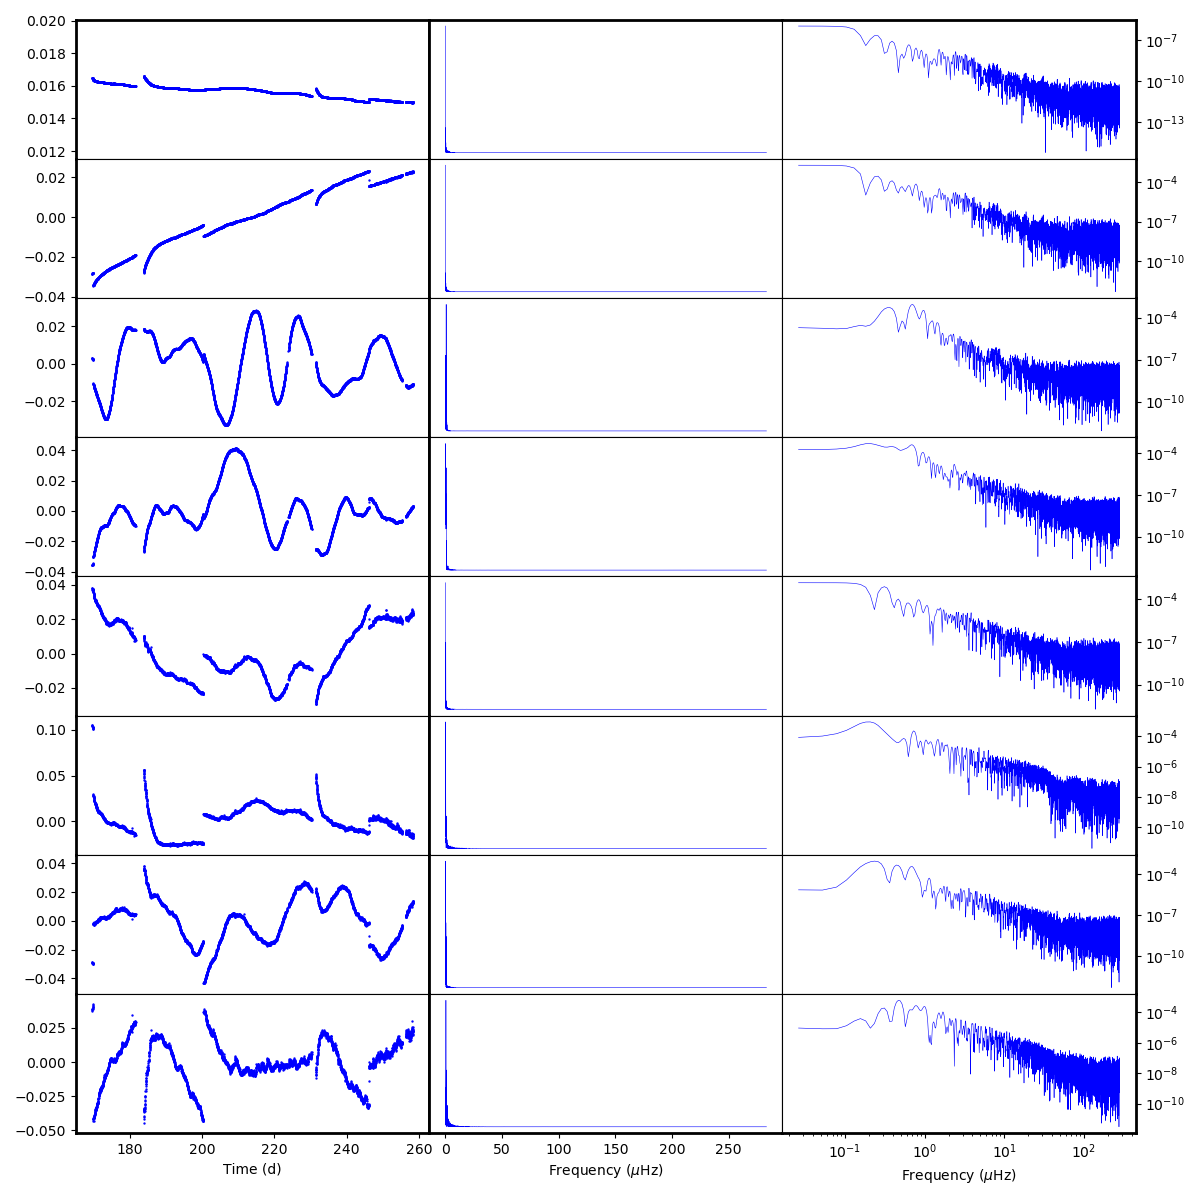
\includegraphics[width=0.9\linewidth]{Chapter_Appended/AppB/cbv_6791_q02.png}
    \caption{The first 8 co-trending basis vectors (CBVs) for NGC\,6791 for the second data quarter (left), and the Fourier transform of these vectors (middle), and in log-log space (right) from the full set of image subtracted light curves.}
    \label{fig:cbvs_allIS_6791_Q2}
\end{figure}


\begin{figure}
    \centering
    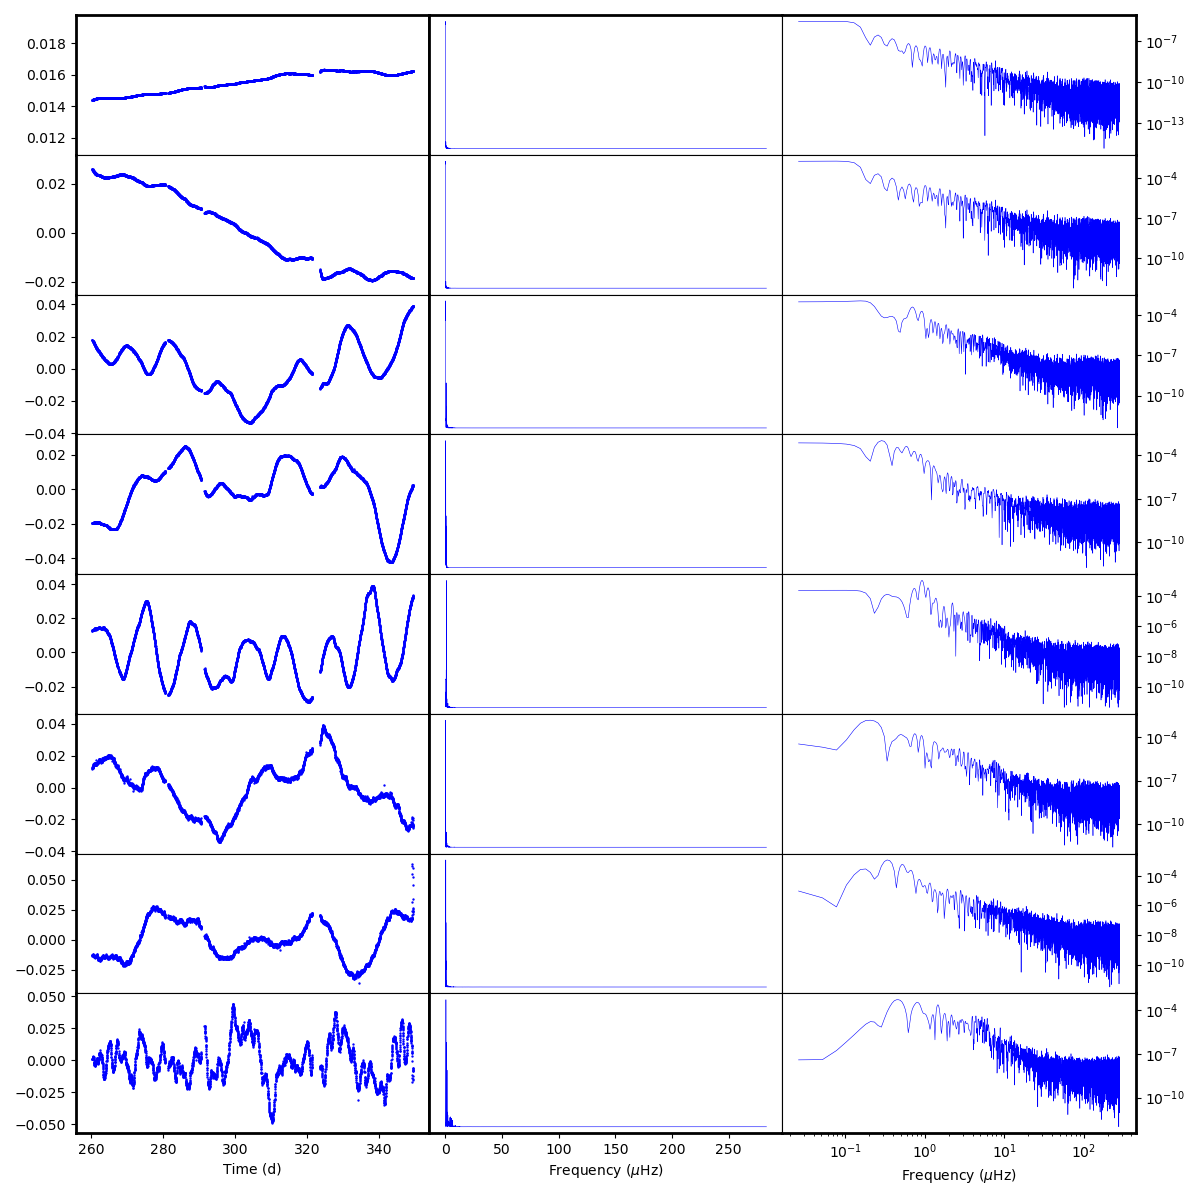
\includegraphics[width=\linewidth]{Chapter_Appended/AppB/cbv_6791_q03.png}
    \caption{Same as Figure \ref{fig:cbvs_allIS_6791_Q2} but for quarter 3.}
    \label{fig:cbvs_allIS_6791_Q03}
\end{figure}


\begin{figure}
    \centering
    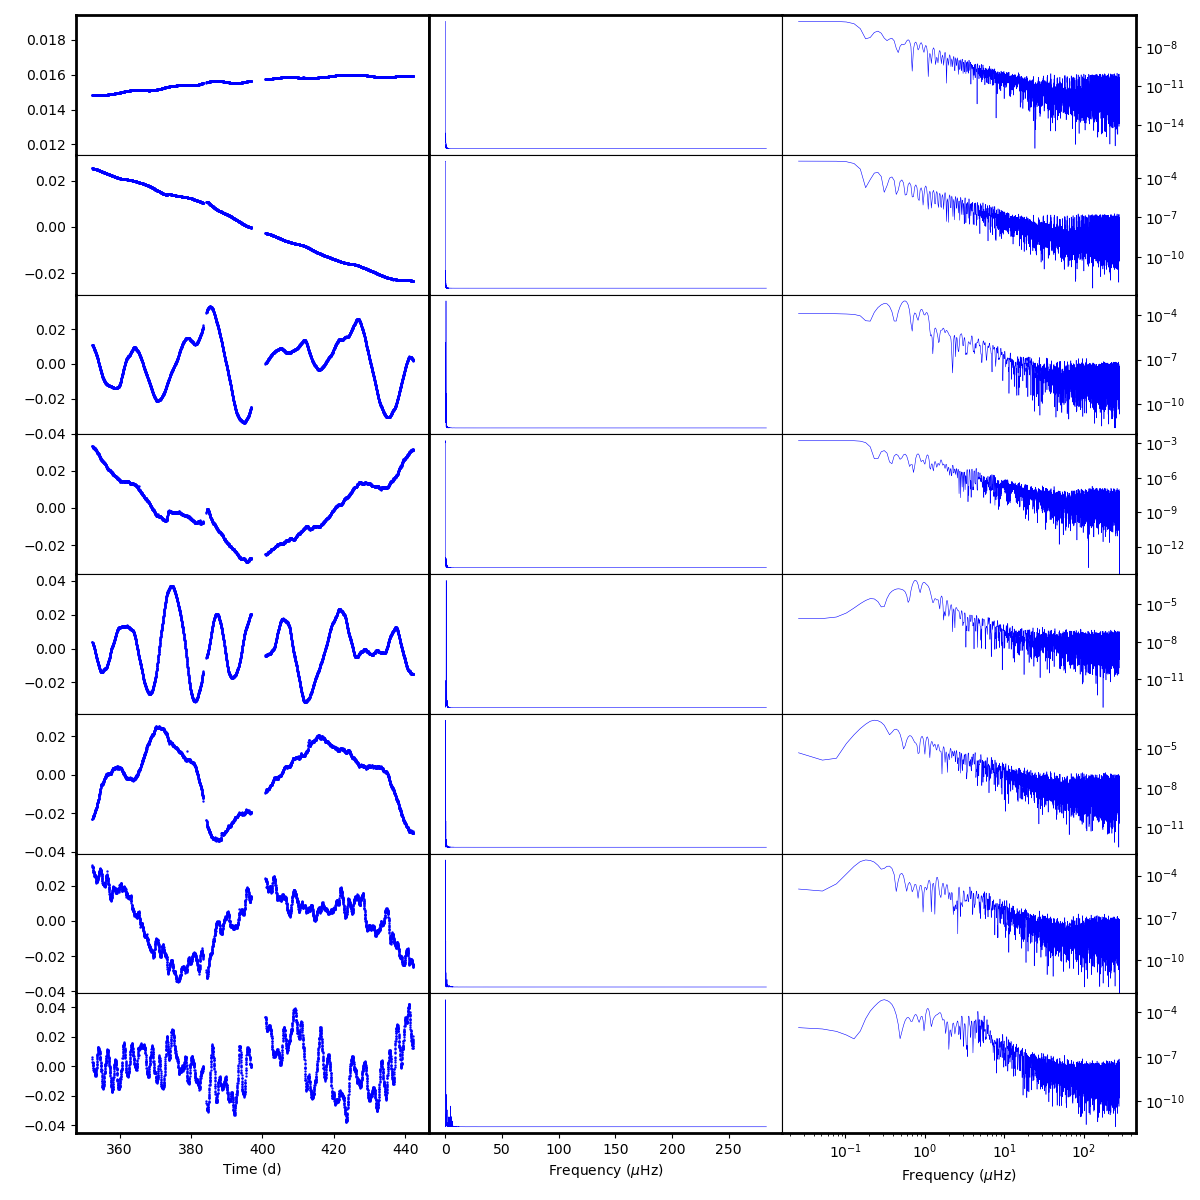
\includegraphics[width=\linewidth]{Chapter_Appended/AppB/cbv_6791_q04.png}
    \caption{Same as Figure \ref{fig:cbvs_allIS_6791_Q2} but for quarter 4.}
    \label{fig:cbvs_allIS_6791_Q04}
\end{figure}


\begin{figure}
    \centering
    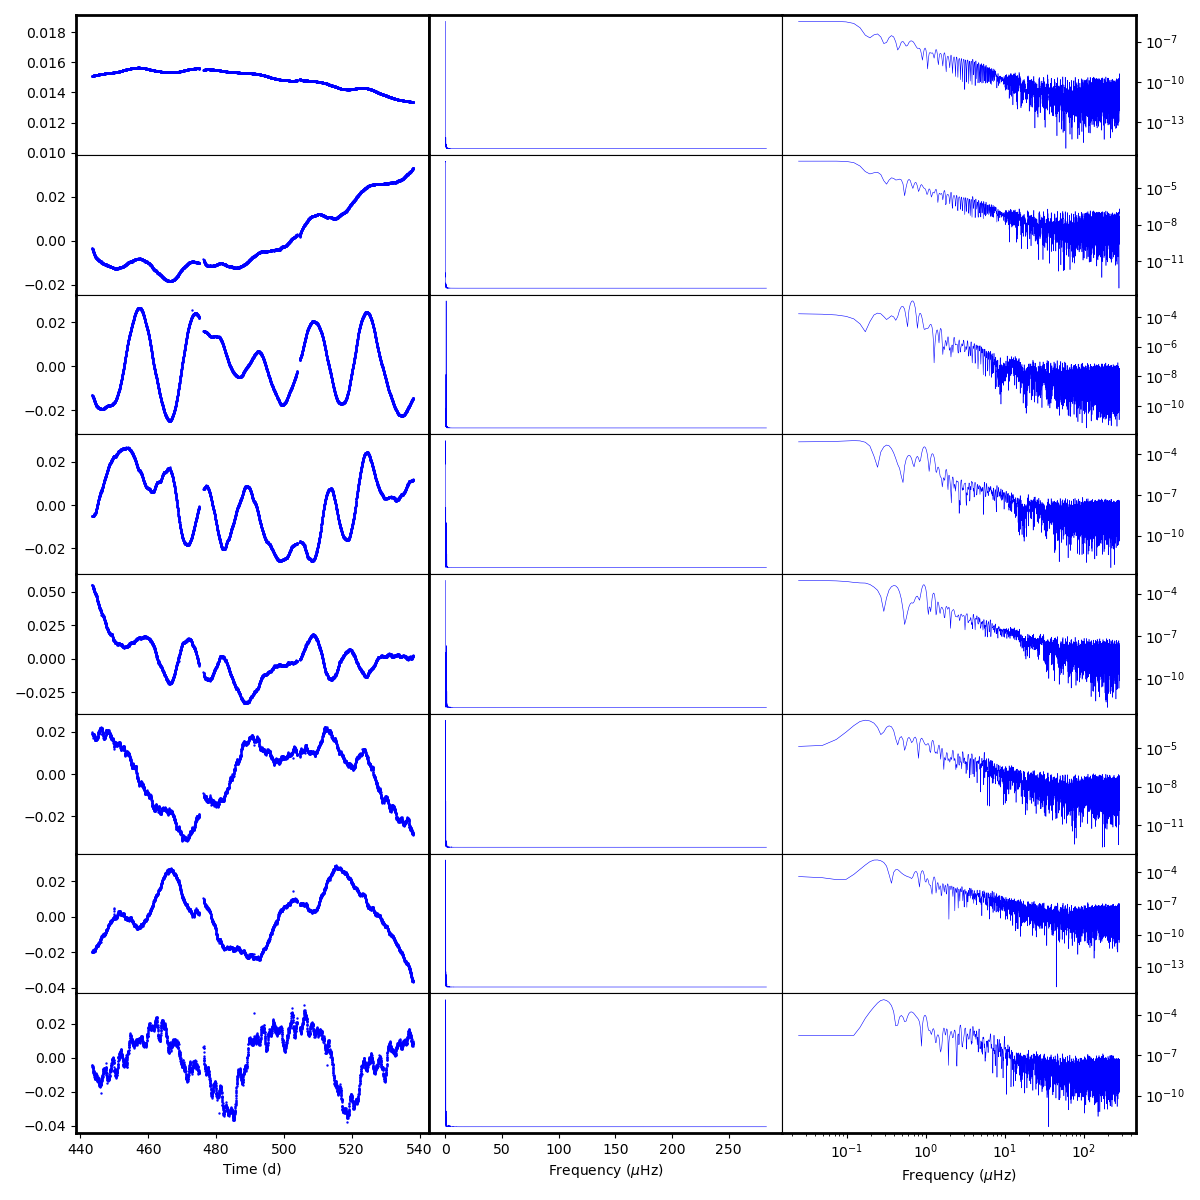
\includegraphics[width=\linewidth]{Chapter_Appended/AppB/cbv_6791_q05.png}
    \caption{Same as Figure \ref{fig:cbvs_allIS_6791_Q2} but for quarter 5.}
    \label{fig:cbvs_allIS_6791_Q05}
\end{figure}


\begin{figure}
    \centering
    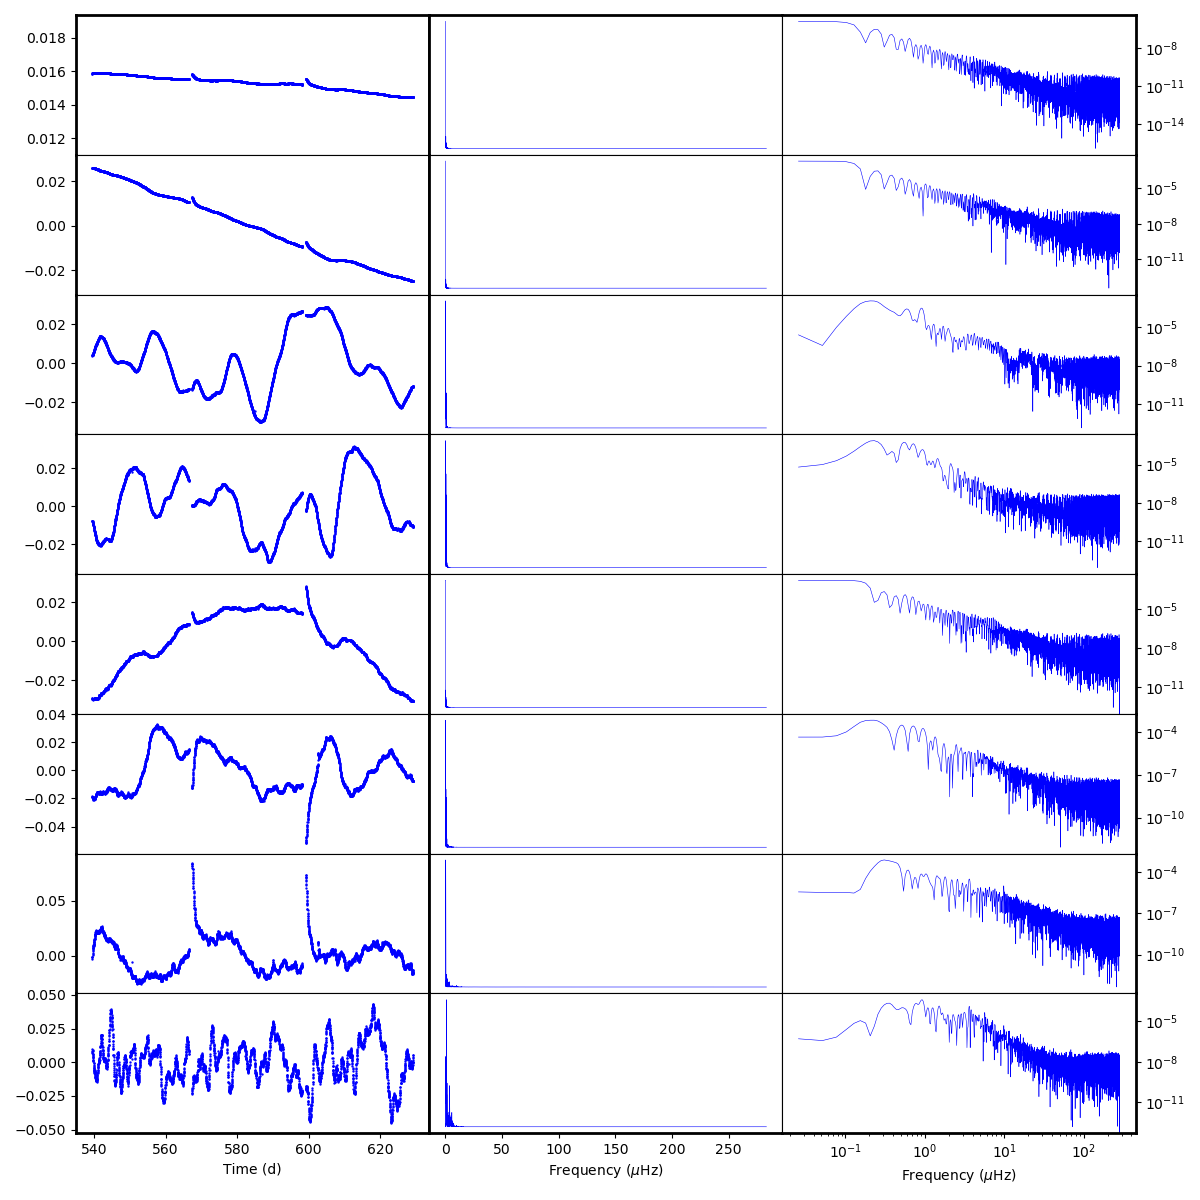
\includegraphics[width=\linewidth]{Chapter_Appended/AppB/cbv_6791_q06.png}
    \caption{Same as Figure \ref{fig:cbvs_allIS_6791_Q2} but for quarter 6.}
    \label{fig:cbvs_allIS_6791_Q06}
\end{figure}


\begin{figure}
    \centering
    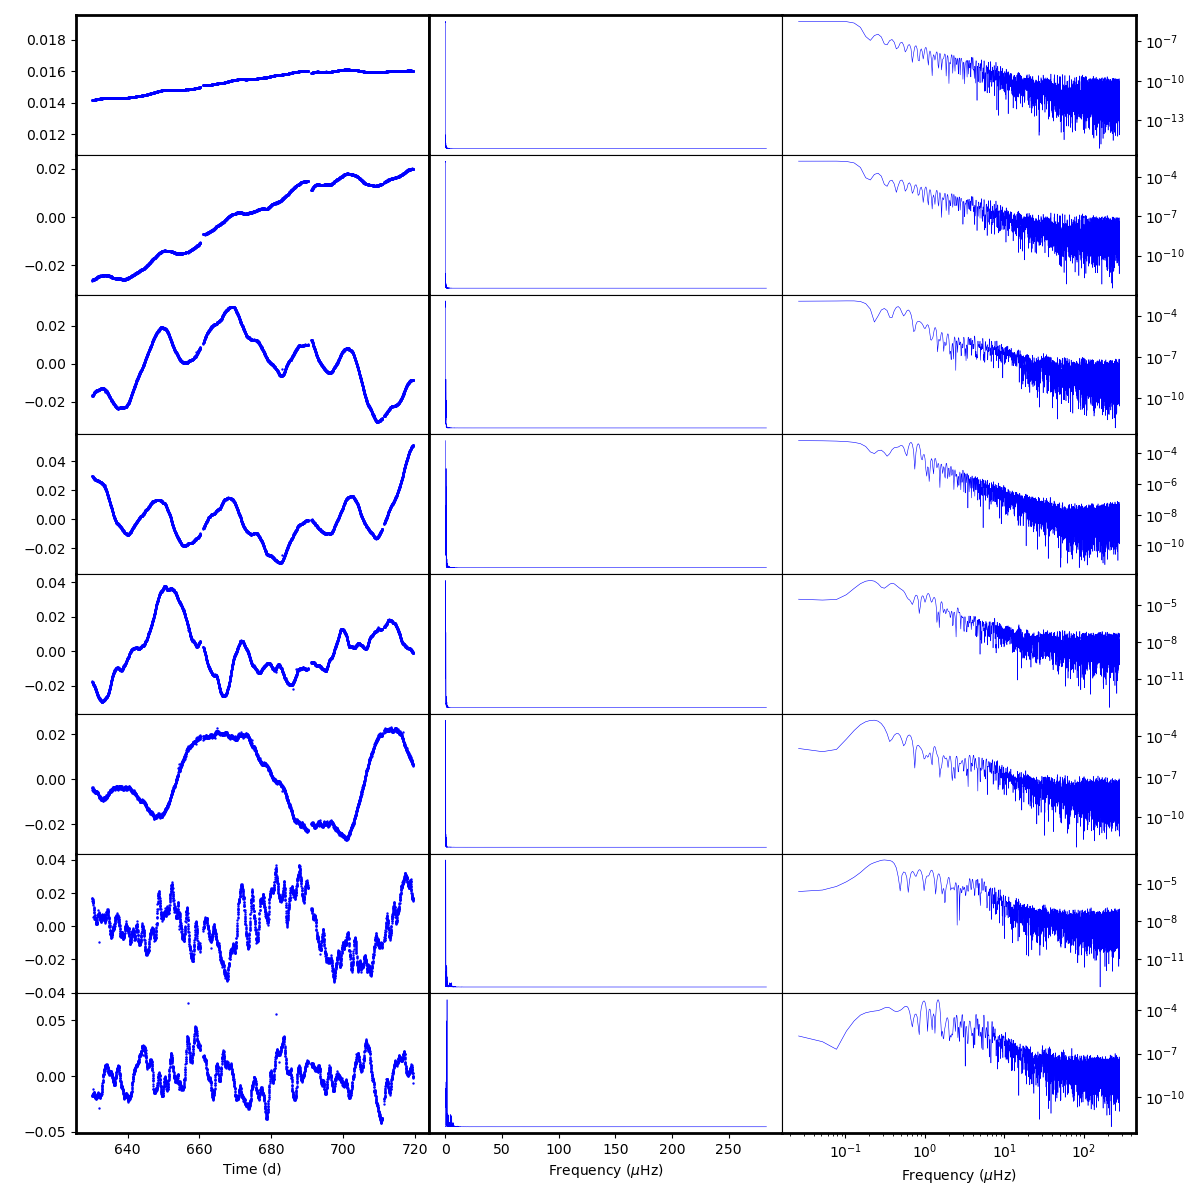
\includegraphics[width=\linewidth]{Chapter_Appended/AppB/cbv_6791_q07.png}
    \caption{Same as Figure \ref{fig:cbvs_allIS_6791_Q2} but for quarter 7.}
    \label{fig:cbvs_allIS_6791_Q07}
\end{figure}


\begin{figure}
    \centering
    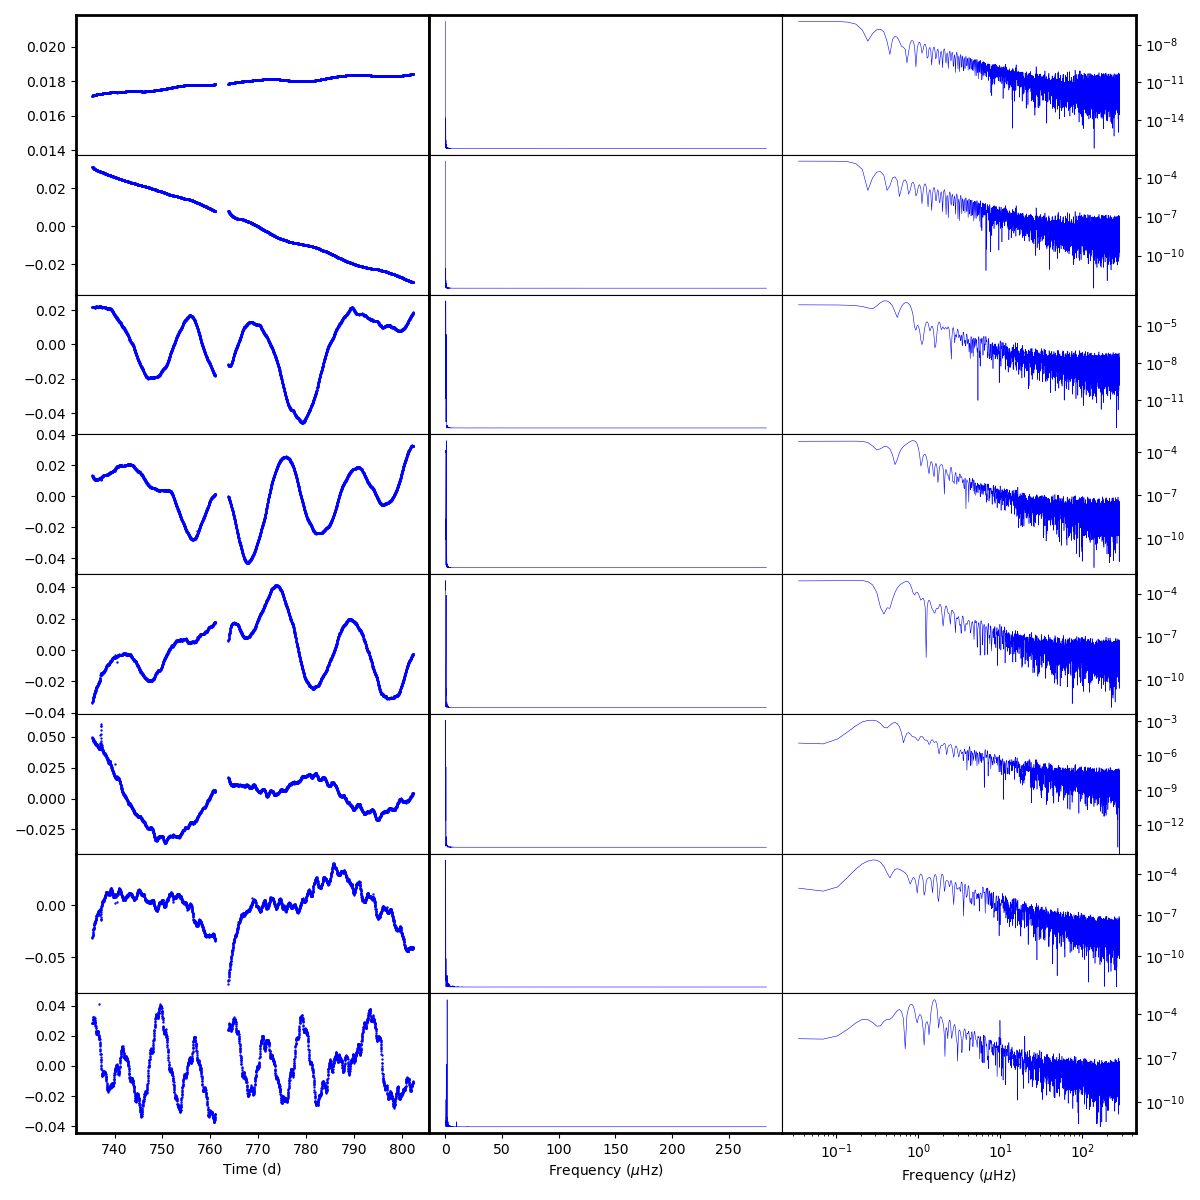
\includegraphics[width=\linewidth]{Chapter_Appended/AppB/cbv_6791_q08.png}
    \caption{Same as Figure \ref{fig:cbvs_allIS_6791_Q2} but for quarter 8.}
    \label{fig:cbvs_allIS_6791_Q08}
\end{figure}


\begin{figure}
    \centering
    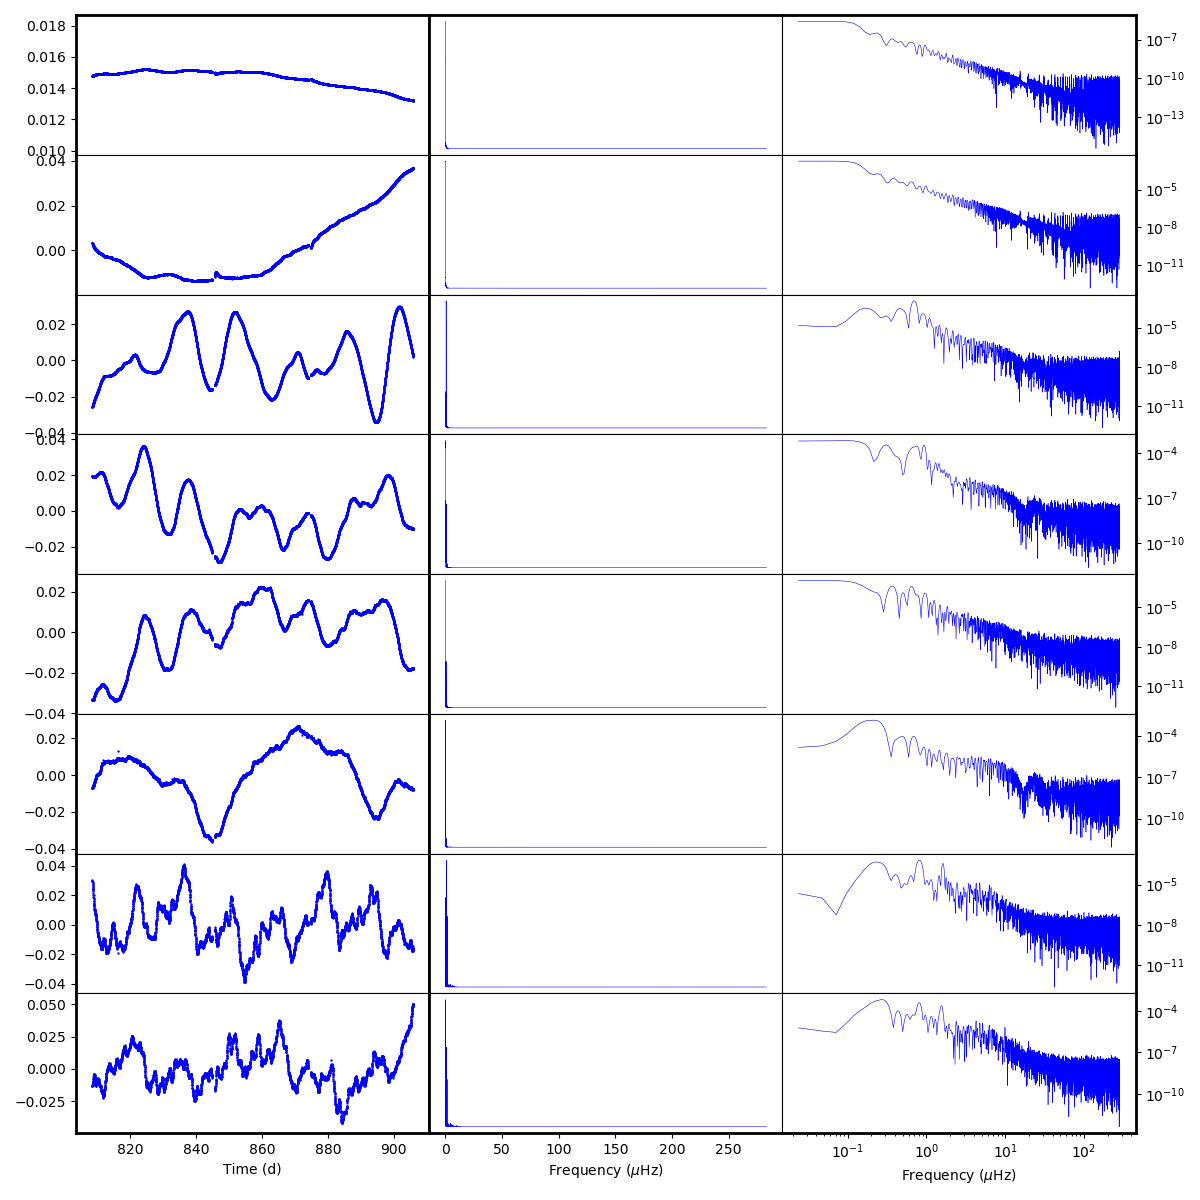
\includegraphics[width=\linewidth]{Chapter_Appended/AppB/cbv_6791_q09.png}
    \caption{Same as Figure \ref{fig:cbvs_allIS_6791_Q2} but for quarter 9.}
    \label{fig:cbvs_allIS_6791_Q09}
\end{figure}


\begin{figure}
    \centering
    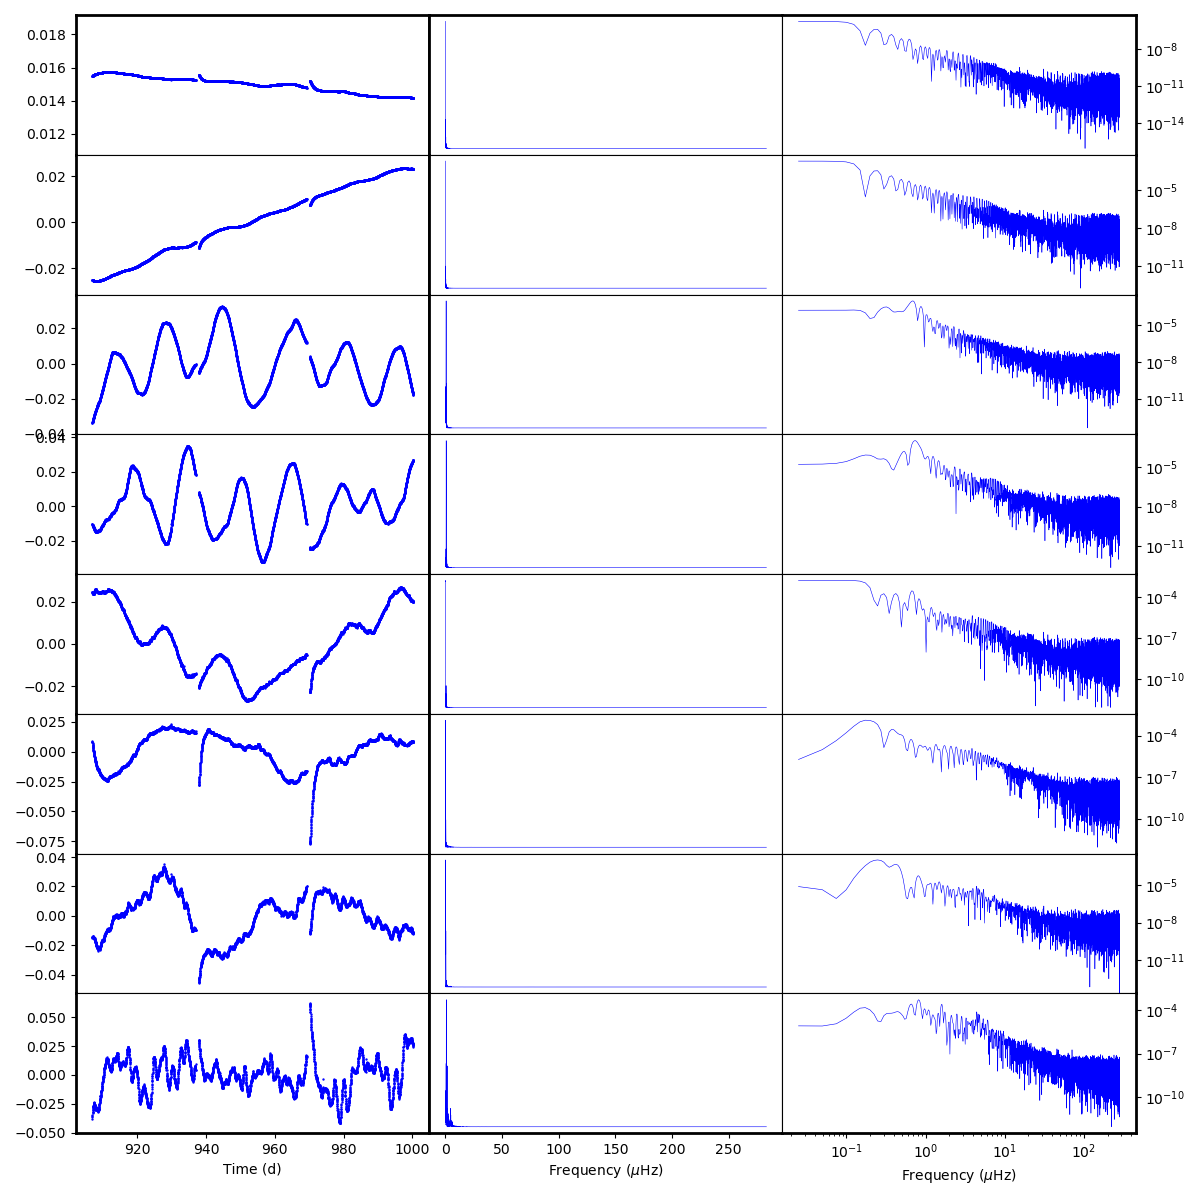
\includegraphics[width=\linewidth]{Chapter_Appended/AppB/cbv_6791_q10.png}
    \caption{Same as Figure \ref{fig:cbvs_allIS_6791_Q2} but for quarter 10.}
    \label{fig:cbvs_allIS_6791_Q10}
\end{figure}


\begin{figure}
    \centering
    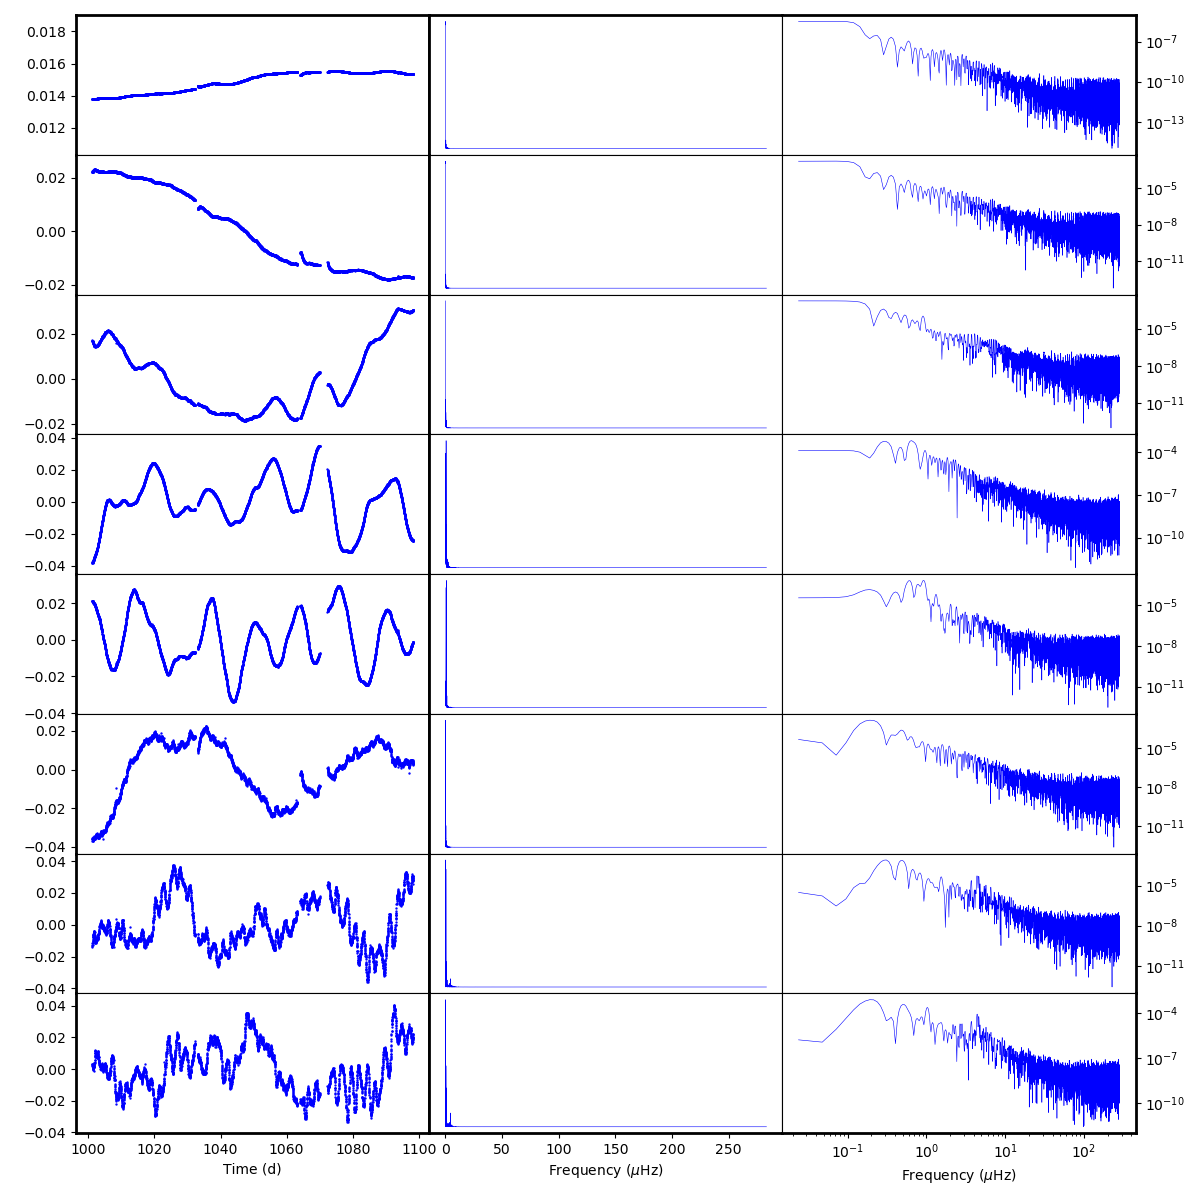
\includegraphics[width=\linewidth]{Chapter_Appended/AppB/cbv_6791_q11.png}
    \caption{Same as Figure \ref{fig:cbvs_allIS_6791_Q2} but for quarter 11.}
    \label{fig:cbvs_allIS_6791_Q11}
\end{figure}


\begin{figure}
    \centering
    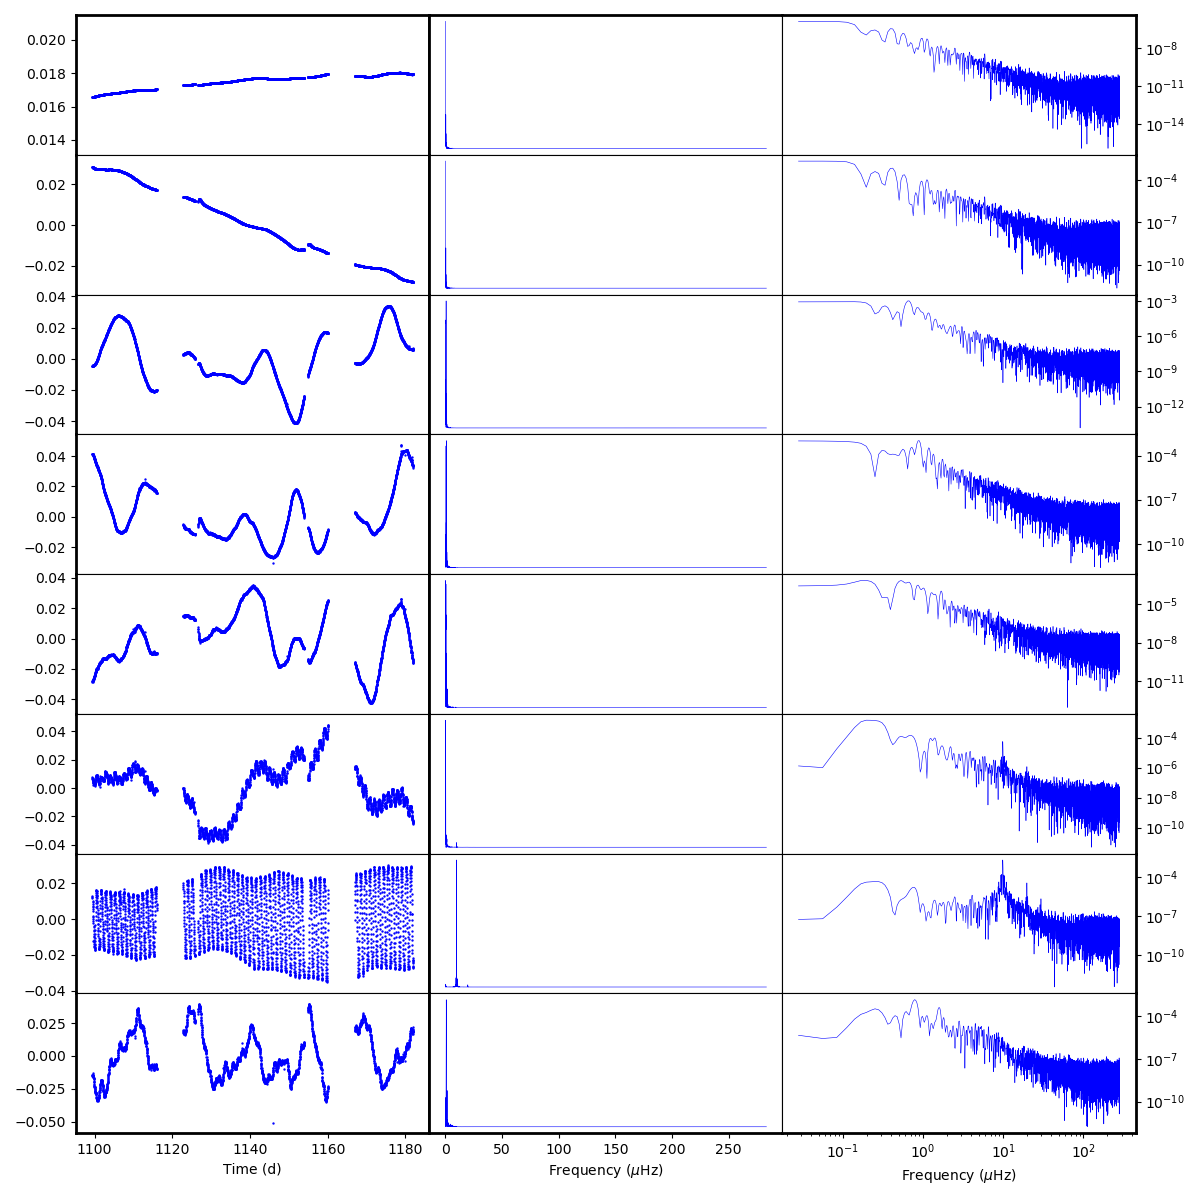
\includegraphics[width=\linewidth]{Chapter_Appended/AppB/cbv_6791_q12.png}
    \caption{Same as Figure \ref{fig:cbvs_allIS_6791_Q2} but for quarter 12.}
    \label{fig:cbvs_allIS_6791_Q12}
\end{figure}


\begin{figure}
    \centering
    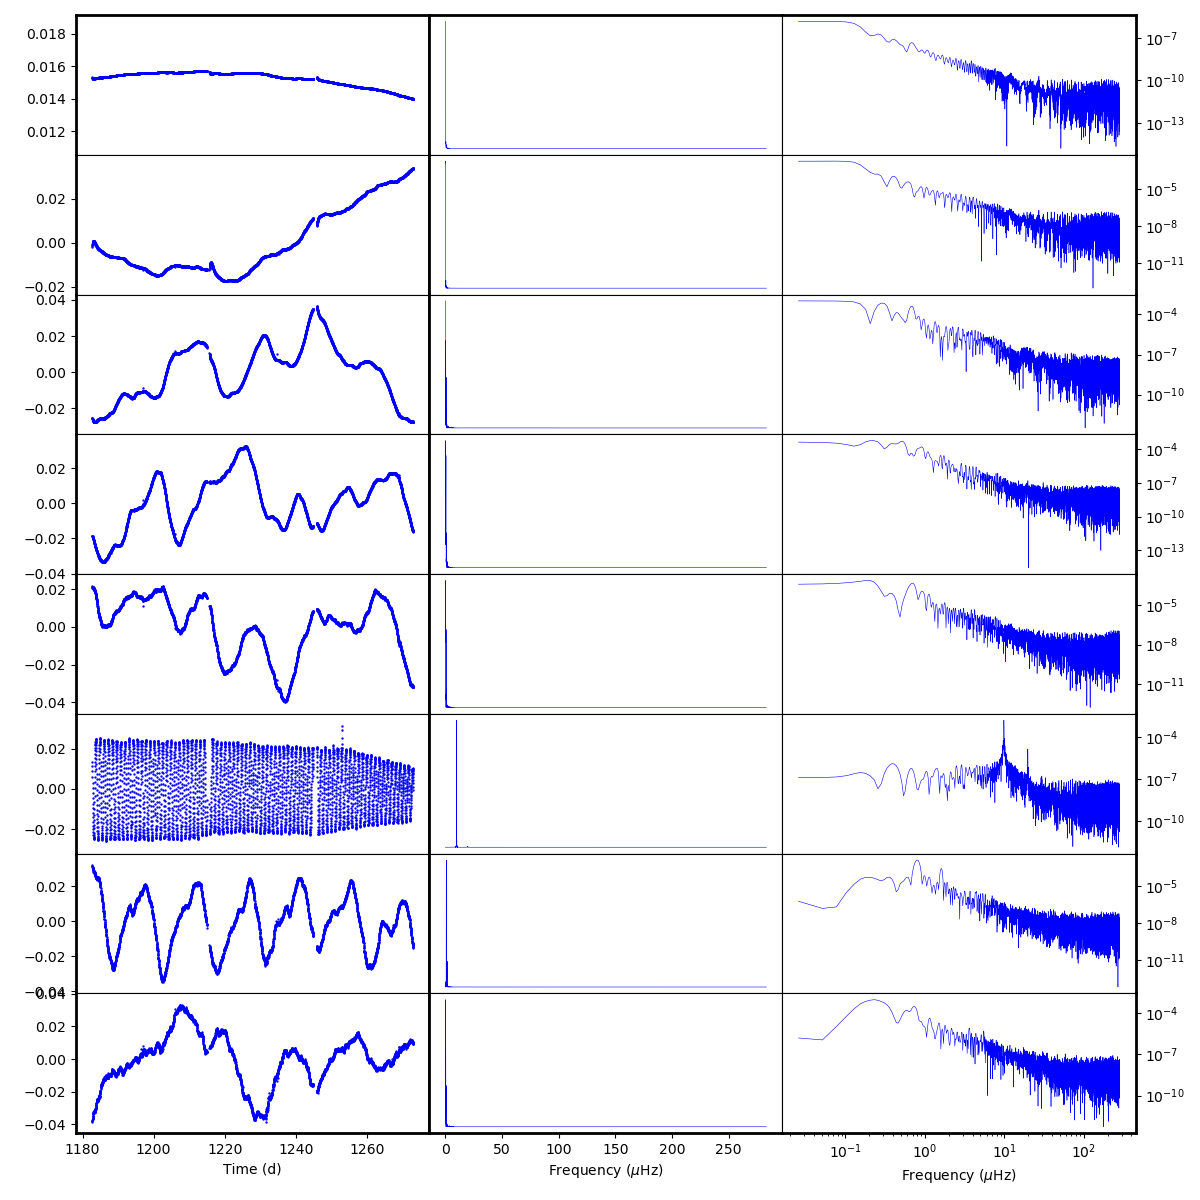
\includegraphics[width=\linewidth]{Chapter_Appended/AppB/cbv_6791_q13.png}
    \caption{Same as Figure \ref{fig:cbvs_allIS_6791_Q2} but for quarter 13.}
    \label{fig:cbvs_allIS_6791_Q13}
\end{figure}


\begin{figure}
    \centering
    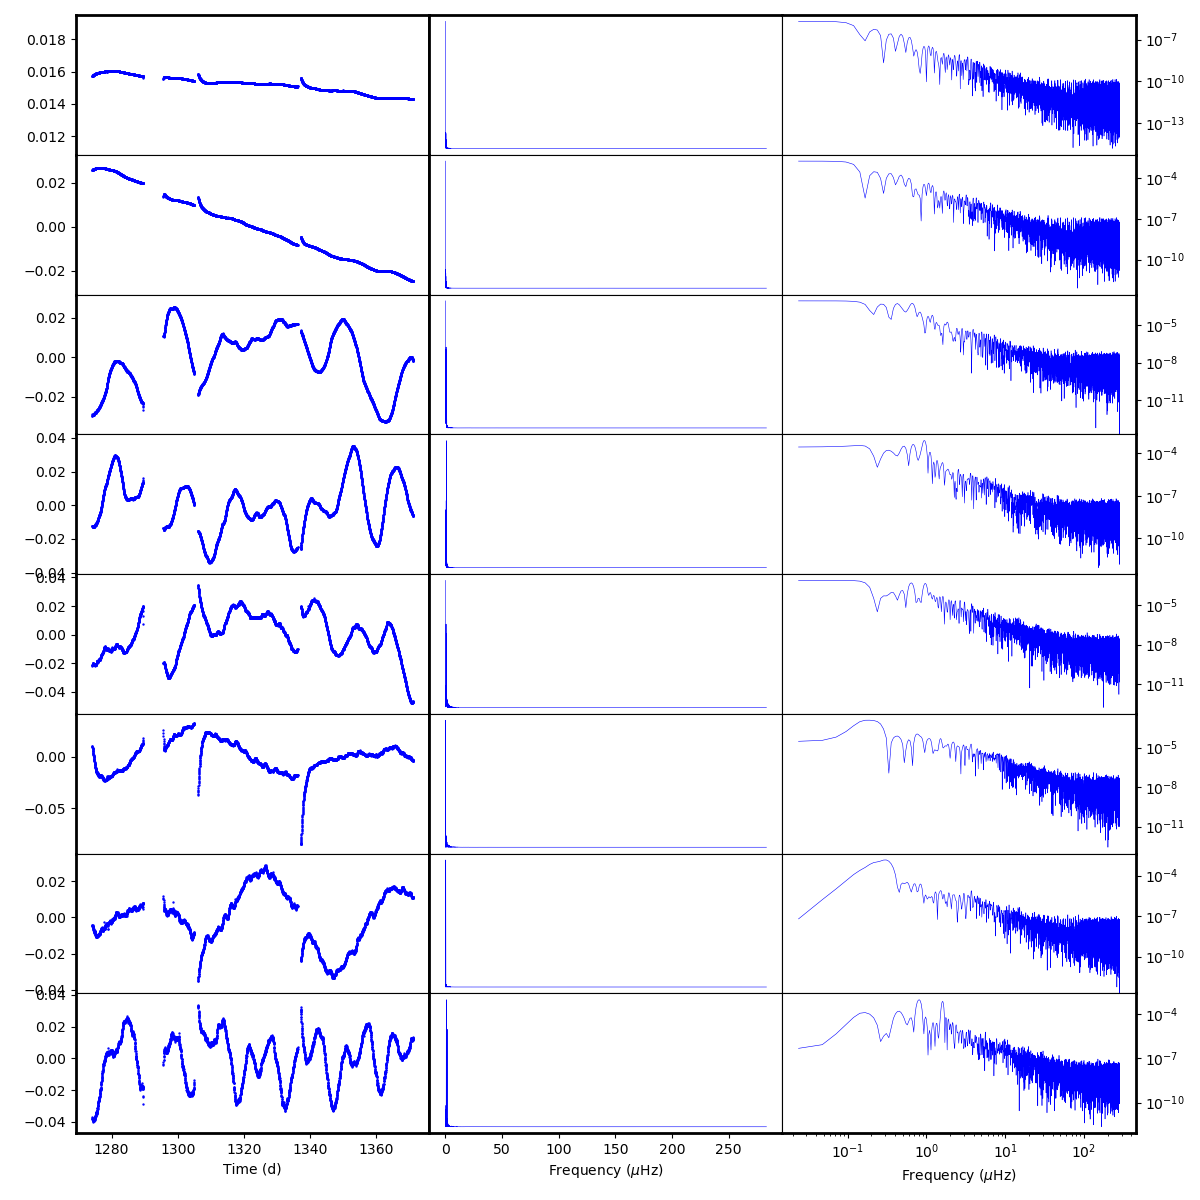
\includegraphics[width=\linewidth]{Chapter_Appended/AppB/cbv_6791_q14.png}
    \caption{Same as Figure \ref{fig:cbvs_allIS_6791_Q2} but for quarter 14.}
    \label{fig:cbvs_allIS_6791_Q14}
\end{figure}


\begin{figure}
    \centering
    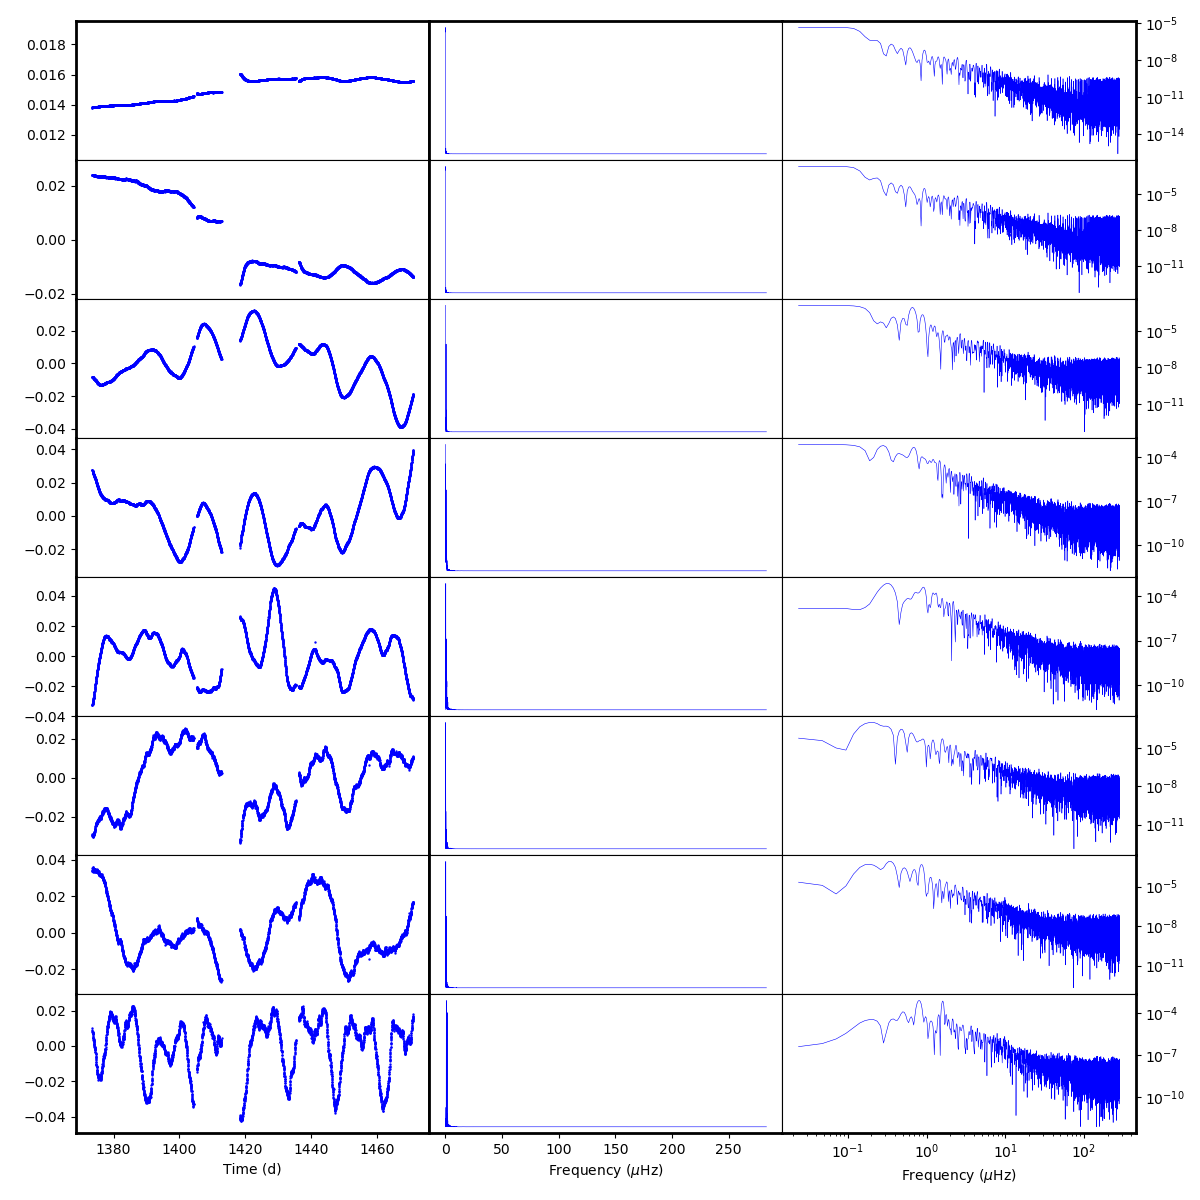
\includegraphics[width=\linewidth]{Chapter_Appended/AppB/cbv_6791_q15.png}
    \caption{Same as Figure \ref{fig:cbvs_allIS_6791_Q2} but for quarter 15.}
    \label{fig:cbvs_allIS_6791_Q15}
\end{figure}


\begin{figure}
    \centering
    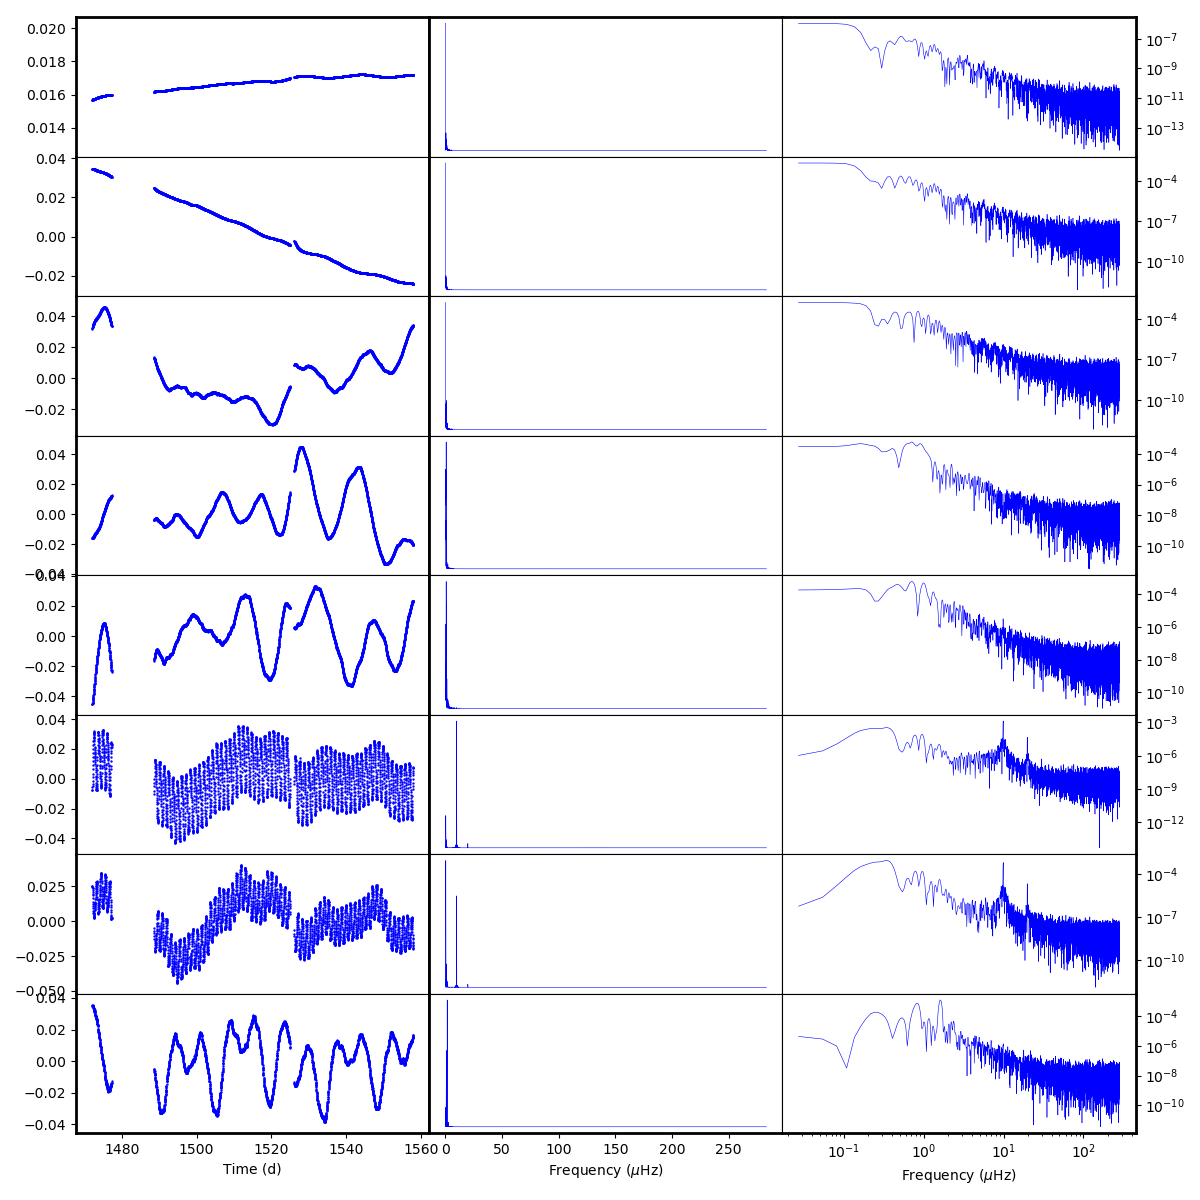
\includegraphics[width=\linewidth]{Chapter_Appended/AppB/cbv_6791_q16.png}
    \caption{Same as Figure \ref{fig:cbvs_allIS_6791_Q2} but for quarter 16.}
    \label{fig:cbvs_allIS_6791_Q16}
\end{figure}


\begin{figure}
    \centering
    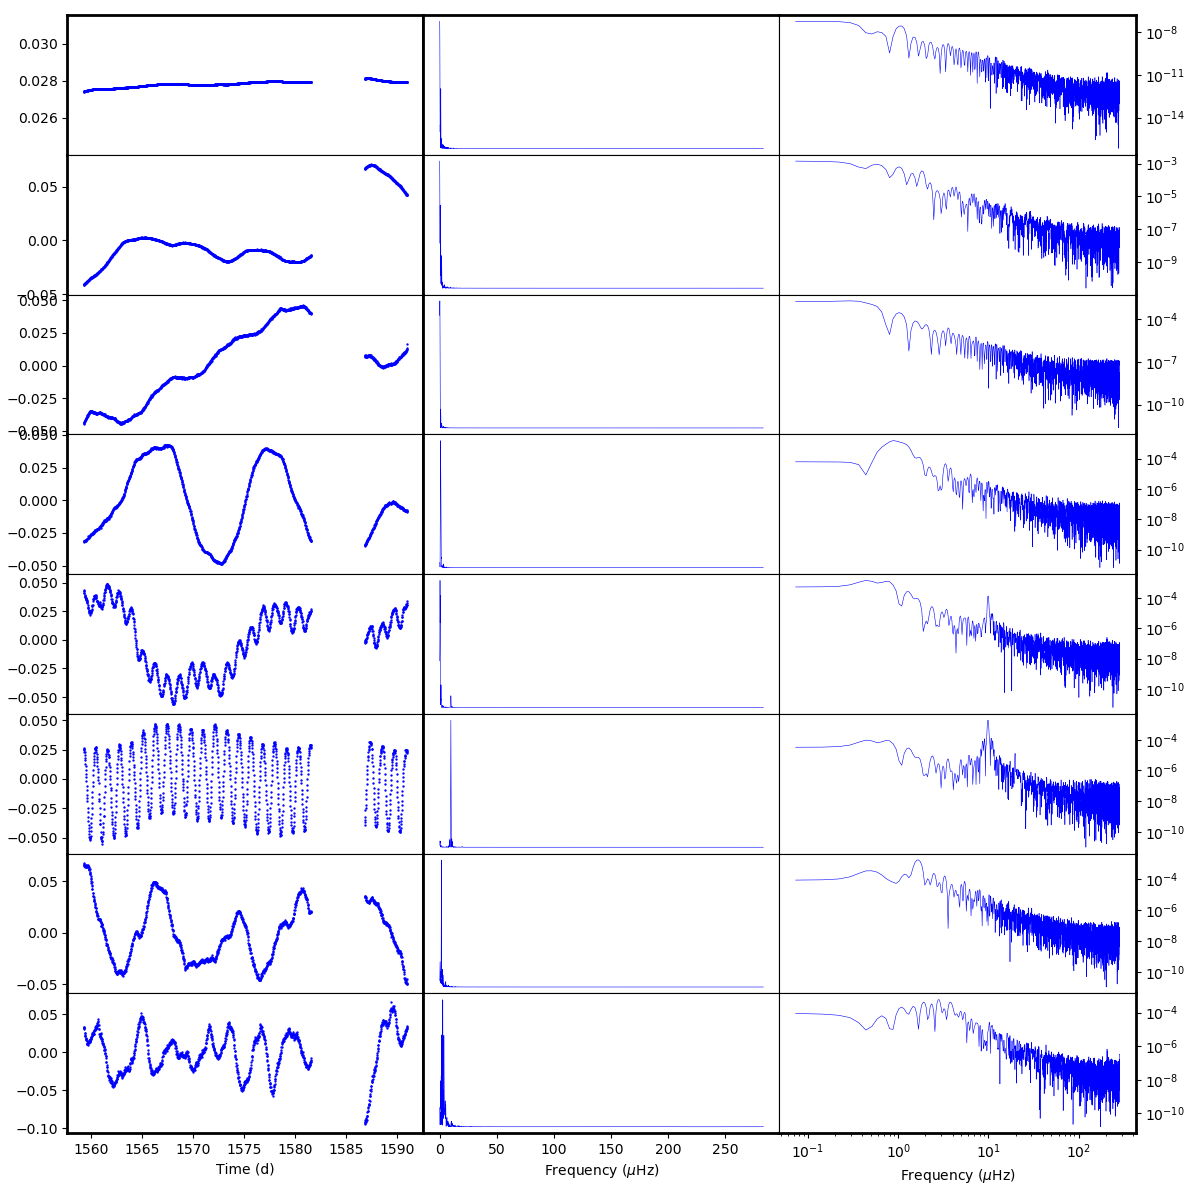
\includegraphics[width=\linewidth]{Chapter_Appended/AppB/cbv_6791_q17.png}
    \caption{Same as Figure \ref{fig:cbvs_allIS_6791_Q2} but for quarter 17.}
    \label{fig:cbvs_allIS_6791_Q17}
\end{figure}


\begin{figure}
    \centering
    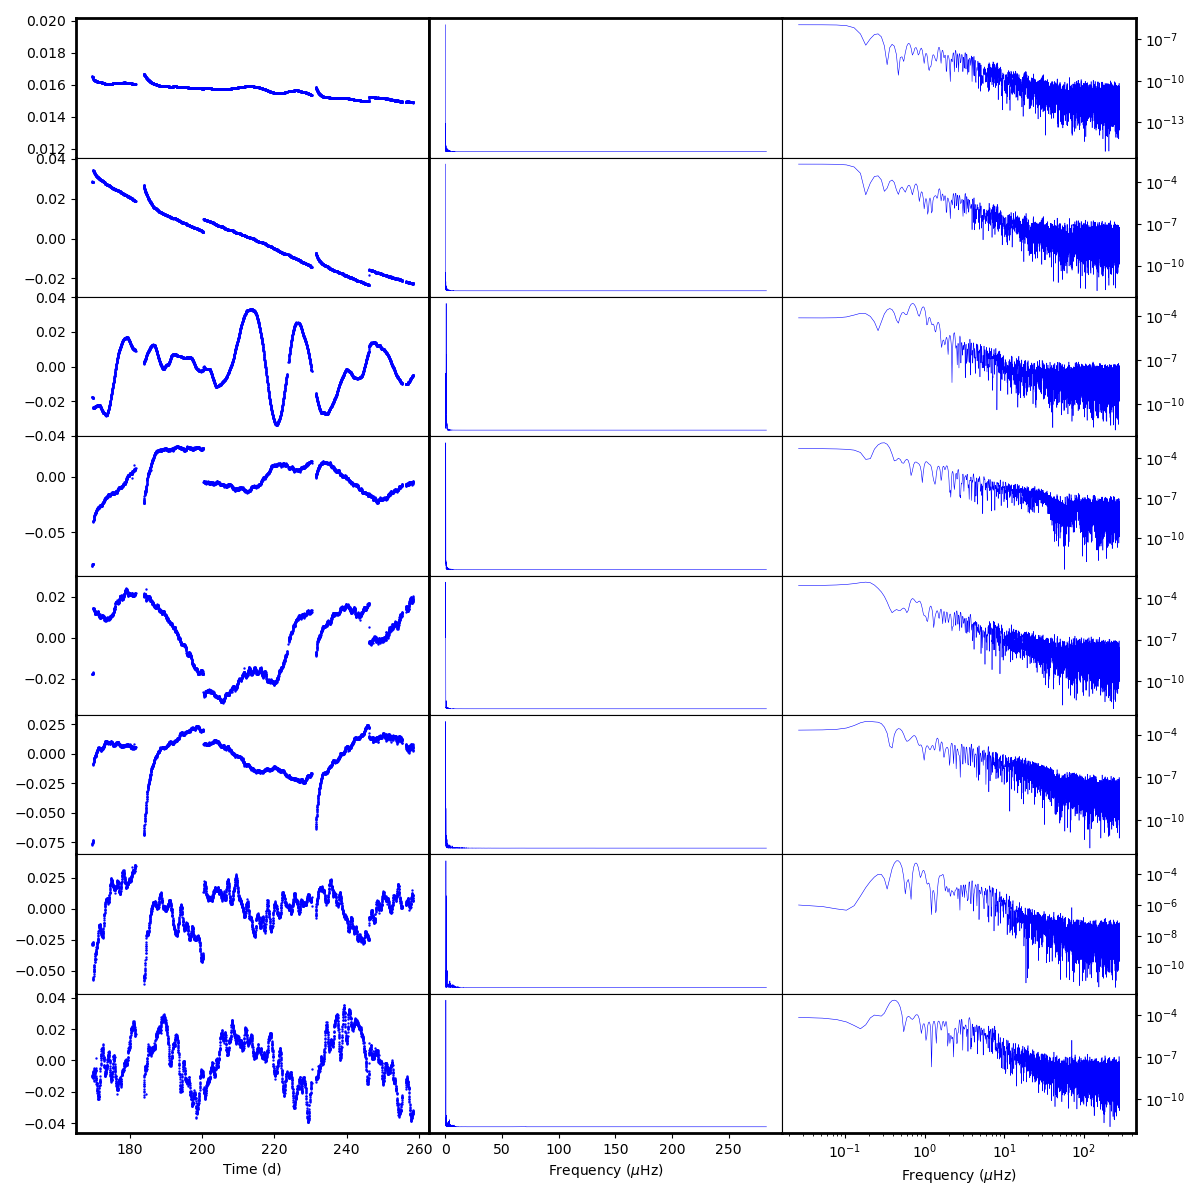
\includegraphics[width=\linewidth]{Chapter_Appended/AppB/cbv_6791_rgs_q02.png}
    \caption{The first 8 co-trending basis vectors (CBVs) for NGC\,6791 for the second data quarter (left), and the Fourier transform of these vectors (middle), and in log-log space (right) from the likely red giant member subset of image subtracted light curves.}
    \label{fig:cbvs_rgsIS_6791_Q2}
\end{figure}


\begin{figure}
    \centering
    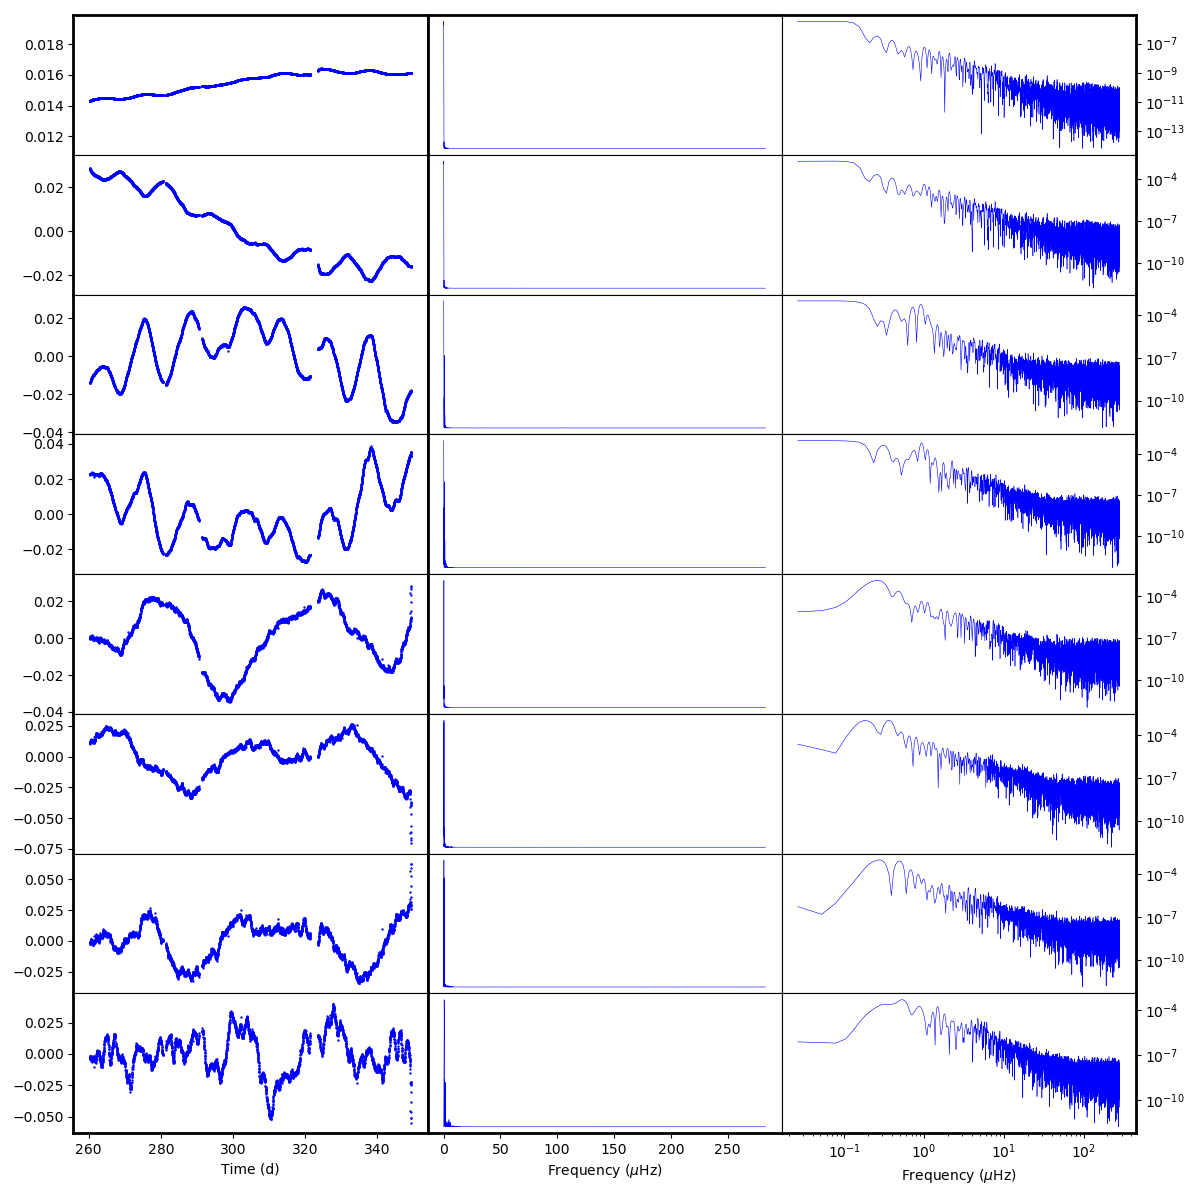
\includegraphics[width=\linewidth]{Chapter_Appended/AppB/cbv_6791_rgs_q03.png}
    \caption{Same as Figure \ref{fig:cbvs_rgsIS_6791_Q2} but for quarter 3.}
    \label{fig:cbvs_rgsIS_6791_Q03}
\end{figure}


\begin{figure}
    \centering
    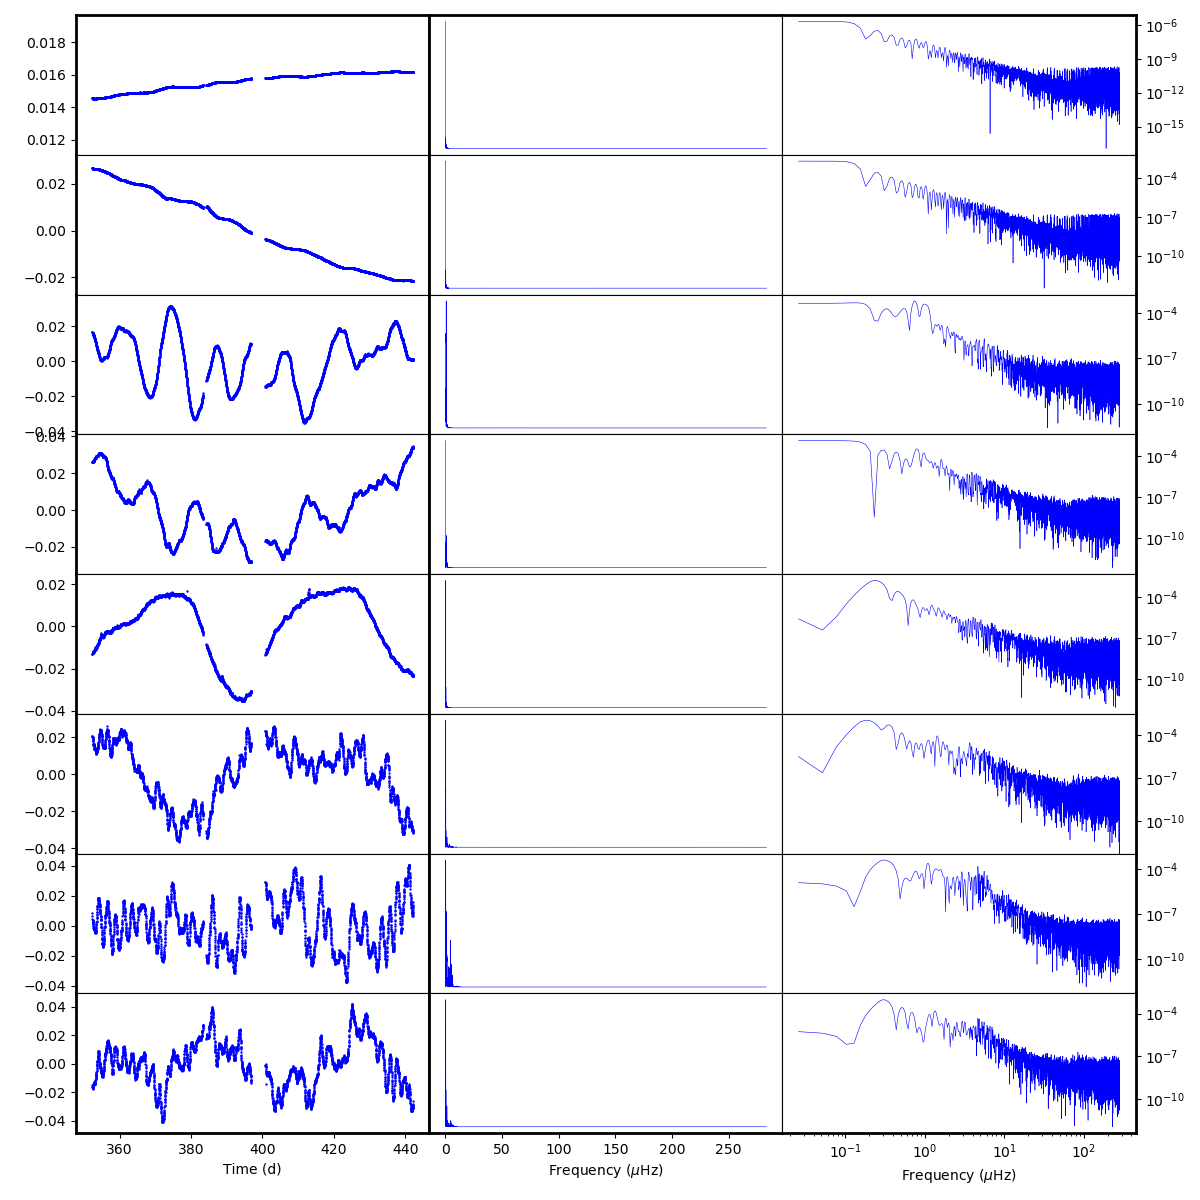
\includegraphics[width=\linewidth]{Chapter_Appended/AppB/cbv_6791_rgs_q04.png}
    \caption{Same as Figure \ref{fig:cbvs_rgsIS_6791_Q2} but for quarter 4.}
    \label{fig:cbvs_rgsIS_6791_Q04}
\end{figure}


\begin{figure}
    \centering
    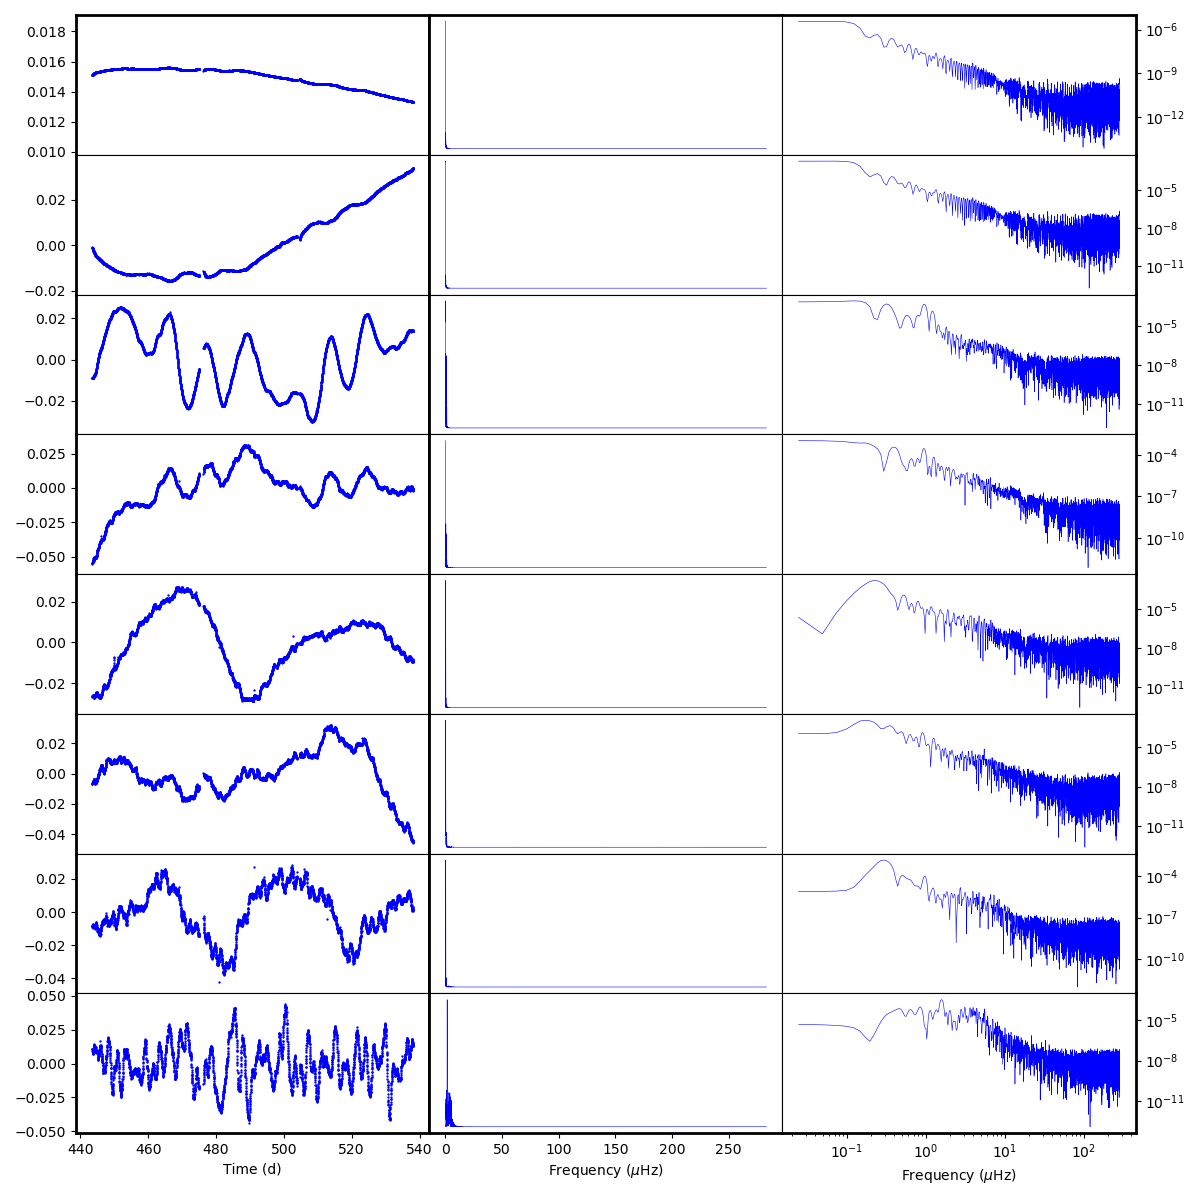
\includegraphics[width=\linewidth]{Chapter_Appended/AppB/cbv_6791_rgs_q05.png}
    \caption{Same as Figure \ref{fig:cbvs_rgsIS_6791_Q2} but for quarter 5.}
    \label{fig:cbvs_rgsIS_6791_Q05}
\end{figure}


\begin{figure}
    \centering
    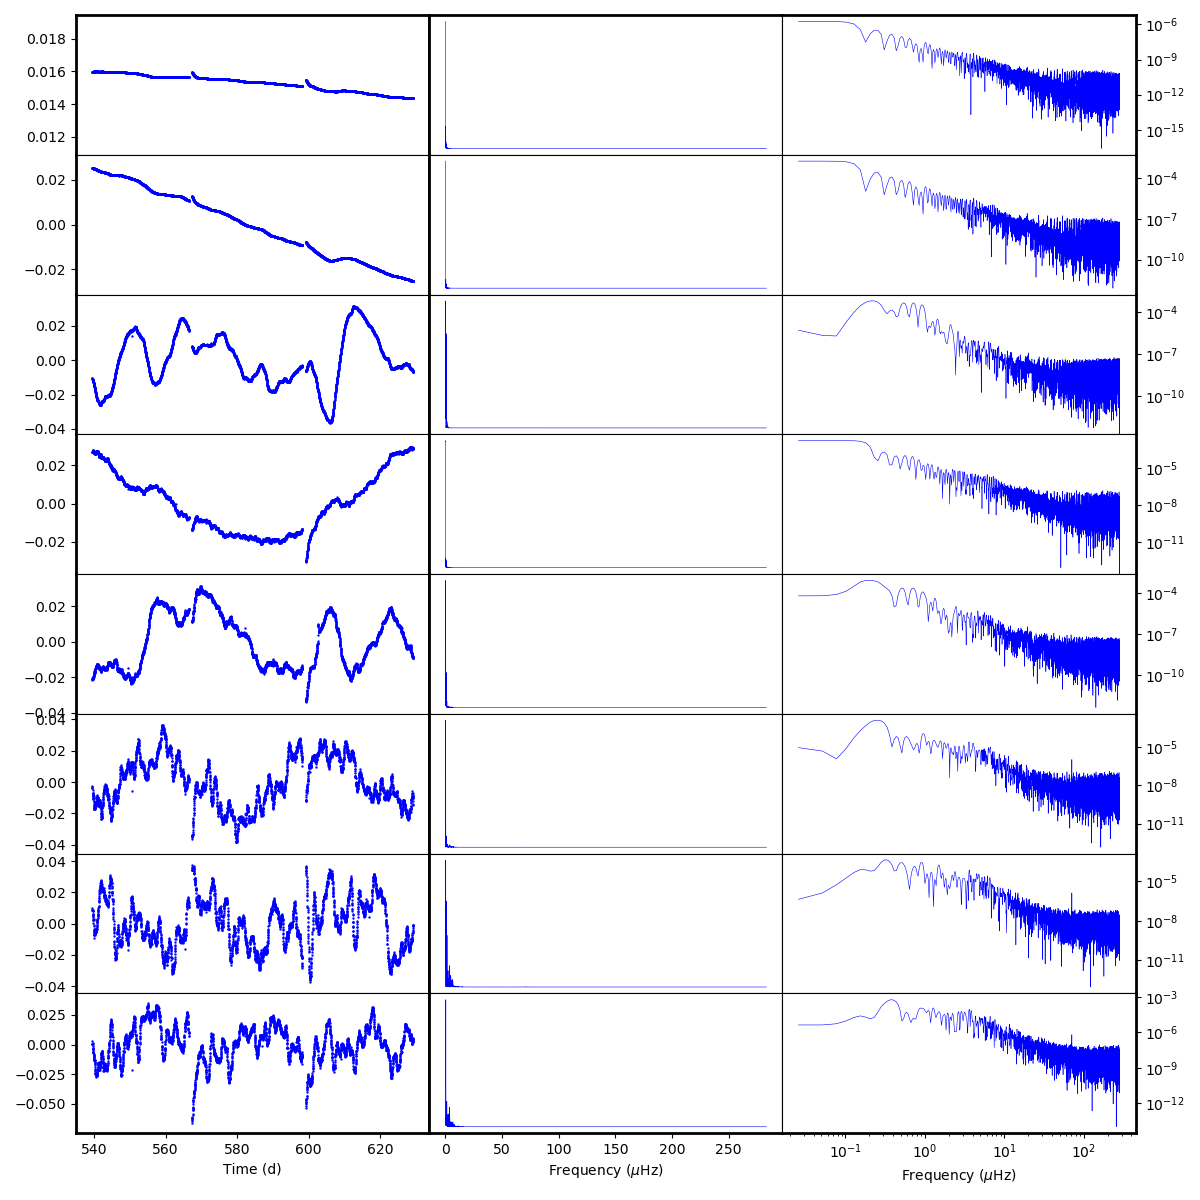
\includegraphics[width=\linewidth]{Chapter_Appended/AppB/cbv_6791_rgs_q06.png}
    \caption{Same as Figure \ref{fig:cbvs_rgsIS_6791_Q2} but for quarter 6.}
    \label{fig:cbvs_rgsIS_6791_Q06}
\end{figure}


\begin{figure}
    \centering
    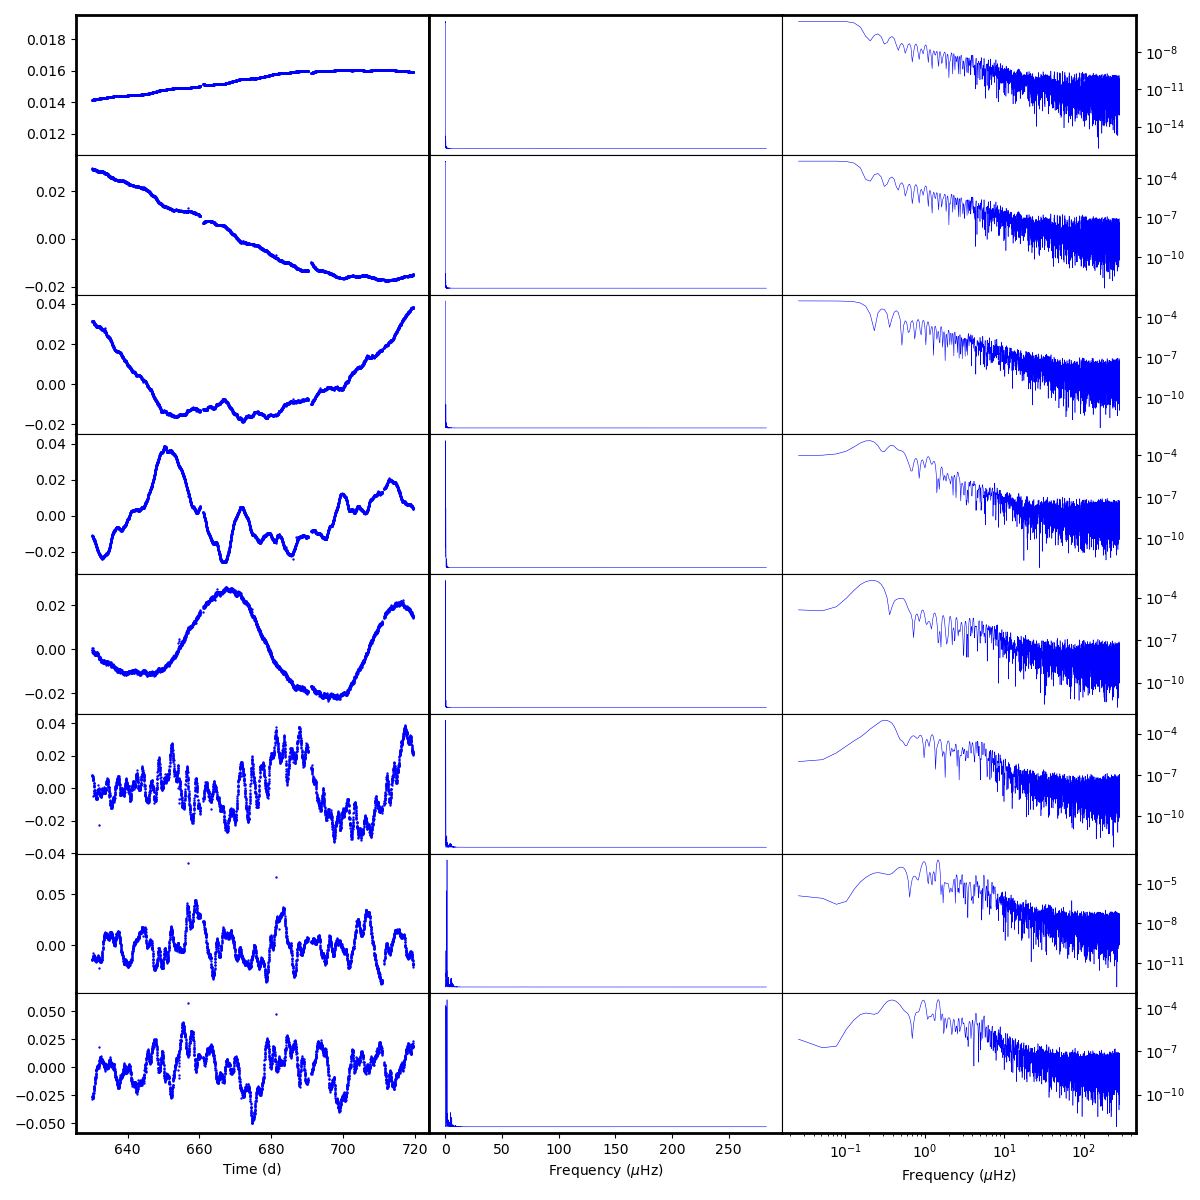
\includegraphics[width=\linewidth]{Chapter_Appended/AppB/cbv_6791_rgs_q07.png}
    \caption{Same as Figure \ref{fig:cbvs_rgsIS_6791_Q2} but for quarter 7.}
    \label{fig:cbvs_rgsIS_6791_Q07}
\end{figure}


\begin{figure}
    \centering
    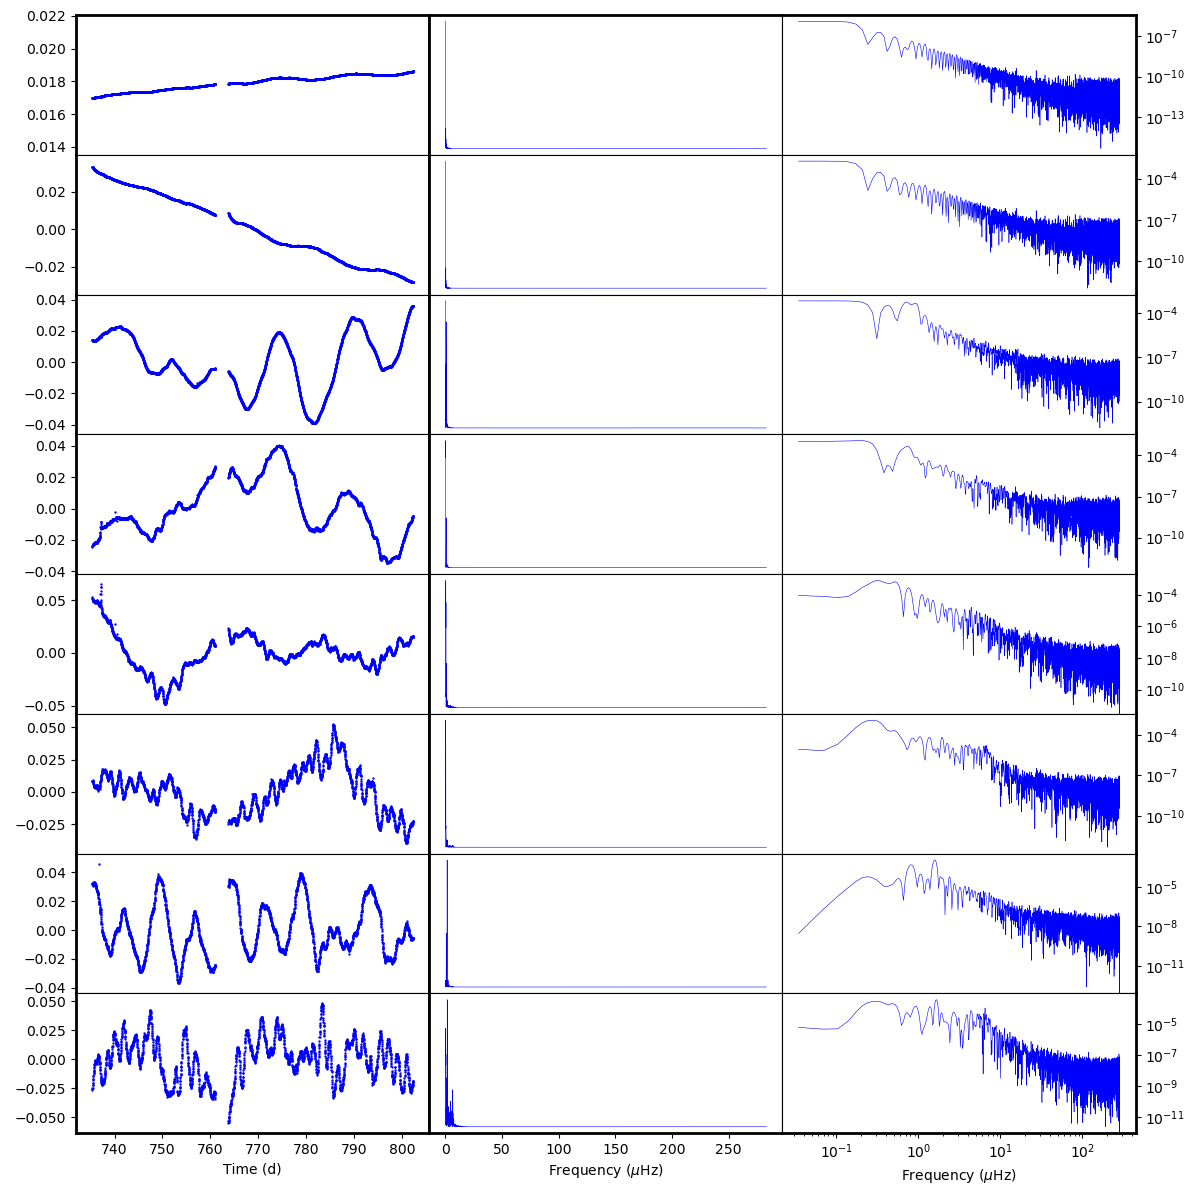
\includegraphics[width=\linewidth]{Chapter_Appended/AppB/cbv_6791_rgs_q08.png}
    \caption{Same as Figure \ref{fig:cbvs_rgsIS_6791_Q2} but for quarter 8.}
    \label{fig:cbvs_rgsIS_6791_Q08}
\end{figure}


\begin{figure}
    \centering
    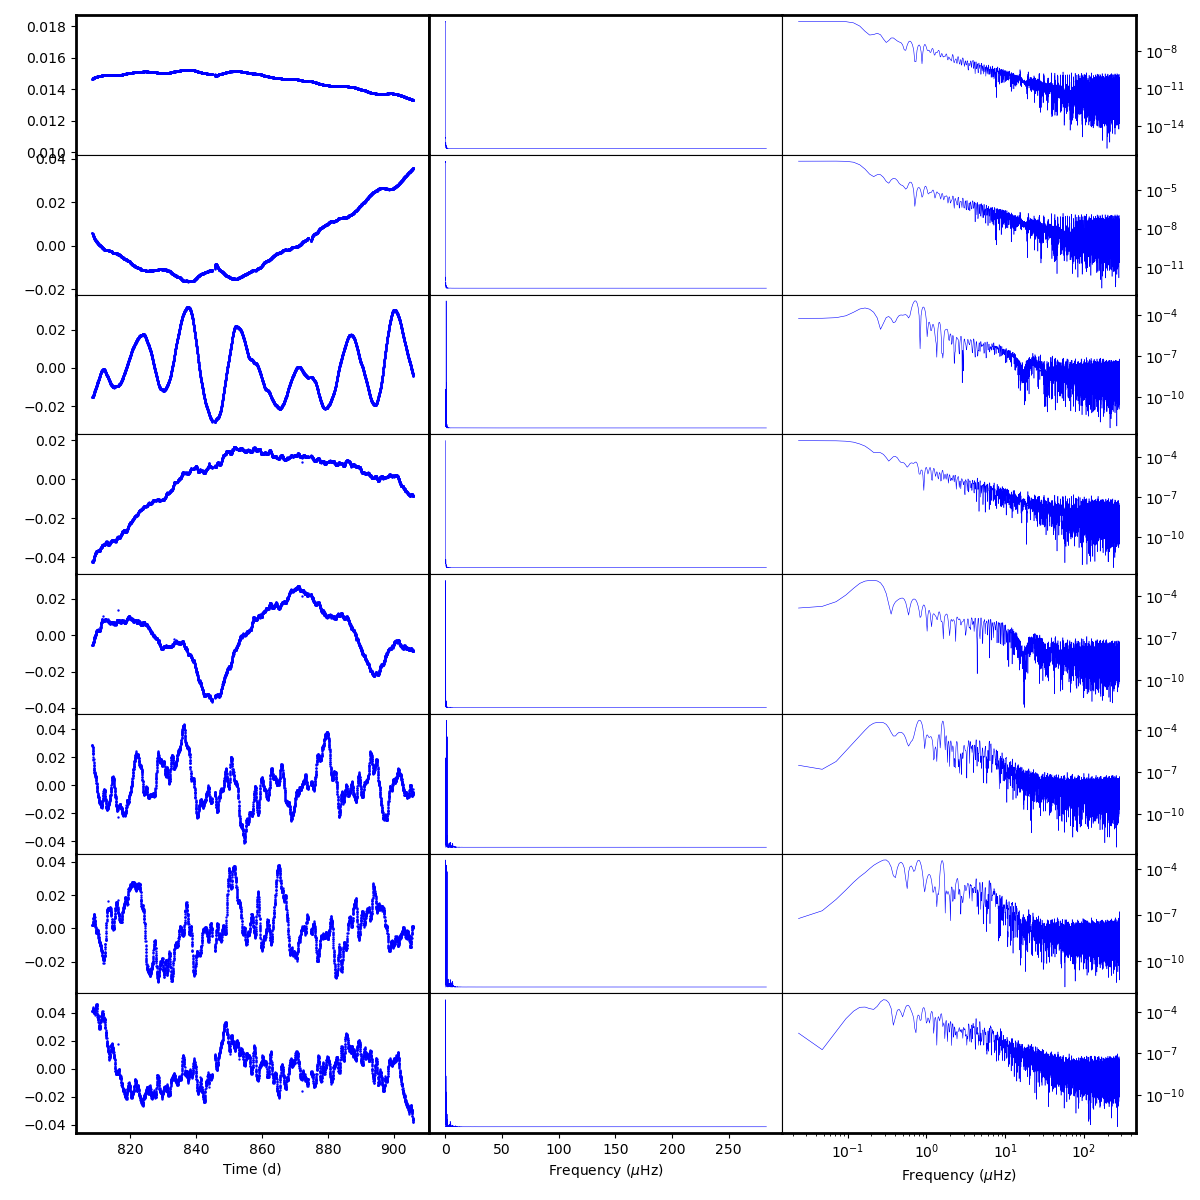
\includegraphics[width=\linewidth]{Chapter_Appended/AppB/cbv_6791_rgs_q09.png}
    \caption{Same as Figure \ref{fig:cbvs_rgsIS_6791_Q2} but for quarter 9.}
    \label{fig:cbvs_rgsIS_6791_Q09}
\end{figure}


\begin{figure}
    \centering
    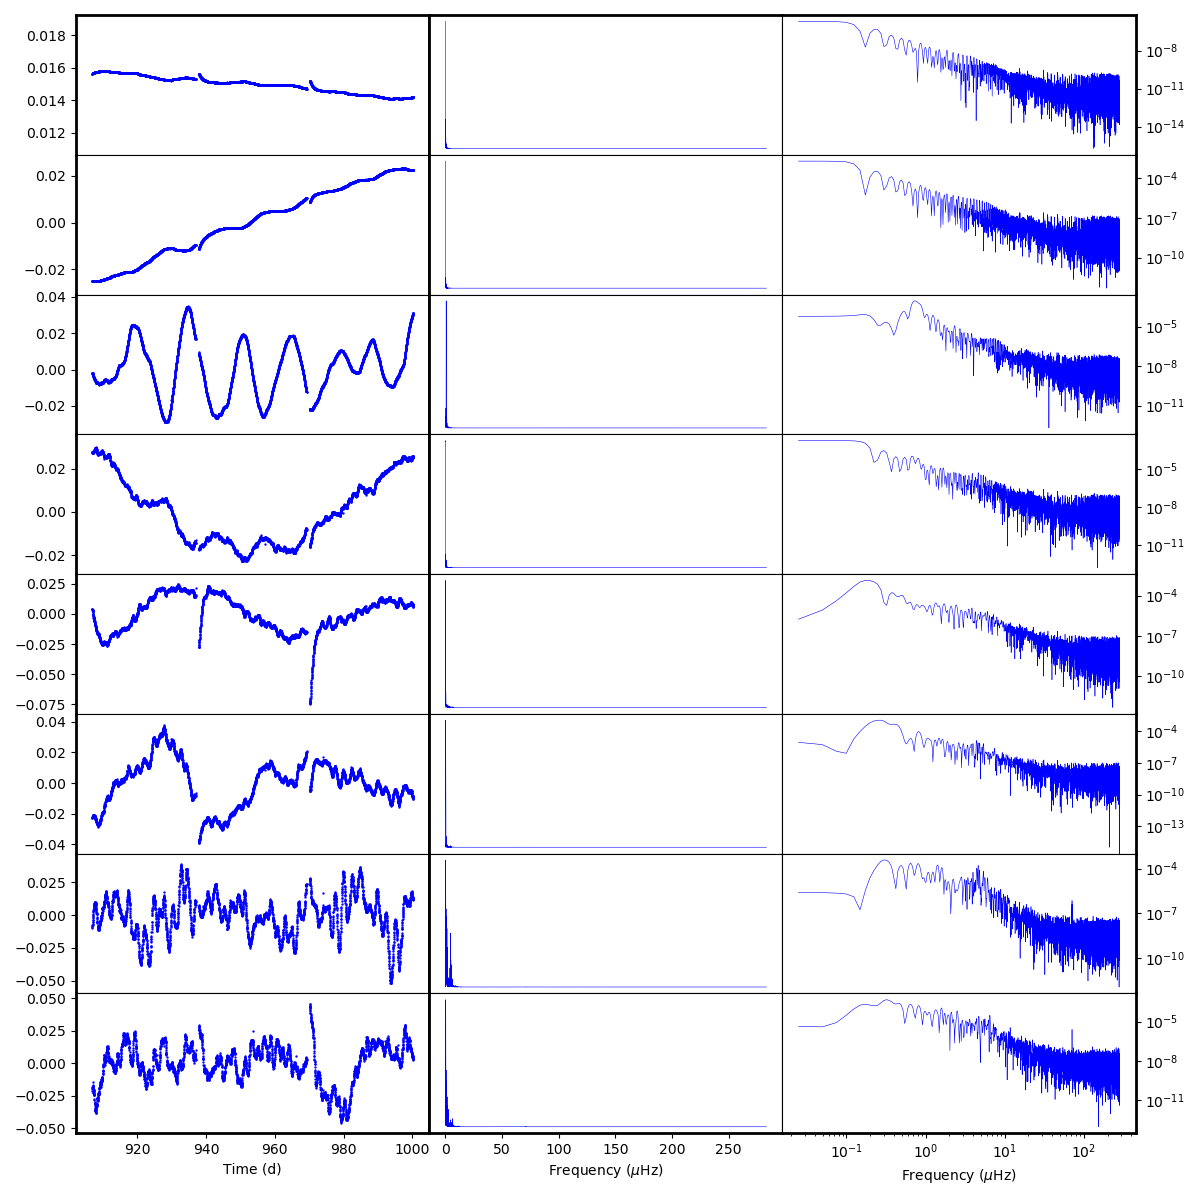
\includegraphics[width=\linewidth]{Chapter_Appended/AppB/cbv_6791_rgs_q10.png}
    \caption{Same as Figure \ref{fig:cbvs_rgsIS_6791_Q2} but for quarter 10.}
    \label{fig:cbvs_rgsIS_6791_Q10}
\end{figure}


\begin{figure}
    \centering
    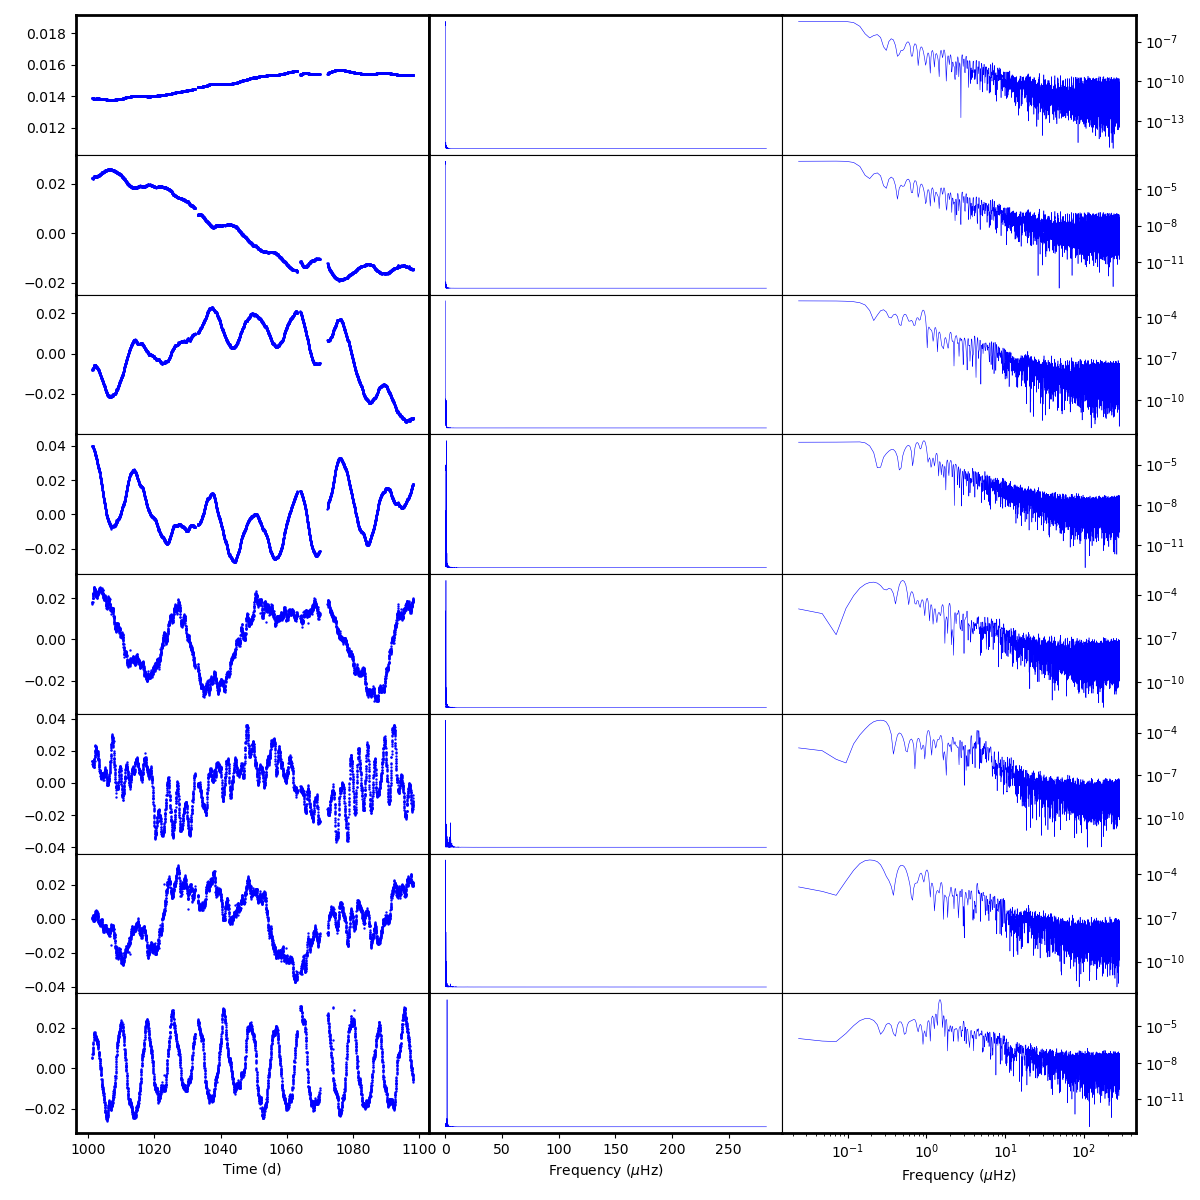
\includegraphics[width=\linewidth]{Chapter_Appended/AppB/cbv_6791_rgs_q11.png}
    \caption{Same as Figure \ref{fig:cbvs_rgsIS_6791_Q2} but for quarter 11.}
    \label{fig:cbvs_rgsIS_6791_Q11}
\end{figure}


\begin{figure}
    \centering
    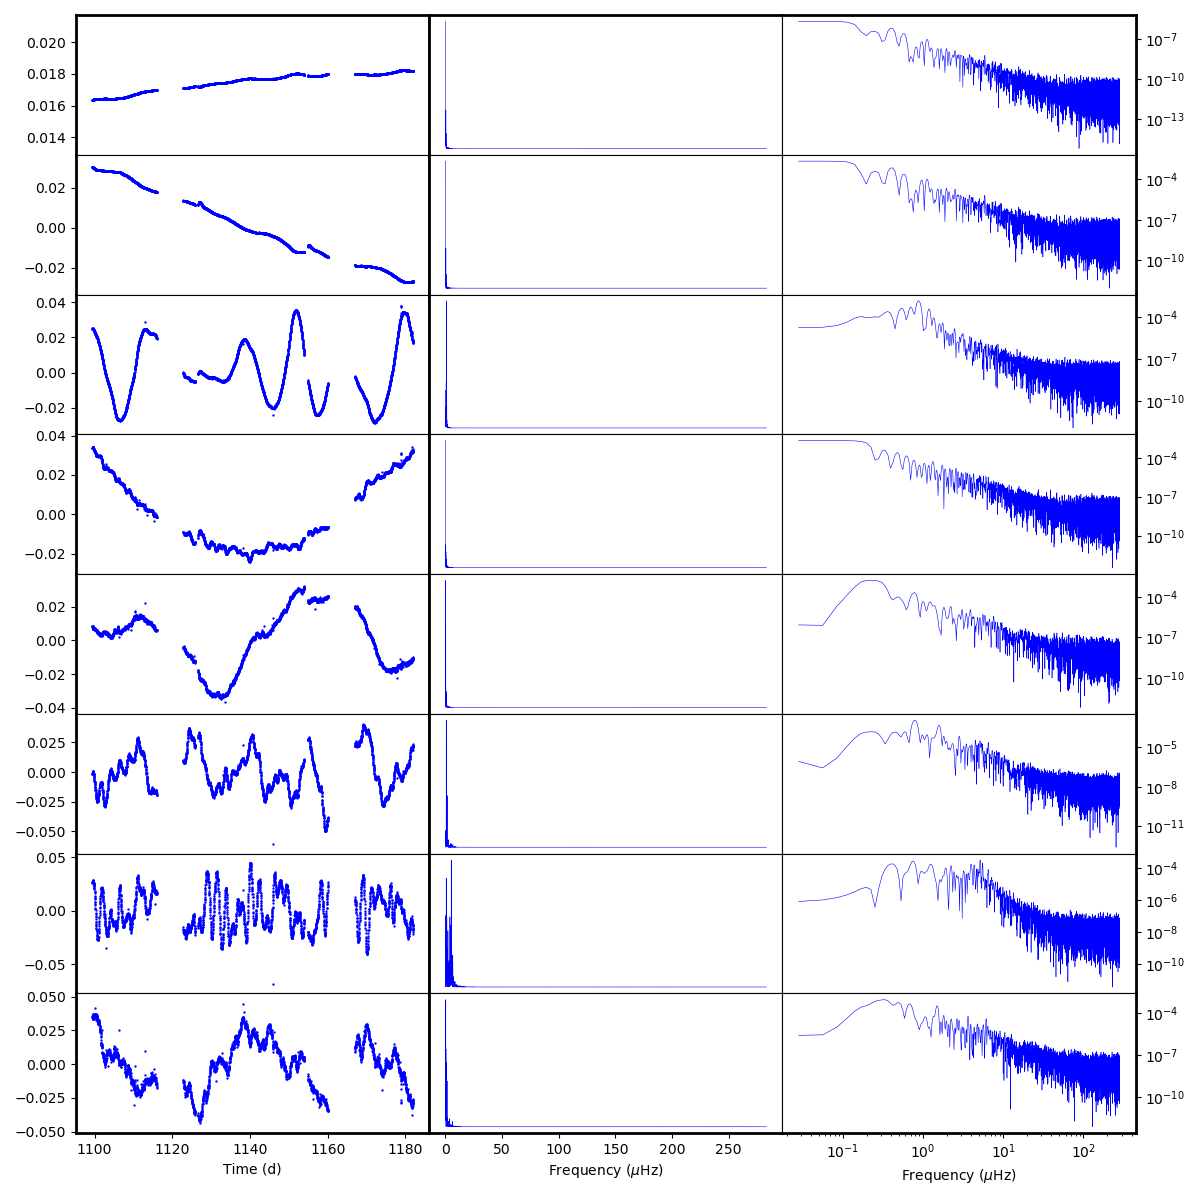
\includegraphics[width=\linewidth]{Chapter_Appended/AppB/cbv_6791_rgs_q12.png}
    \caption{Same as Figure \ref{fig:cbvs_rgsIS_6791_Q2} but for quarter 12.}
    \label{fig:cbvs_rgsIS_6791_Q12}
\end{figure}


\begin{figure}
    \centering
    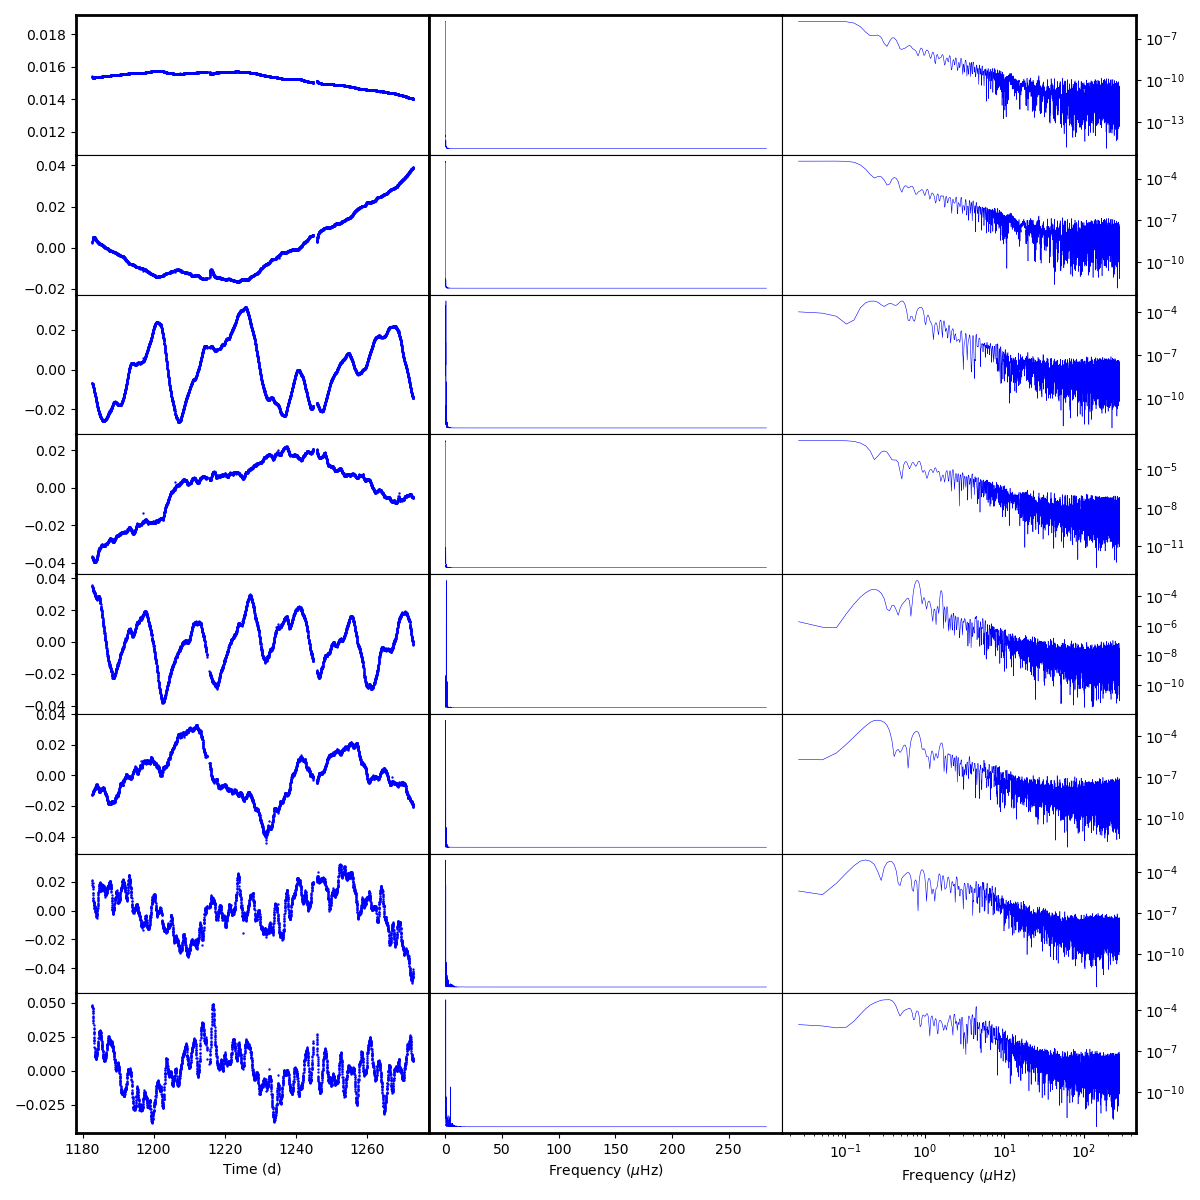
\includegraphics[width=\linewidth]{Chapter_Appended/AppB/cbv_6791_rgs_q13.png}
    \caption{Same as Figure \ref{fig:cbvs_rgsIS_6791_Q2} but for quarter 13.}
    \label{fig:cbvs_rgsIS_6791_Q13}
\end{figure}


\begin{figure}
    \centering
    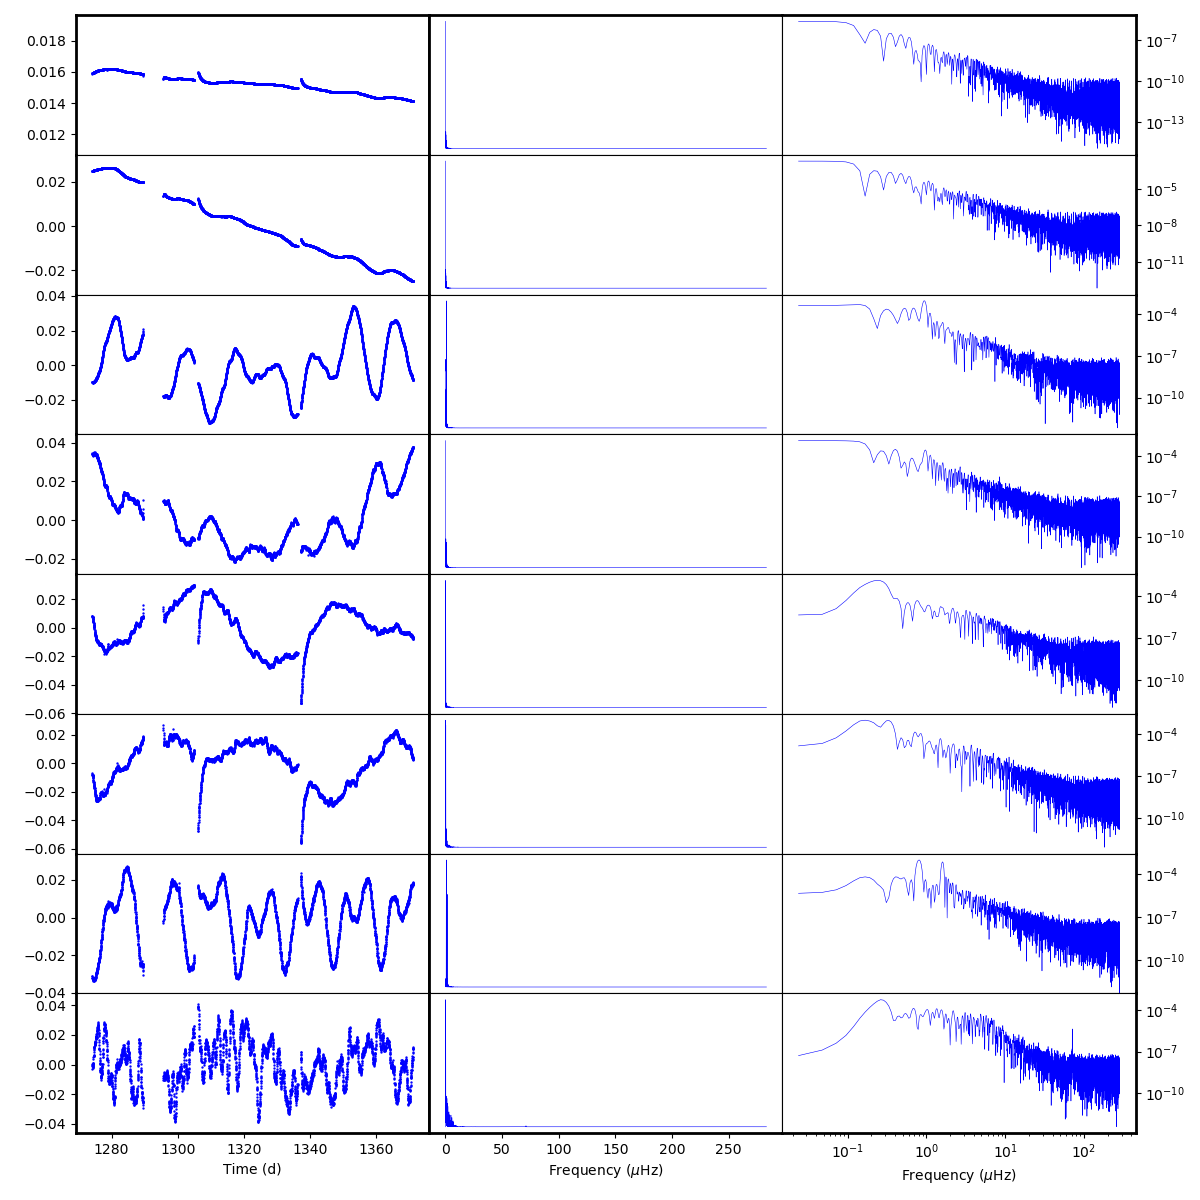
\includegraphics[width=\linewidth]{Chapter_Appended/AppB/cbv_6791_rgs_q14.png}
    \caption{Same as Figure \ref{fig:cbvs_rgsIS_6791_Q2} but for quarter 14.}
    \label{fig:cbvs_rgsIS_6791_Q14}
\end{figure}


\begin{figure}
    \centering
    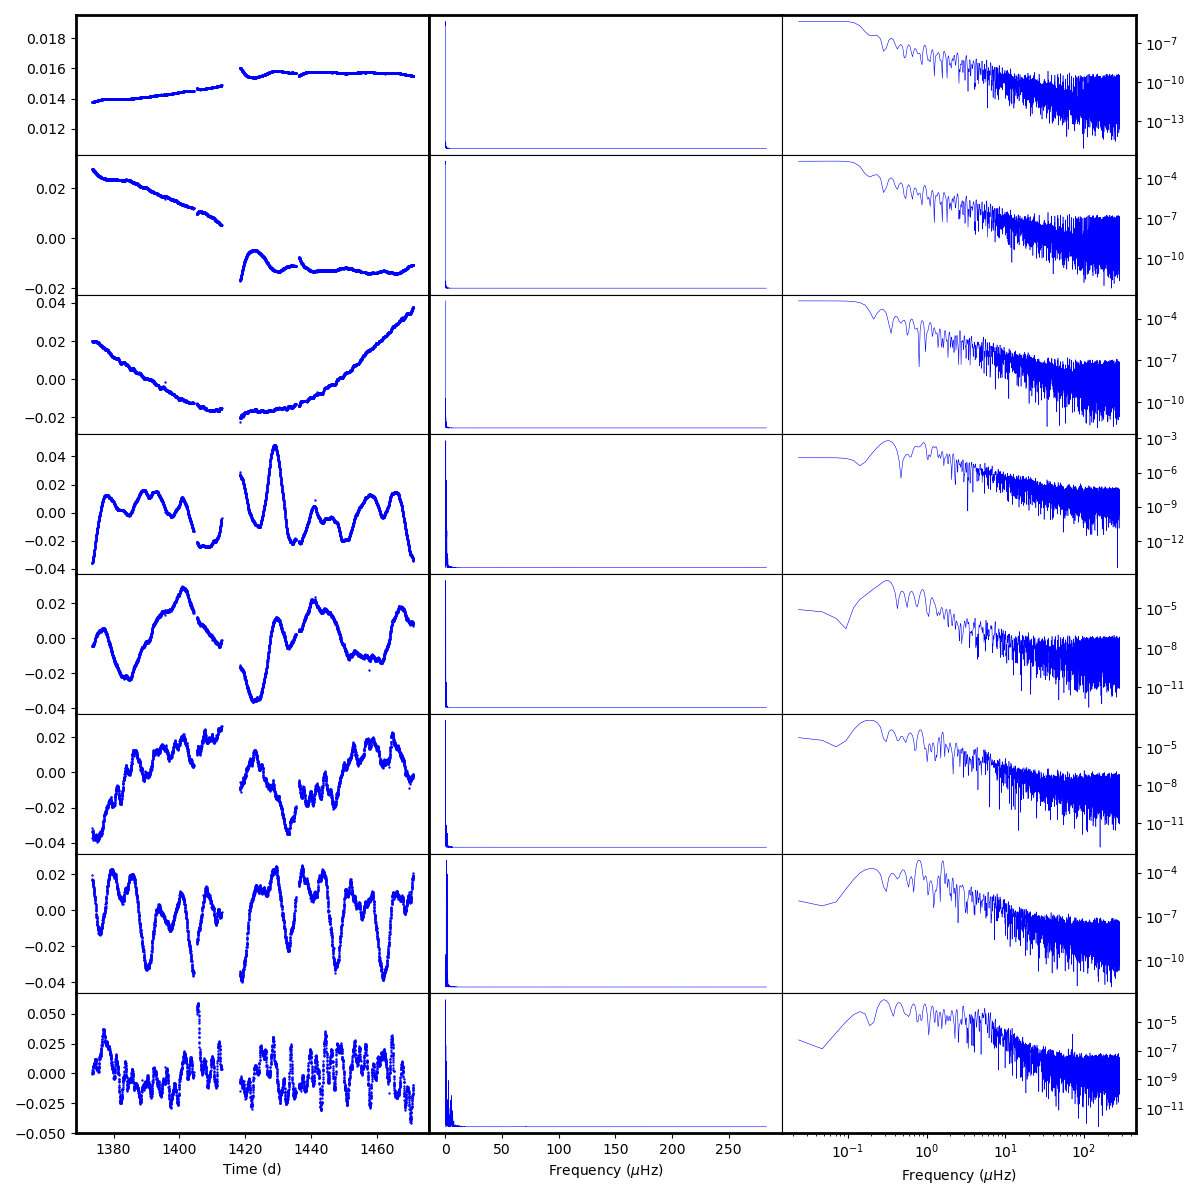
\includegraphics[width=\linewidth]{Chapter_Appended/AppB/cbv_6791_rgs_q15.png}
    \caption{Same as Figure \ref{fig:cbvs_rgsIS_6791_Q2} but for quarter 15.}
    \label{fig:cbvs_rgsIS_6791_Q15}
\end{figure}


\begin{figure}
    \centering
    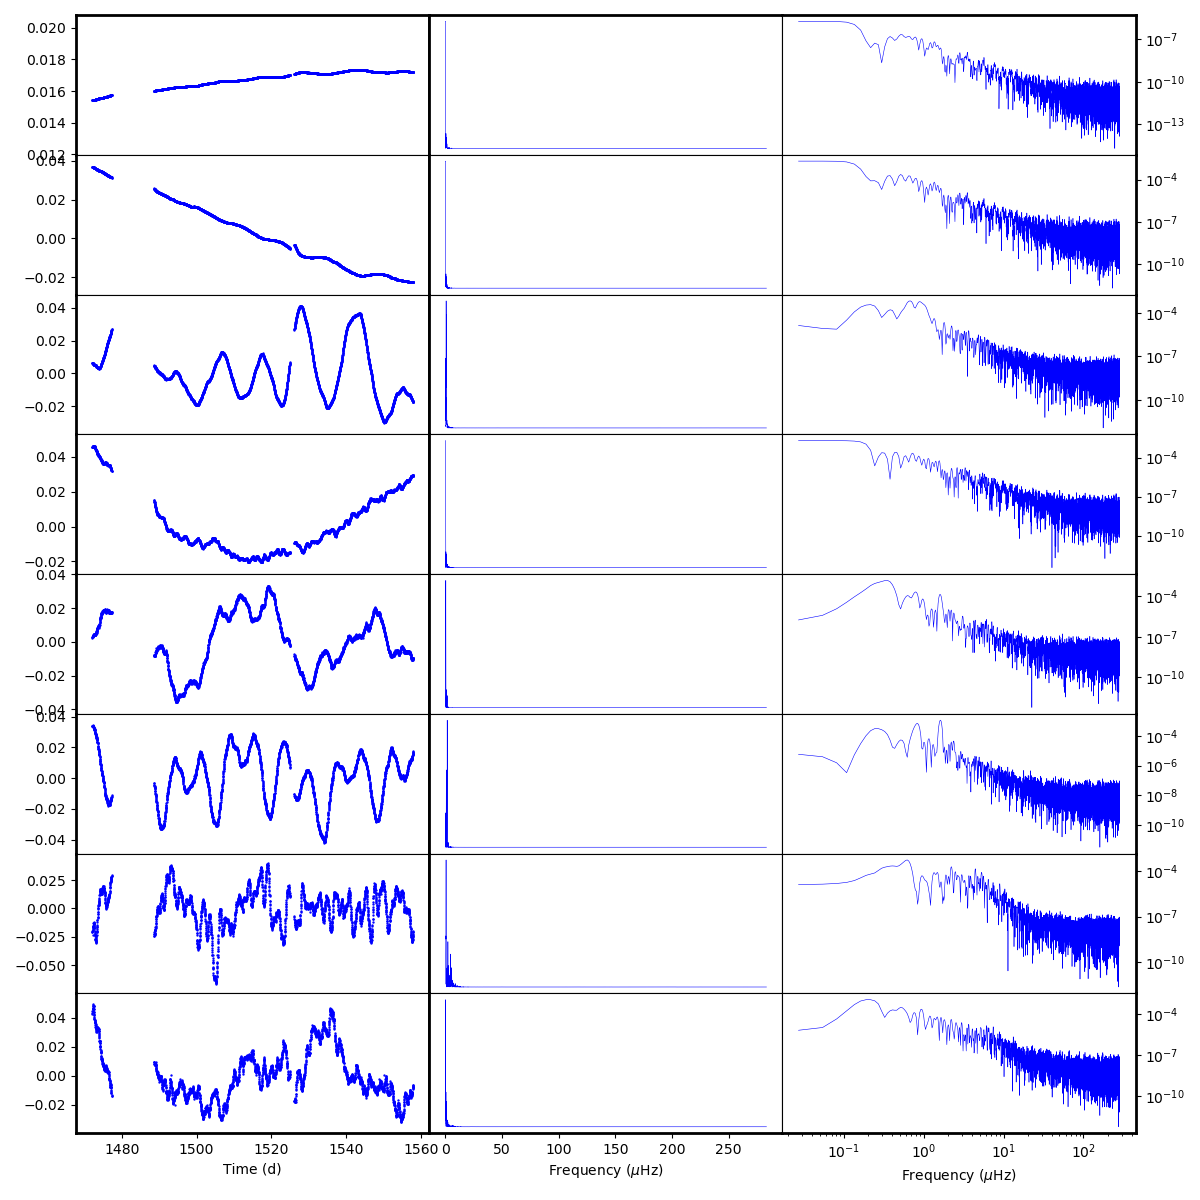
\includegraphics[width=\linewidth]{Chapter_Appended/AppB/cbv_6791_rgs_q16.png}
    \caption{Same as Figure \ref{fig:cbvs_rgsIS_6791_Q2} but for quarter 16.}
    \label{fig:cbvs_rgsIS_6791_Q16}
\end{figure}


\begin{figure}
    \centering
    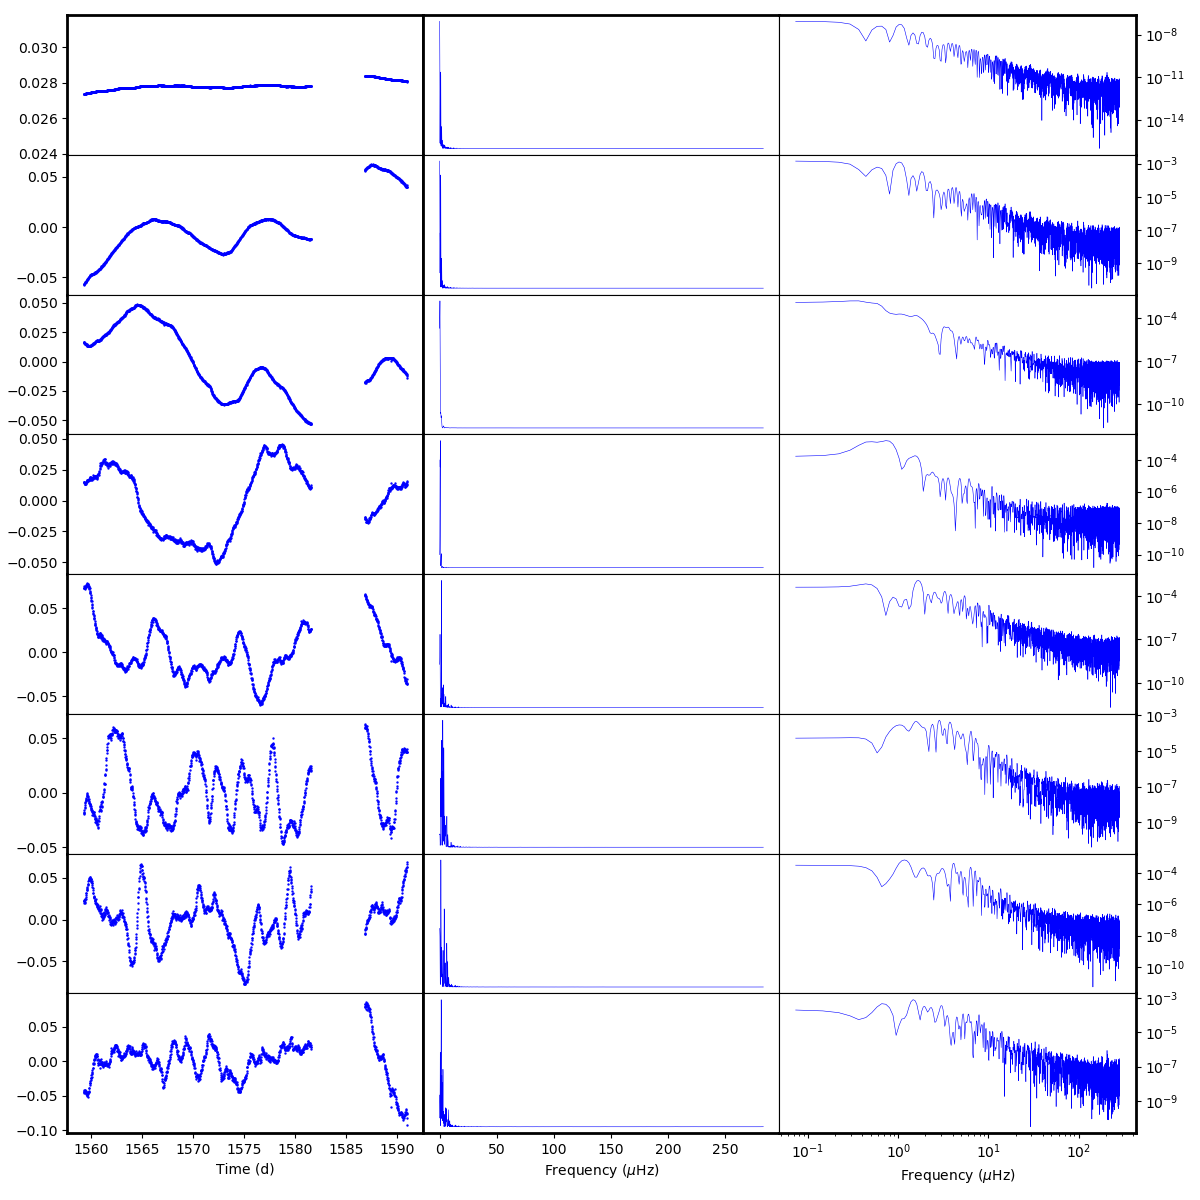
\includegraphics[width=\linewidth]{Chapter_Appended/AppB/cbv_6791_rgs_q17.png}
    \caption{Same as Figure \ref{fig:cbvs_rgsIS_6791_Q2} but for quarter 17.}
    \label{fig:cbvs_rgsIS_6791_Q17}
\end{figure}

\clearpage

\section*{NGC\,6819}
\begin{figure}[b]
    \centering
    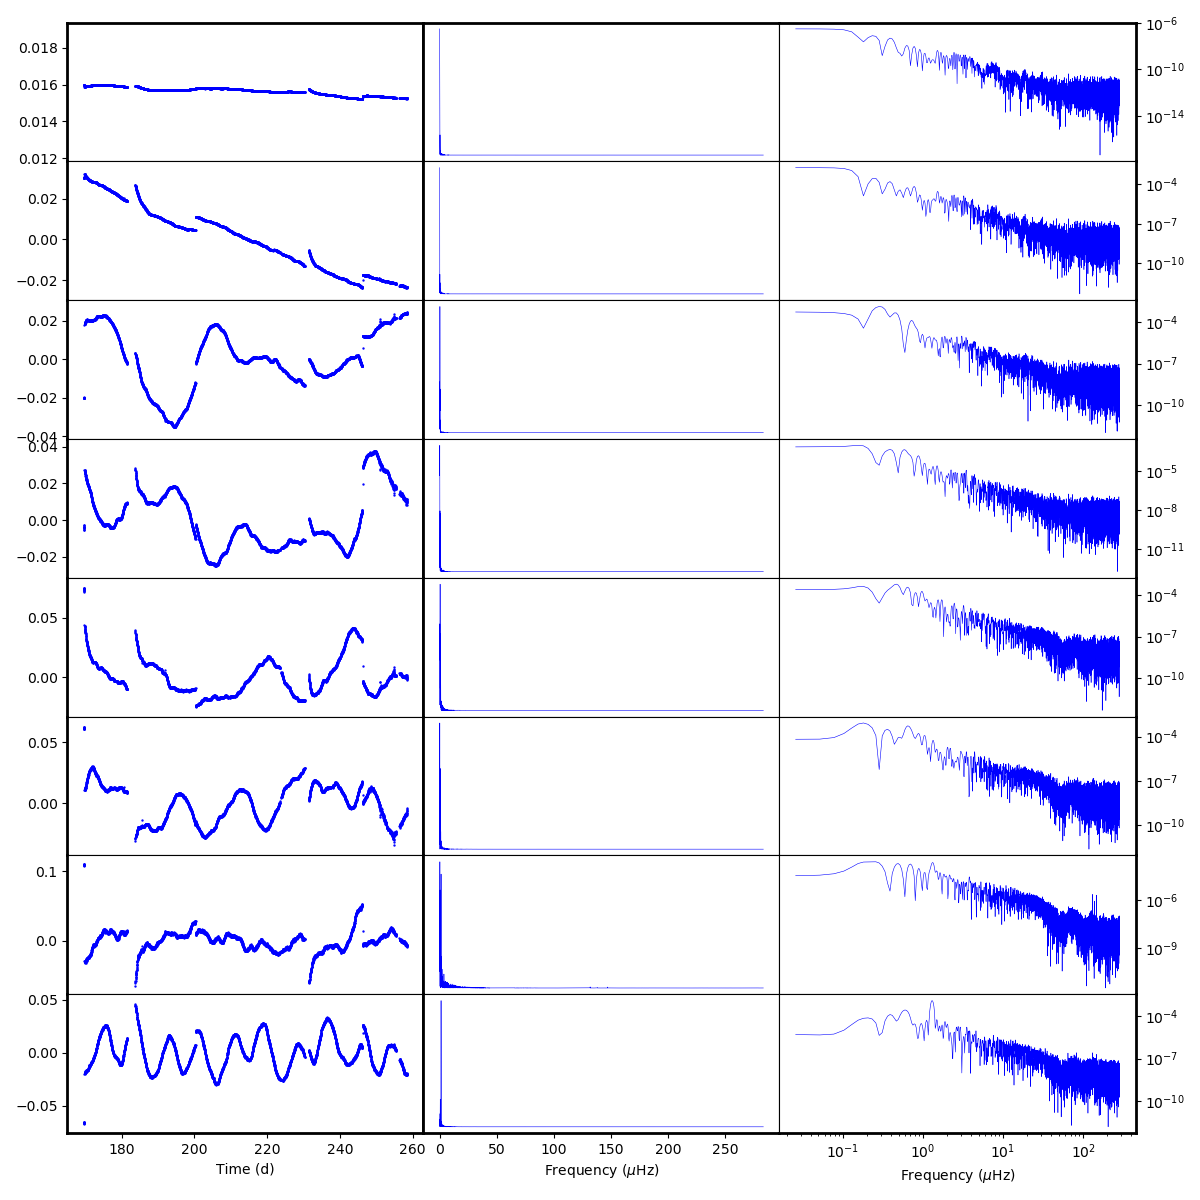
\includegraphics[width=\linewidth]{Chapter_Appended/AppB/cbv_6819_q02.png}
    \caption{The first 8 co-trending basis vectors (CBVs) for NGC\,6819 for the second data quarter (left), and the Fourier transform of these vectors (middle), and in log-log space (right) from the full set of image subtracted light curves.}
    \label{fig:cbvs_allIS_6819_Q2}
\end{figure}


\begin{figure}
    \centering
    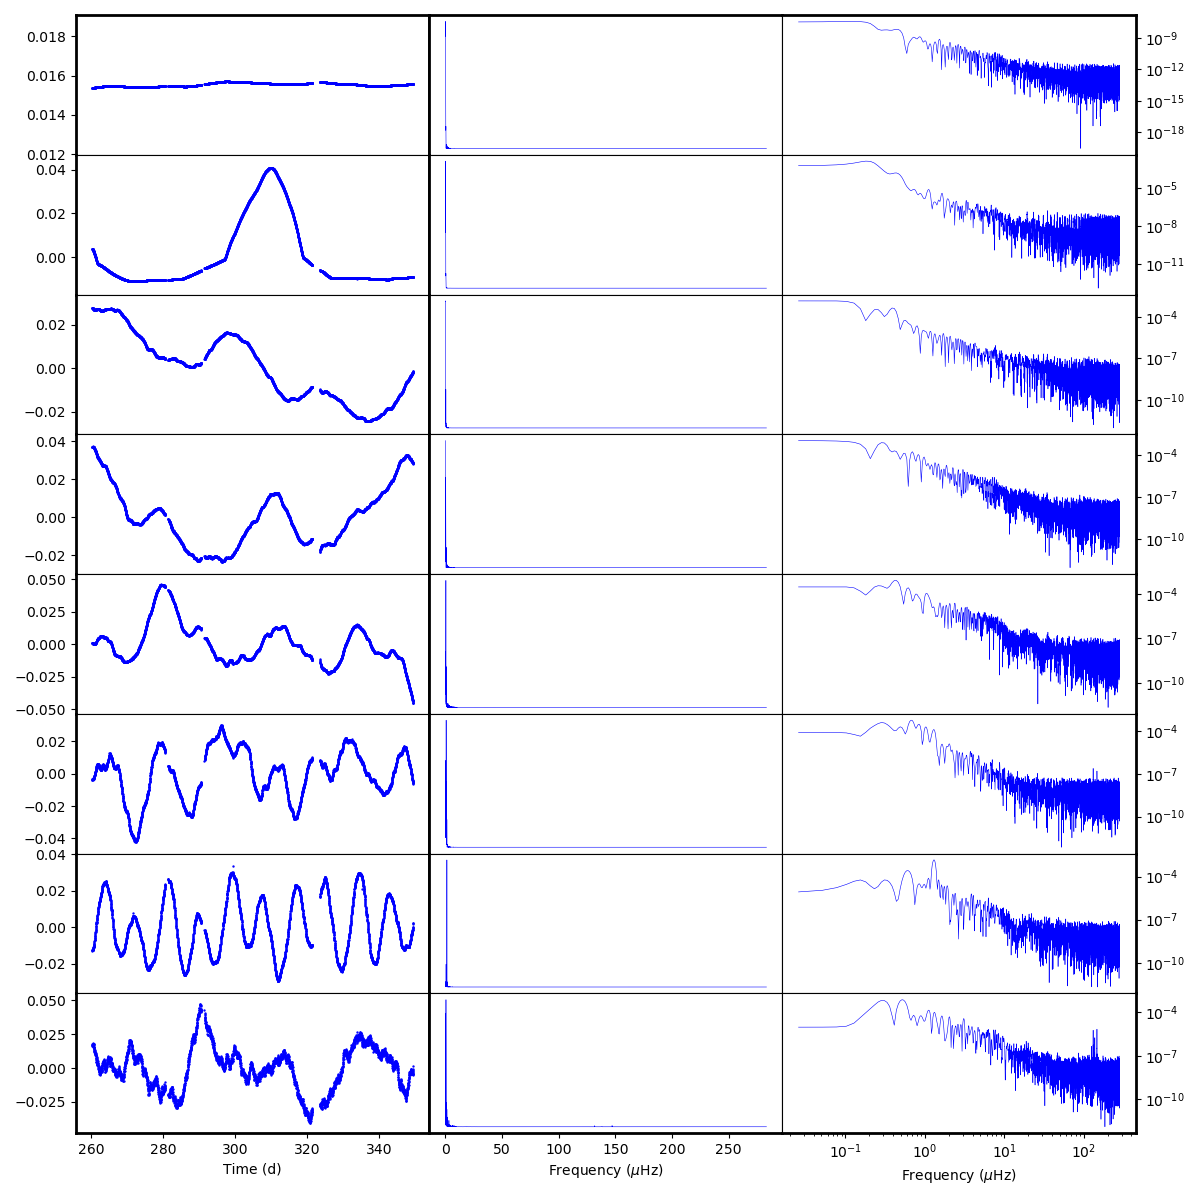
\includegraphics[width=\linewidth]{Chapter_Appended/AppB/cbv_6819_q03.png}
    \caption{Same as Figure \ref{fig:cbvs_allIS_6819_Q2} but for quarter 3.}
    \label{fig:cbvs_allIS_6819_Q03}
\end{figure}


\begin{figure}
    \centering
    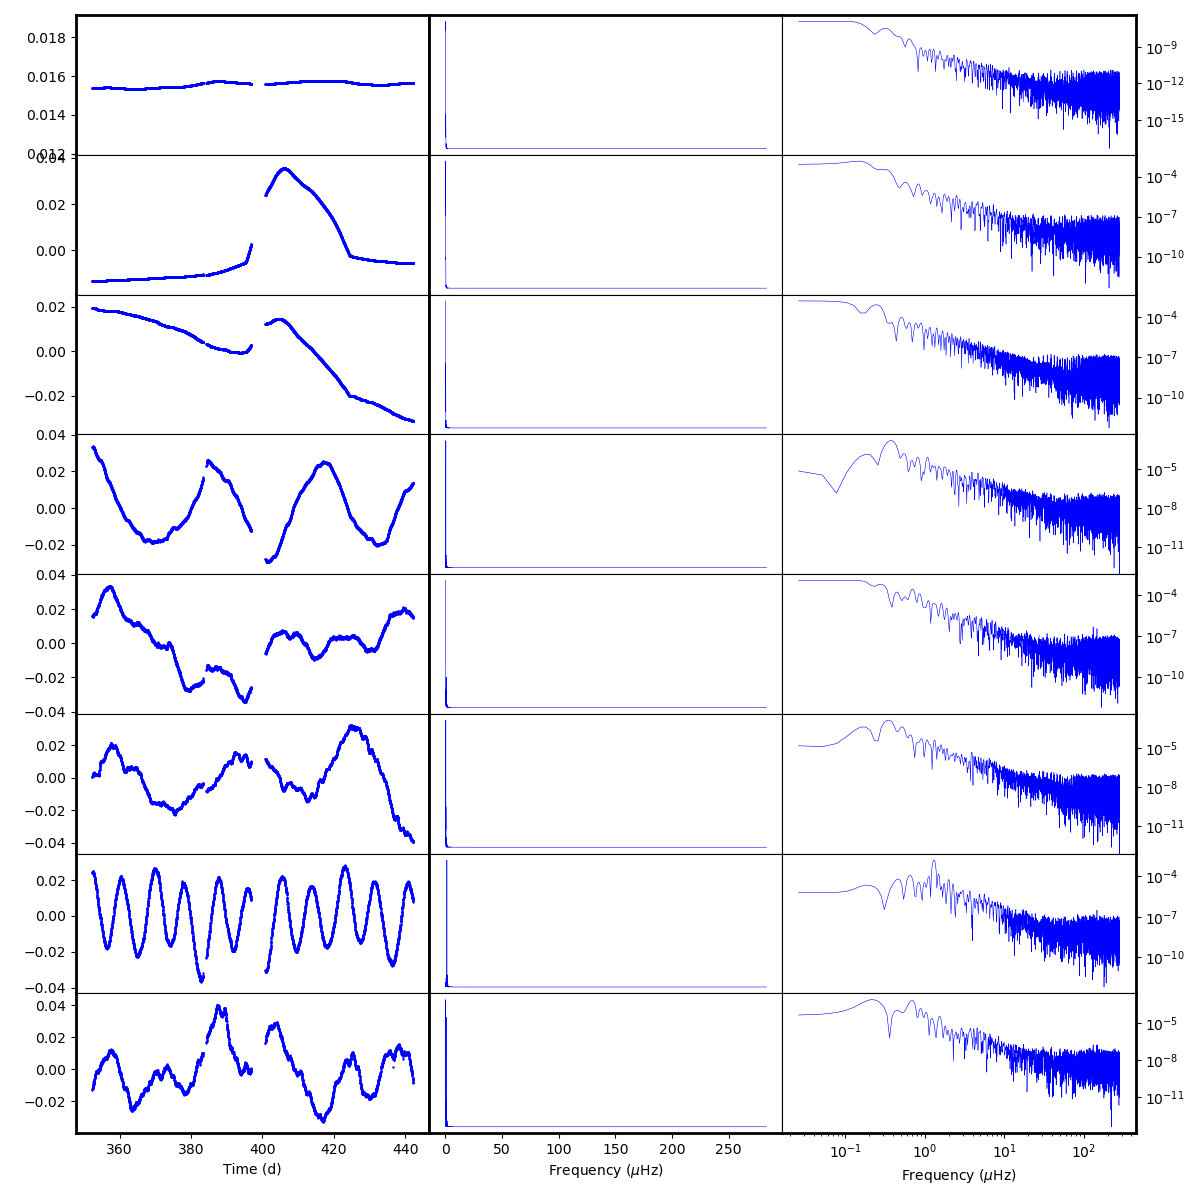
\includegraphics[width=\linewidth]{Chapter_Appended/AppB/cbv_6819_q04.png}
    \caption{Same as Figure \ref{fig:cbvs_allIS_6819_Q2} but for quarter 4.}
    \label{fig:cbvs_allIS_6819_Q04}
\end{figure}


\begin{figure}
    \centering
    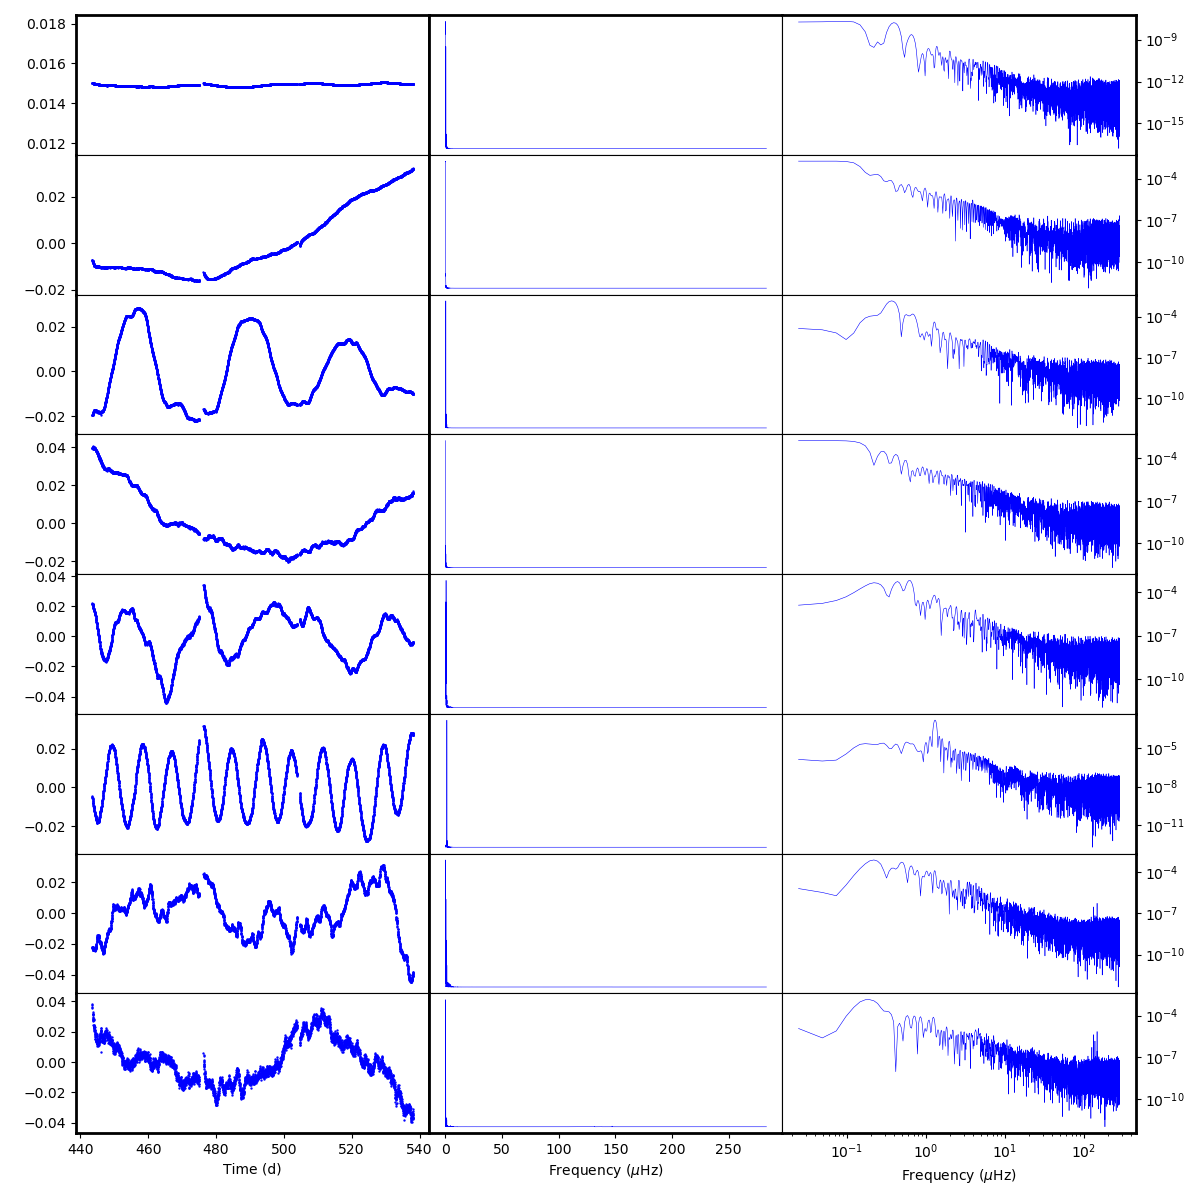
\includegraphics[width=\linewidth]{Chapter_Appended/AppB/cbv_6819_q05.png}
    \caption{Same as Figure \ref{fig:cbvs_allIS_6819_Q2} but for quarter 5.}
    \label{fig:cbvs_allIS_6819_Q05}
\end{figure}


\begin{figure}
    \centering
    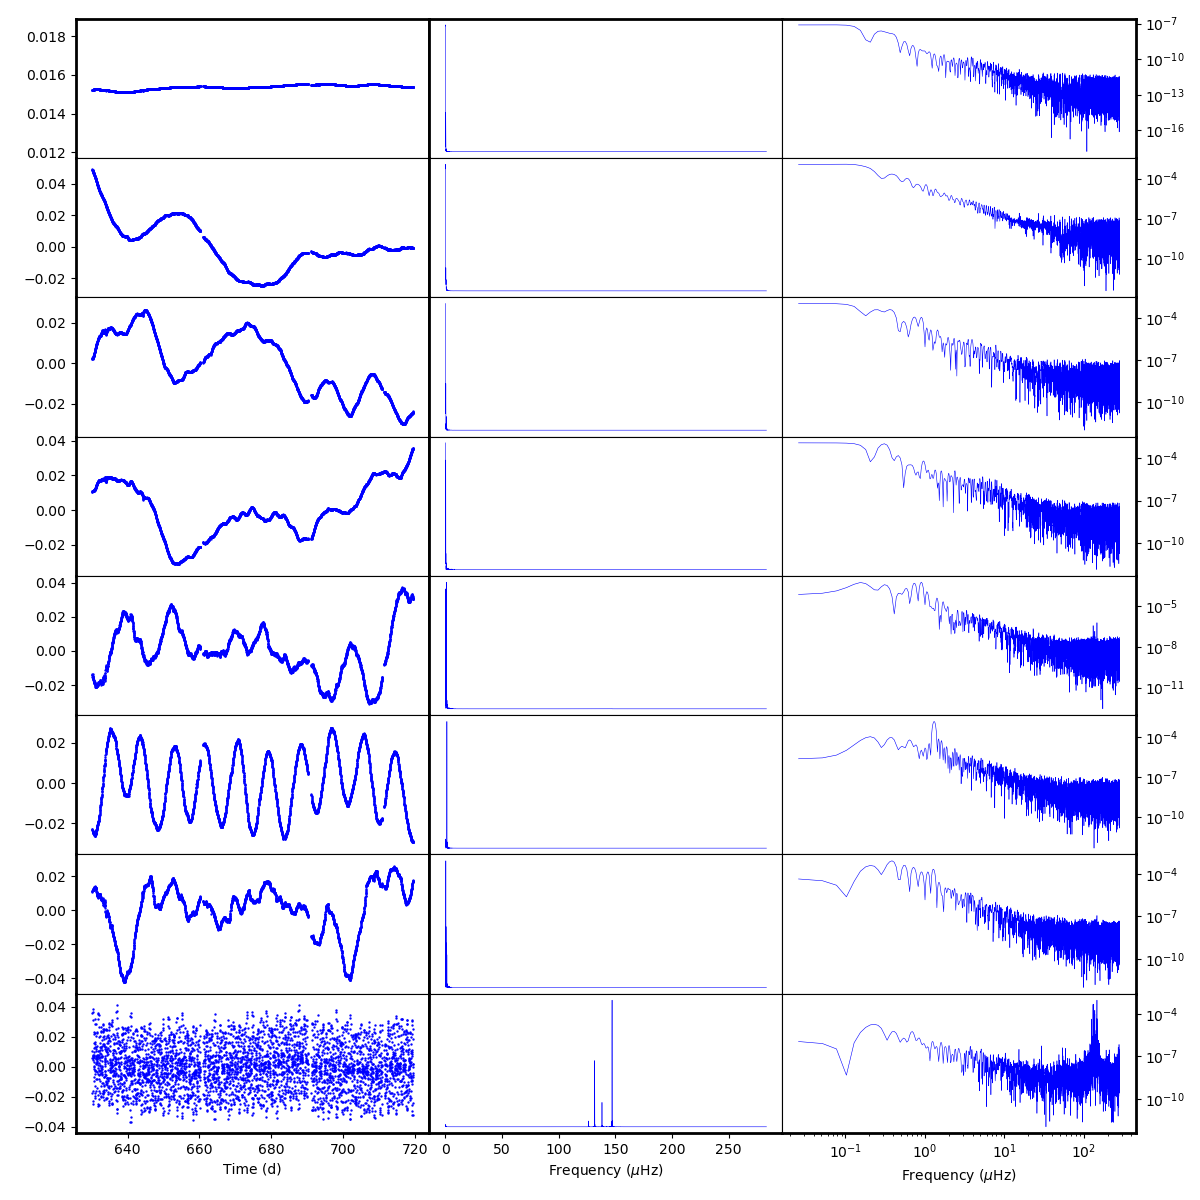
\includegraphics[width=\linewidth]{Chapter_Appended/AppB/cbv_6819_q07.png}
    \caption{Same as Figure \ref{fig:cbvs_allIS_6819_Q2} but for quarter 7.}
    \label{fig:cbvs_allIS_6819_Q07}
\end{figure}


\begin{figure}
    \centering
    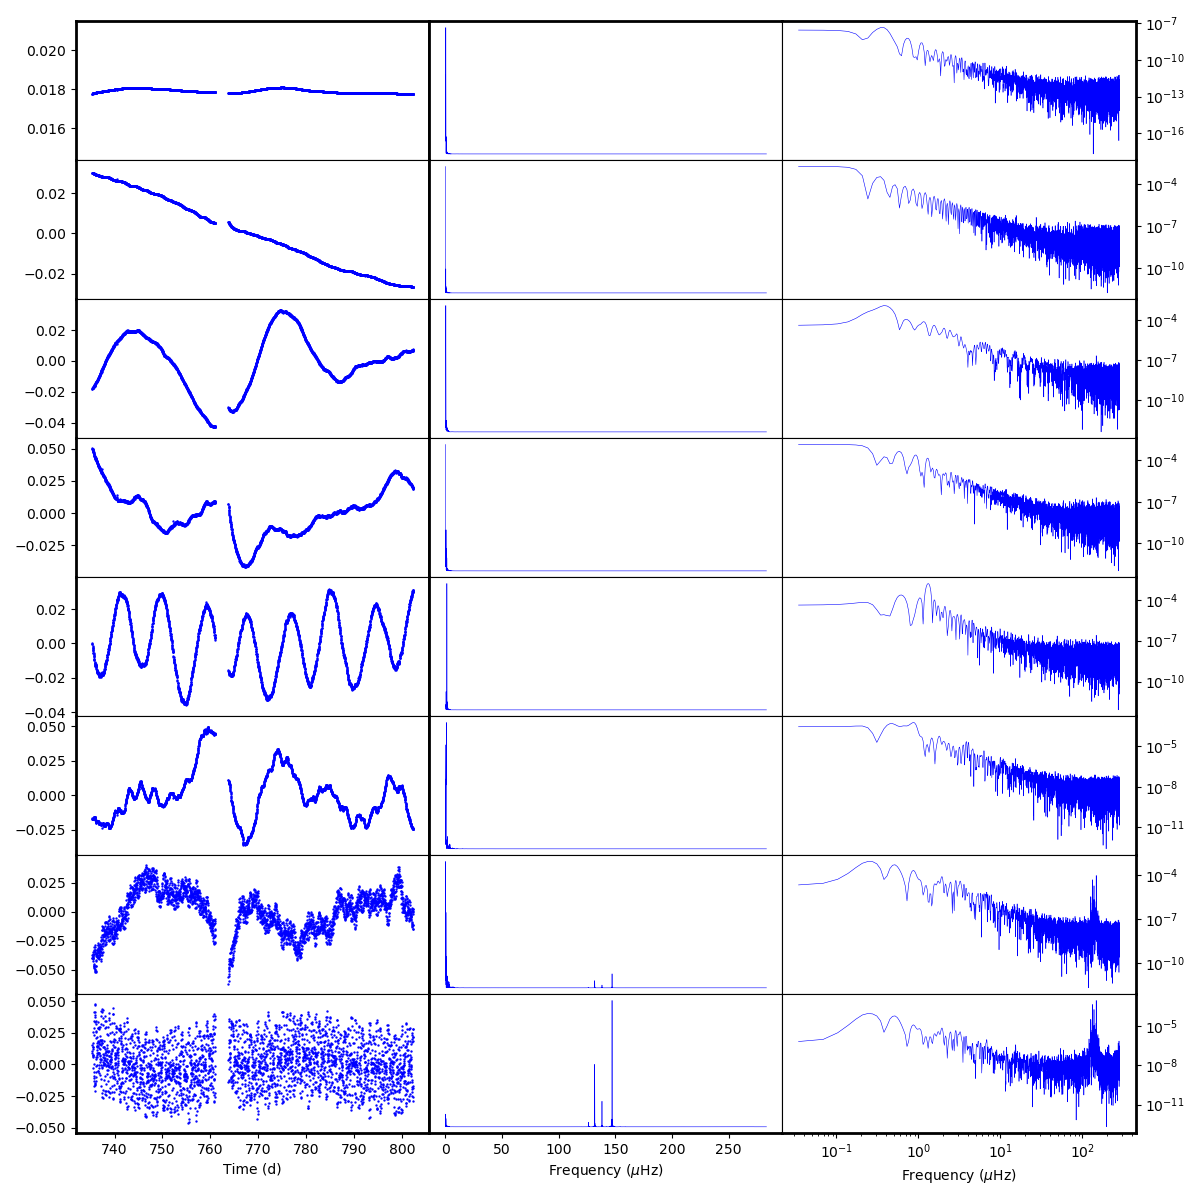
\includegraphics[width=\linewidth]{Chapter_Appended/AppB/cbv_6819_q08.png}
    \caption{Same as Figure \ref{fig:cbvs_allIS_6819_Q2} but for quarter 8.}
    \label{fig:cbvs_allIS_6819_Q08}
\end{figure}


\begin{figure}
    \centering
    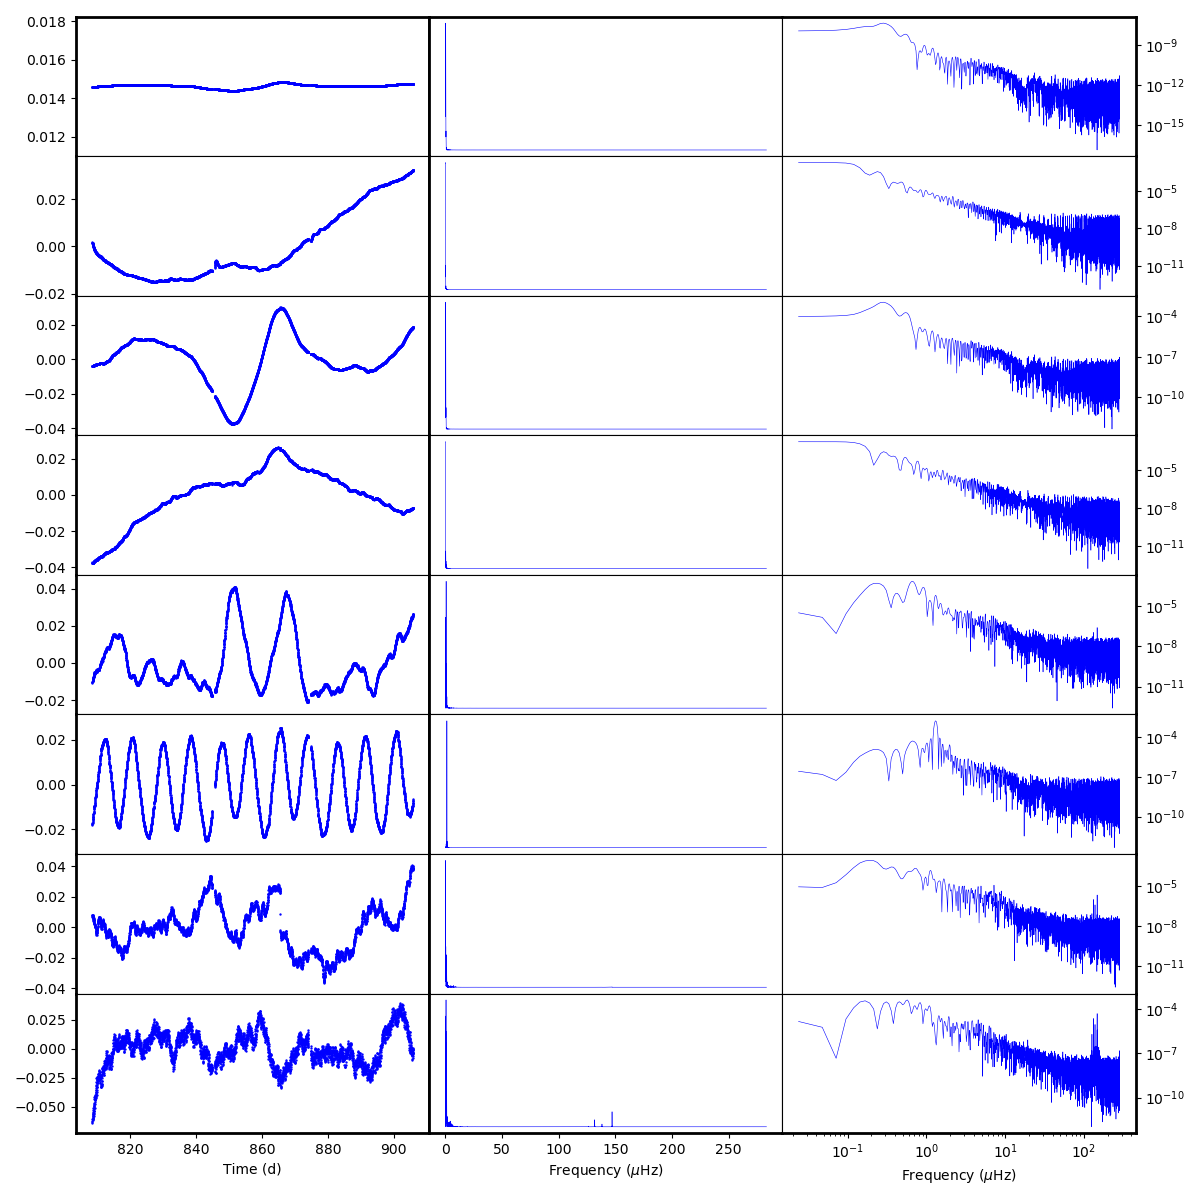
\includegraphics[width=\linewidth]{Chapter_Appended/AppB/cbv_6819_q09.png}
    \caption{Same as Figure \ref{fig:cbvs_allIS_6819_Q2} but for quarter 9.}
    \label{fig:cbvs_allIS_6819_Q09}
\end{figure}


\begin{figure}
    \centering
    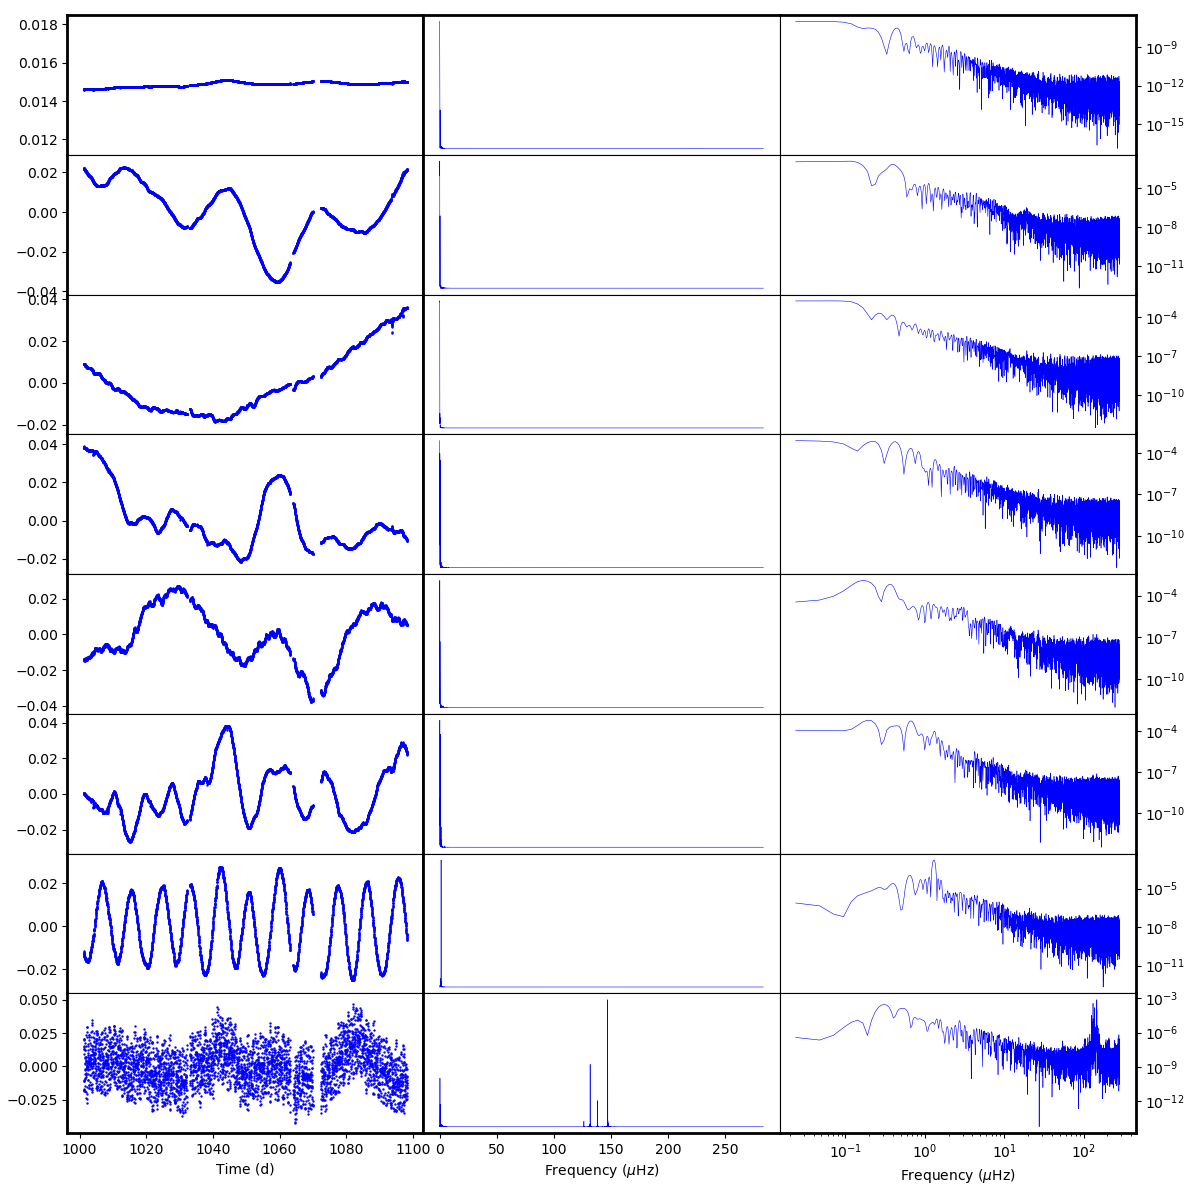
\includegraphics[width=\linewidth]{Chapter_Appended/AppB/cbv_6819_q11.png}
    \caption{Same as Figure \ref{fig:cbvs_allIS_6819_Q2} but for quarter 11.}
    \label{fig:cbvs_allIS_6819_Q11}
\end{figure}


\begin{figure}
    \centering
    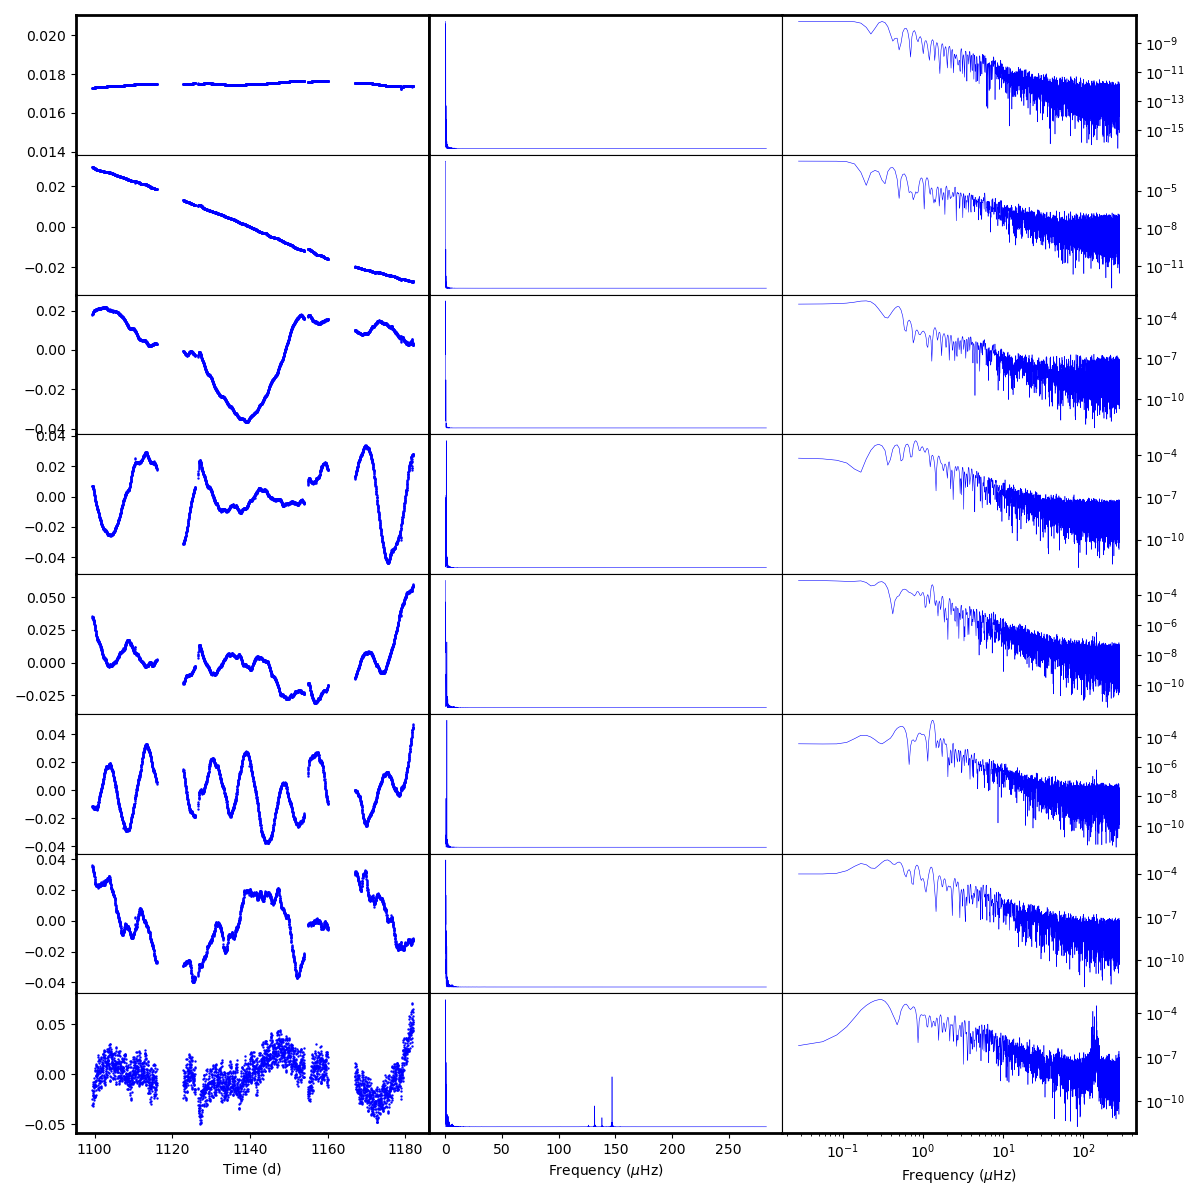
\includegraphics[width=\linewidth]{Chapter_Appended/AppB/cbv_6819_q12.png}
    \caption{Same as Figure \ref{fig:cbvs_allIS_6819_Q2} but for quarter 12.}
    \label{fig:cbvs_allIS_6819_Q12}
\end{figure}


\begin{figure}
    \centering
    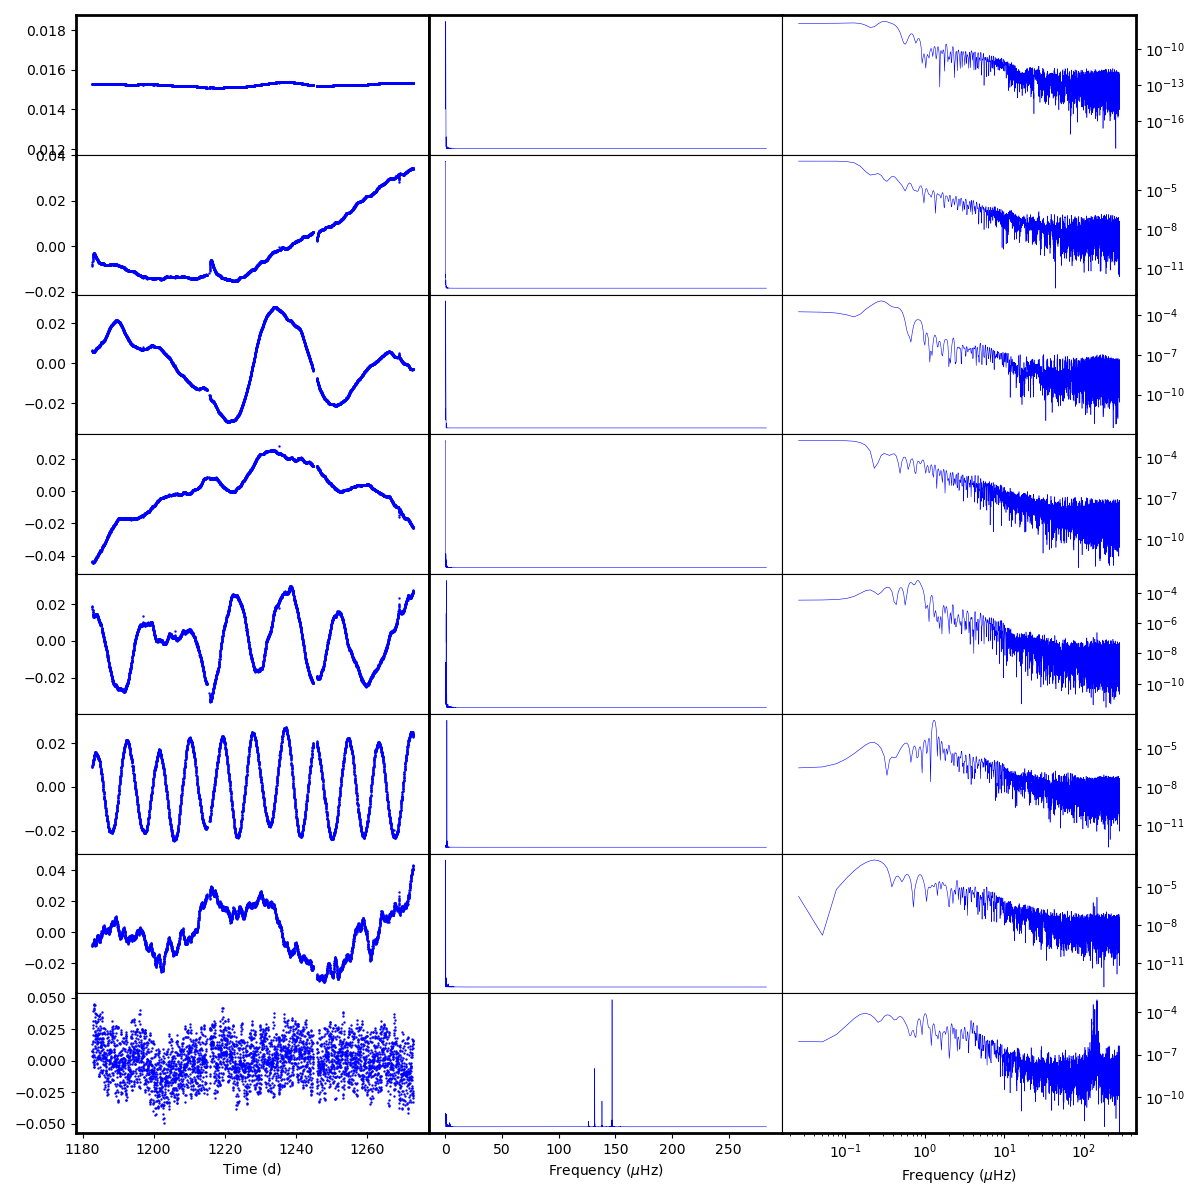
\includegraphics[width=\linewidth]{Chapter_Appended/AppB/cbv_6819_q13.png}
    \caption{Same as Figure \ref{fig:cbvs_allIS_6819_Q2} but for quarter 13.}
    \label{fig:cbvs_allIS_6819_Q13}
\end{figure}


\begin{figure}
    \centering
    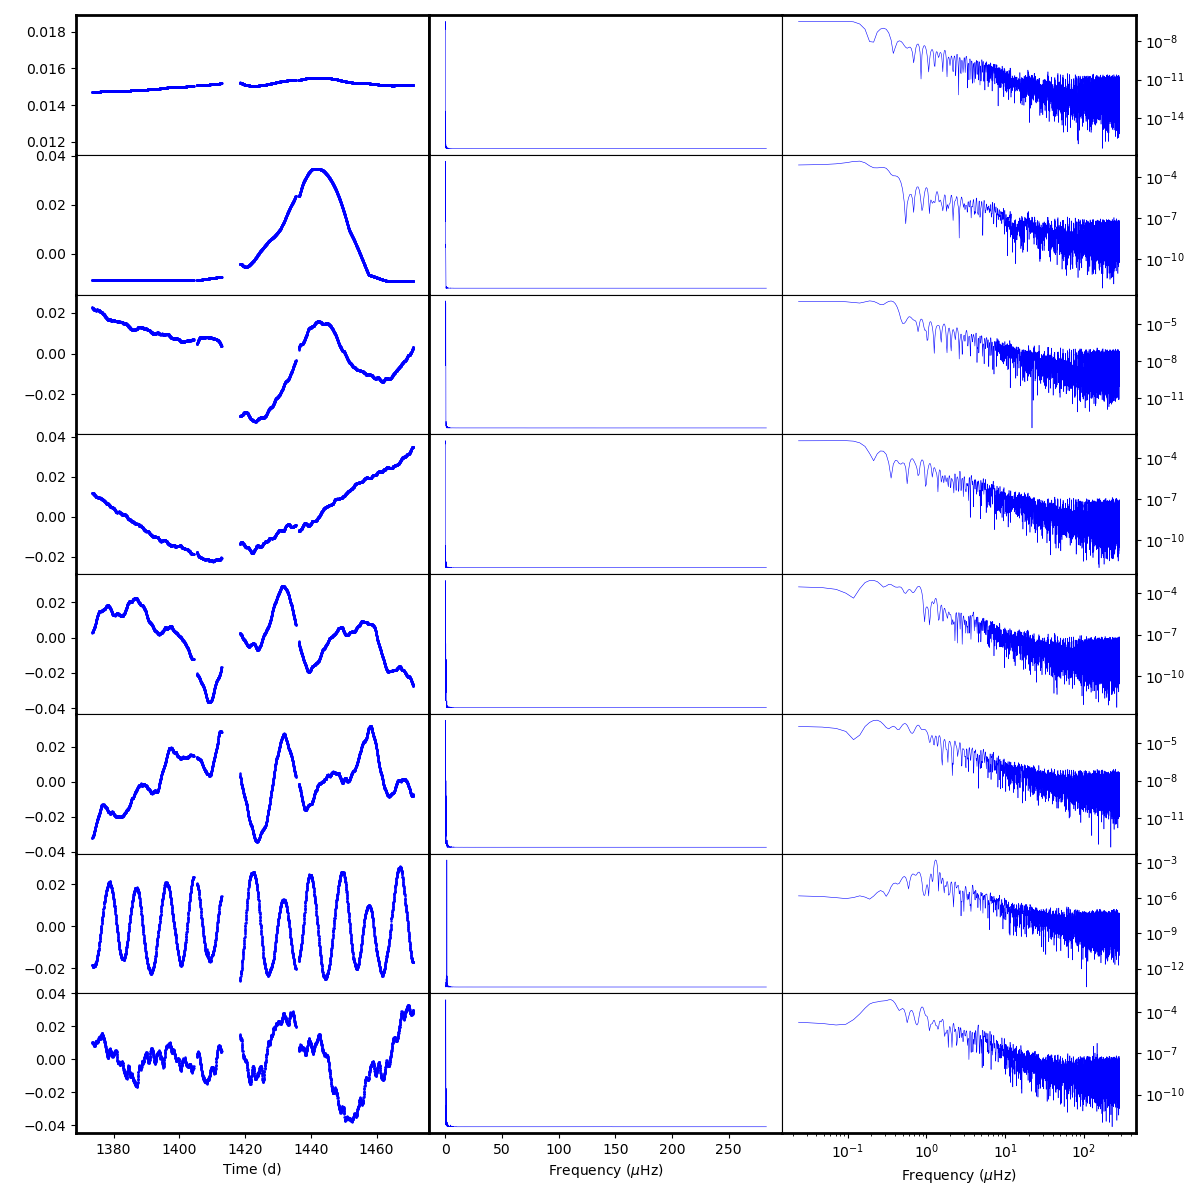
\includegraphics[width=\linewidth]{Chapter_Appended/AppB/cbv_6819_q15.png}
    \caption{Same as Figure \ref{fig:cbvs_allIS_6819_Q2} but for quarter 15.}
    \label{fig:cbvs_allIS_6819_Q15}
\end{figure}


\begin{figure}
    \centering
    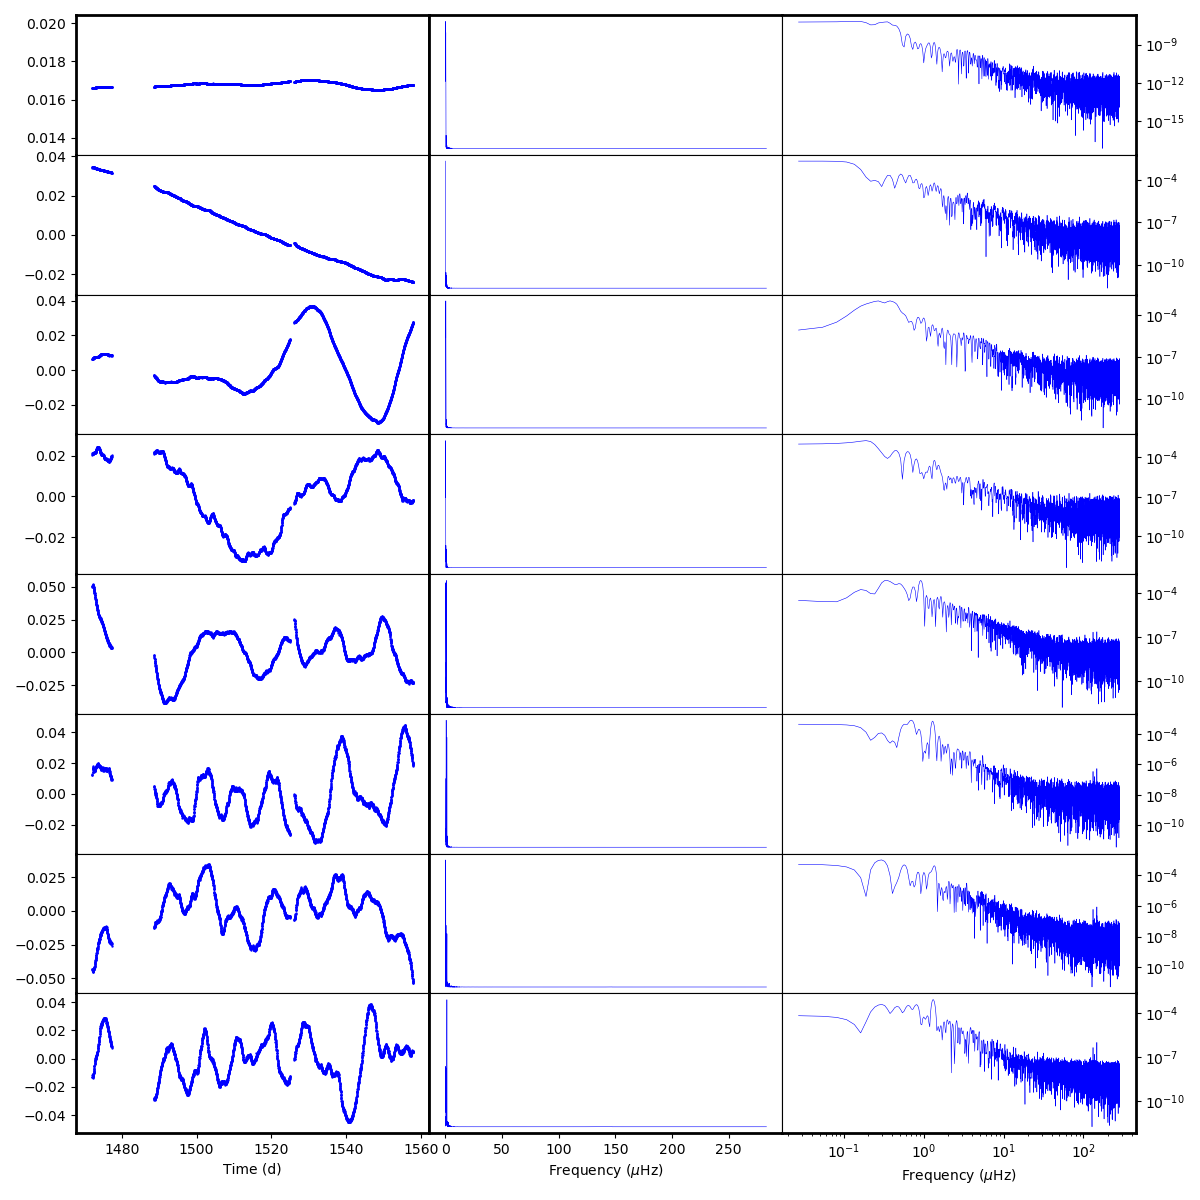
\includegraphics[width=\linewidth]{Chapter_Appended/AppB/cbv_6819_q16.png}
    \caption{Same as Figure \ref{fig:cbvs_allIS_6819_Q2} but for quarter 16.}
    \label{fig:cbvs_allIS_6819_Q16}
\end{figure}


\begin{figure}
    \centering
    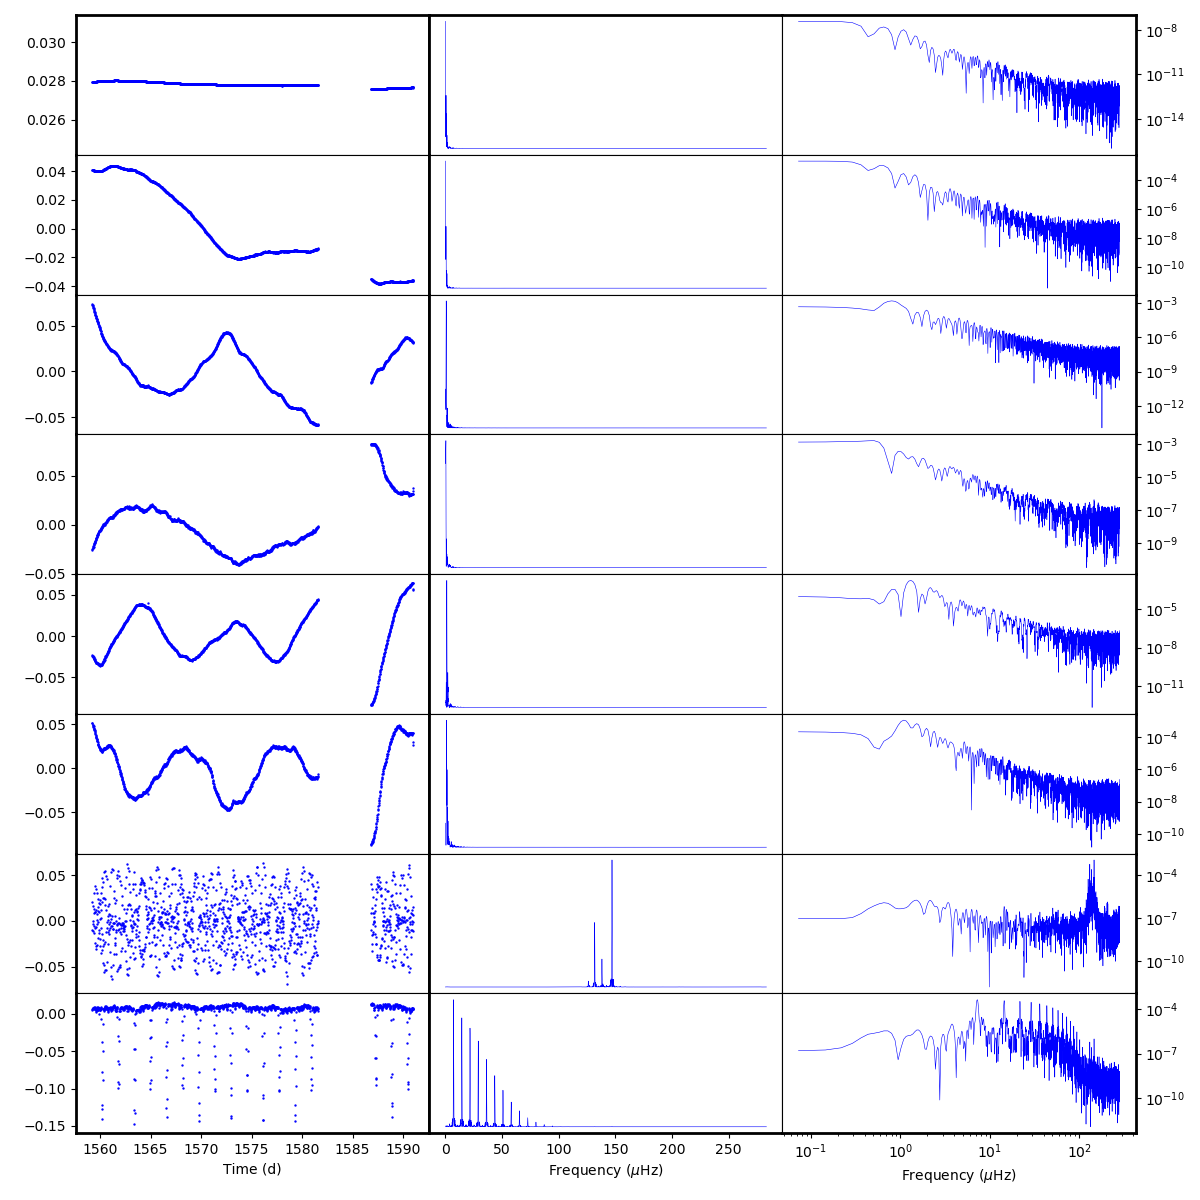
\includegraphics[width=\linewidth]{Chapter_Appended/AppB/cbv_6819_q17.png}
    \caption{Same as Figure \ref{fig:cbvs_allIS_6819_Q2} but for quarter 17.}
    \label{fig:cbvs_allIS_6819_Q17}
\end{figure}


\begin{figure}
    \centering
    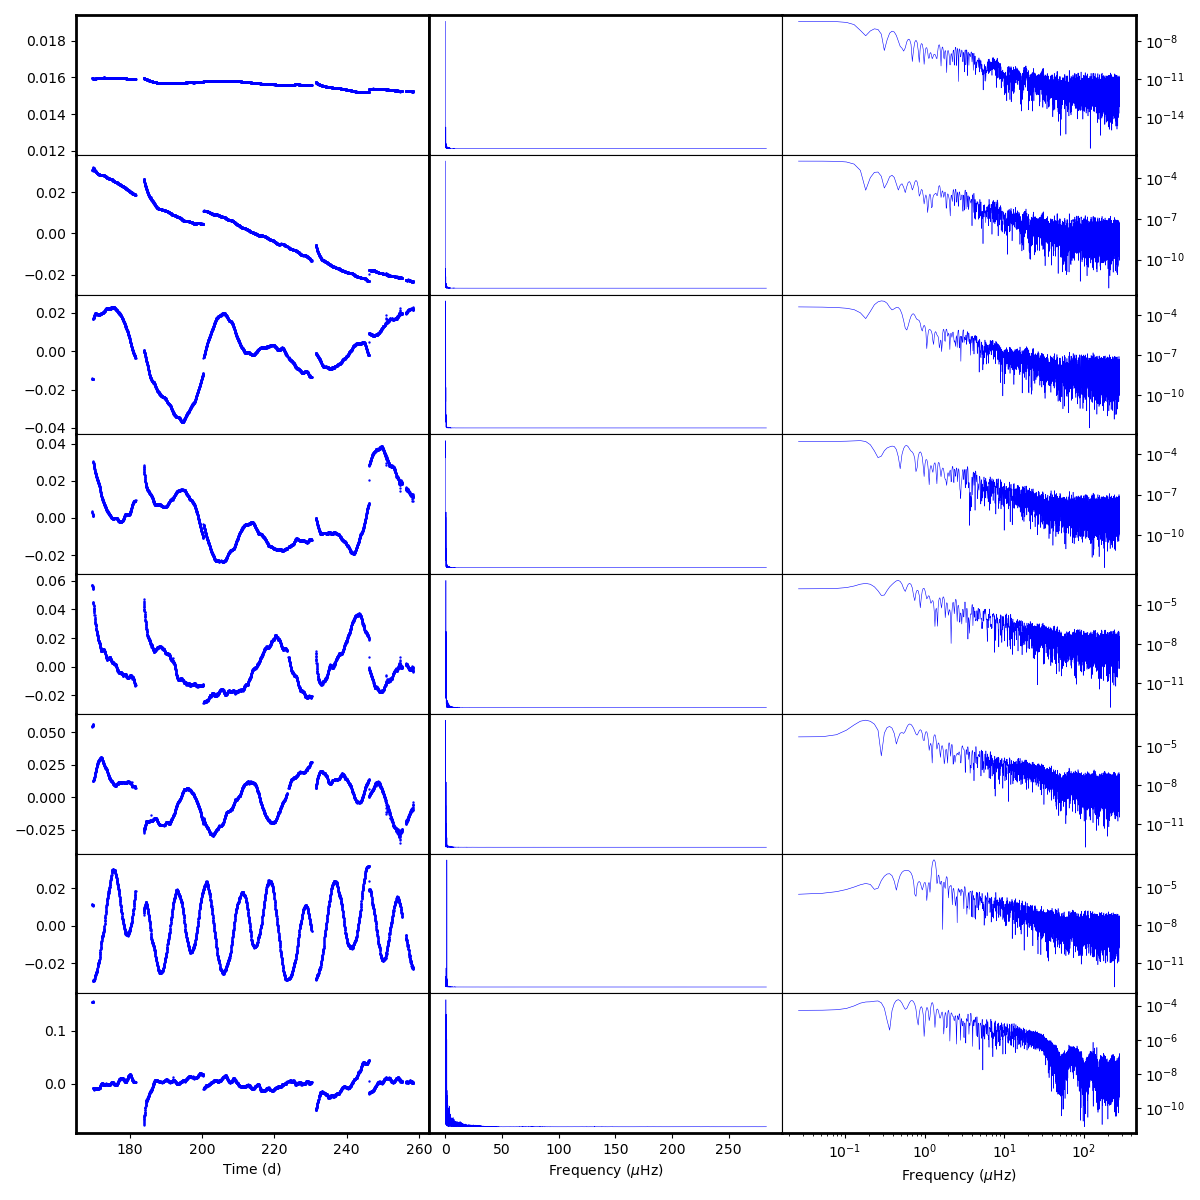
\includegraphics[width=\linewidth]{Chapter_Appended/AppB/cbv_6819_rgs_q02.png}
    \caption{The first 8 co-trending basis vectors (CBVs) for NGC\,6819 for the second data quarter (left), and the Fourier transform of these vectors (middle), and in log-log space (right) from the likely red giant member subset of image subtracted light curves.}
    \label{fig:cbvs_rgsIS_6819_Q2}
\end{figure}


\begin{figure}
    \centering
    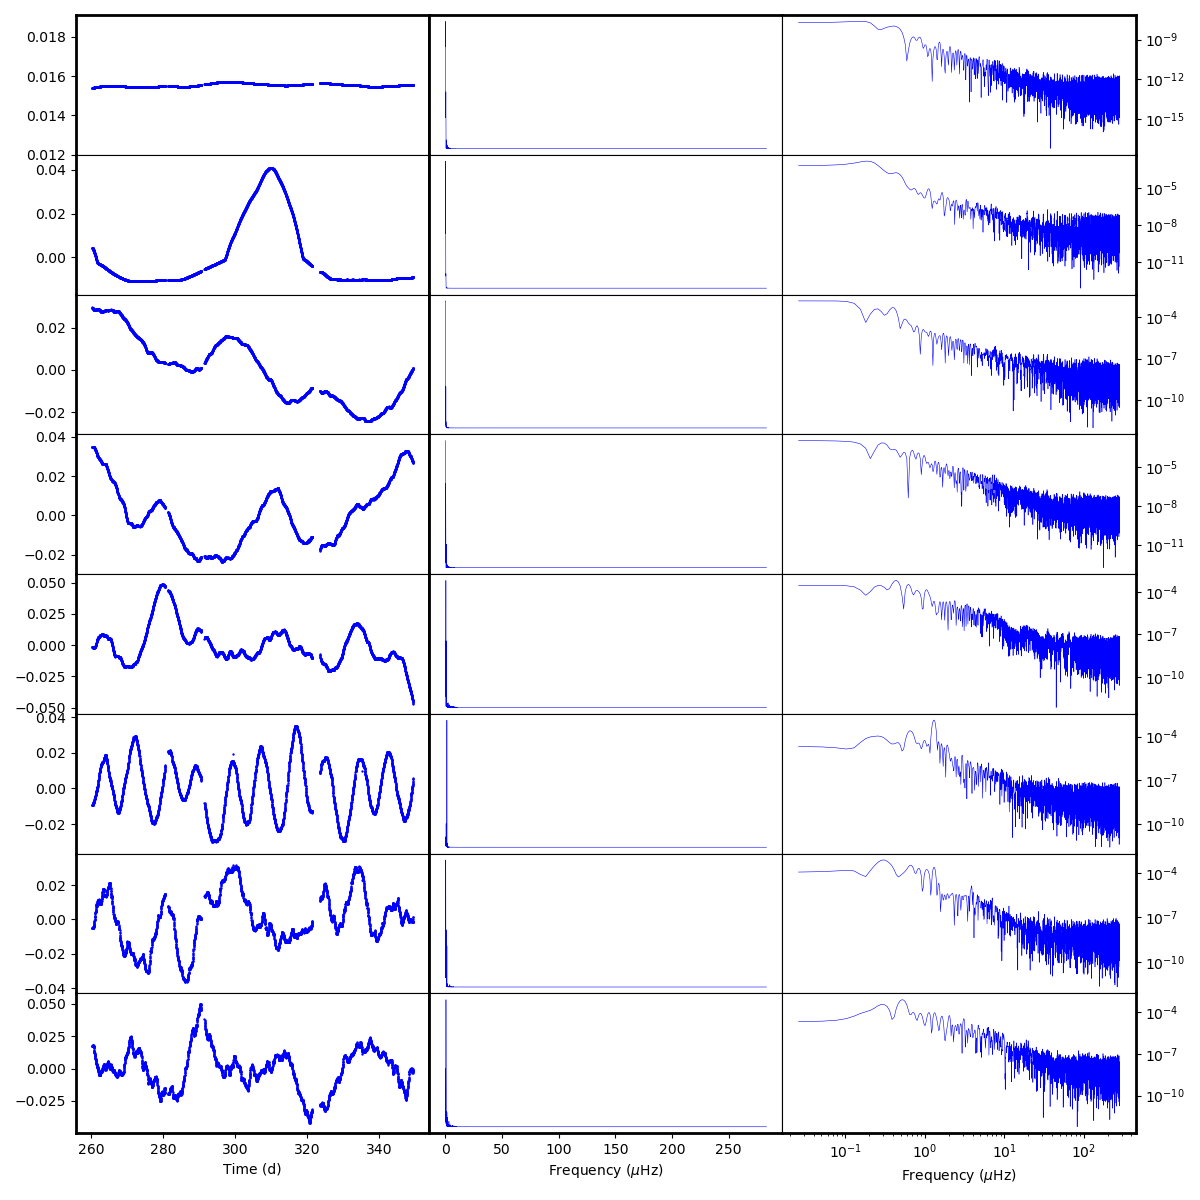
\includegraphics[width=\linewidth]{Chapter_Appended/AppB/cbv_6819_rgs_q03.png}
    \caption{Same as Figure \ref{fig:cbvs_rgsIS_6819_Q2} but for quarter 3.}
    \label{fig:cbvs_rgsIS_6819_Q03}
\end{figure}


\begin{figure}
    \centering
    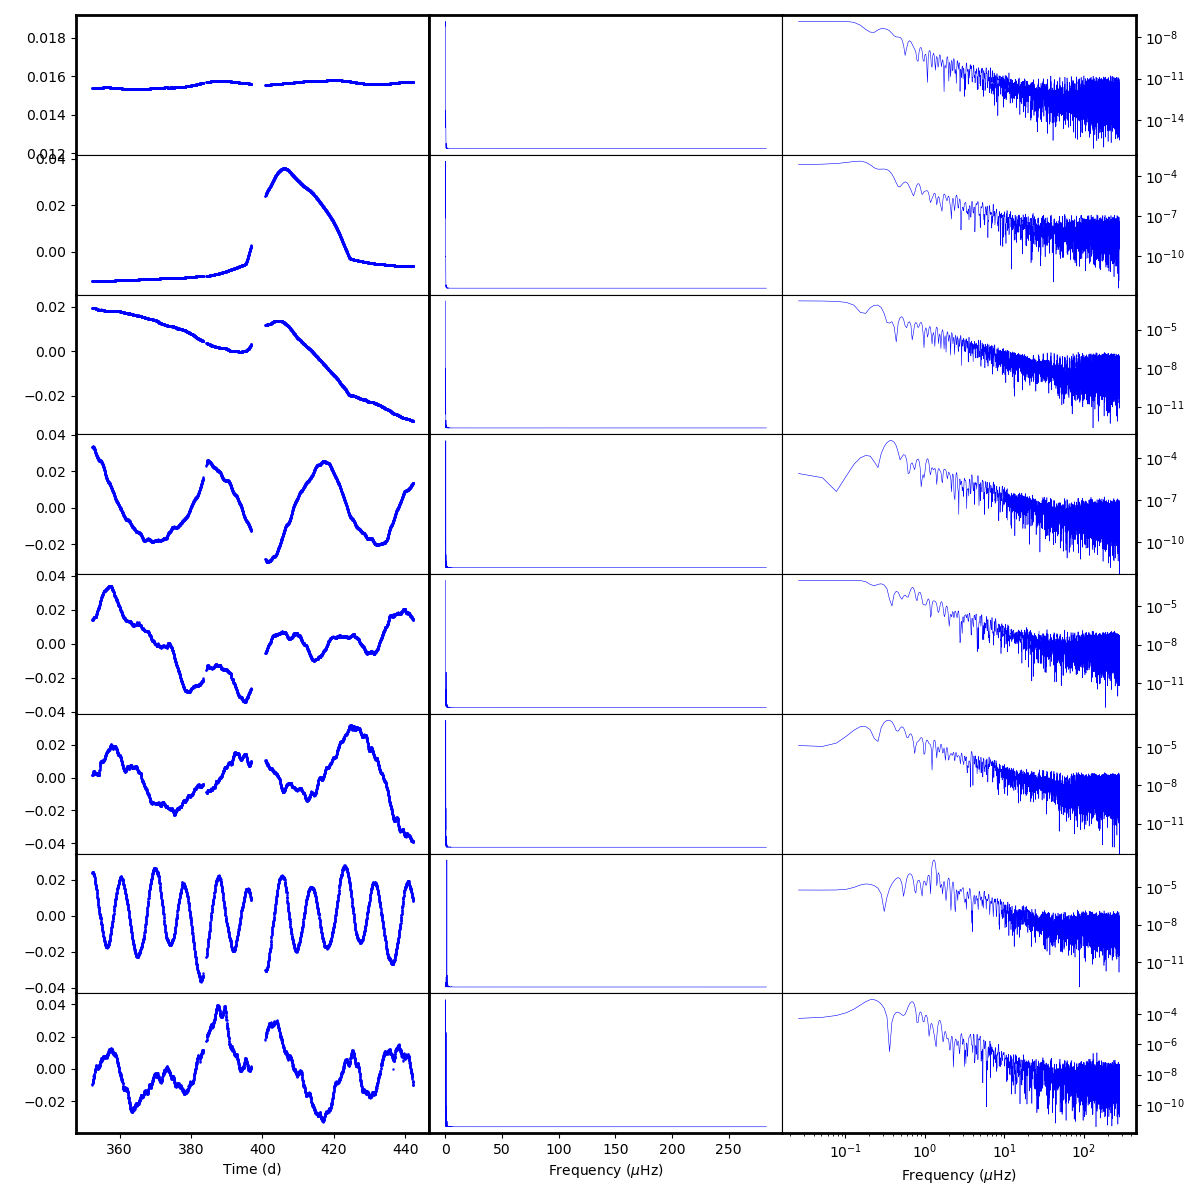
\includegraphics[width=\linewidth]{Chapter_Appended/AppB/cbv_6819_rgs_q04.png}
    \caption{Same as Figure \ref{fig:cbvs_rgsIS_6819_Q2} but for quarter 4.}
    \label{fig:cbvs_rgsIS_6819_Q04}
\end{figure}


\begin{figure}
    \centering
    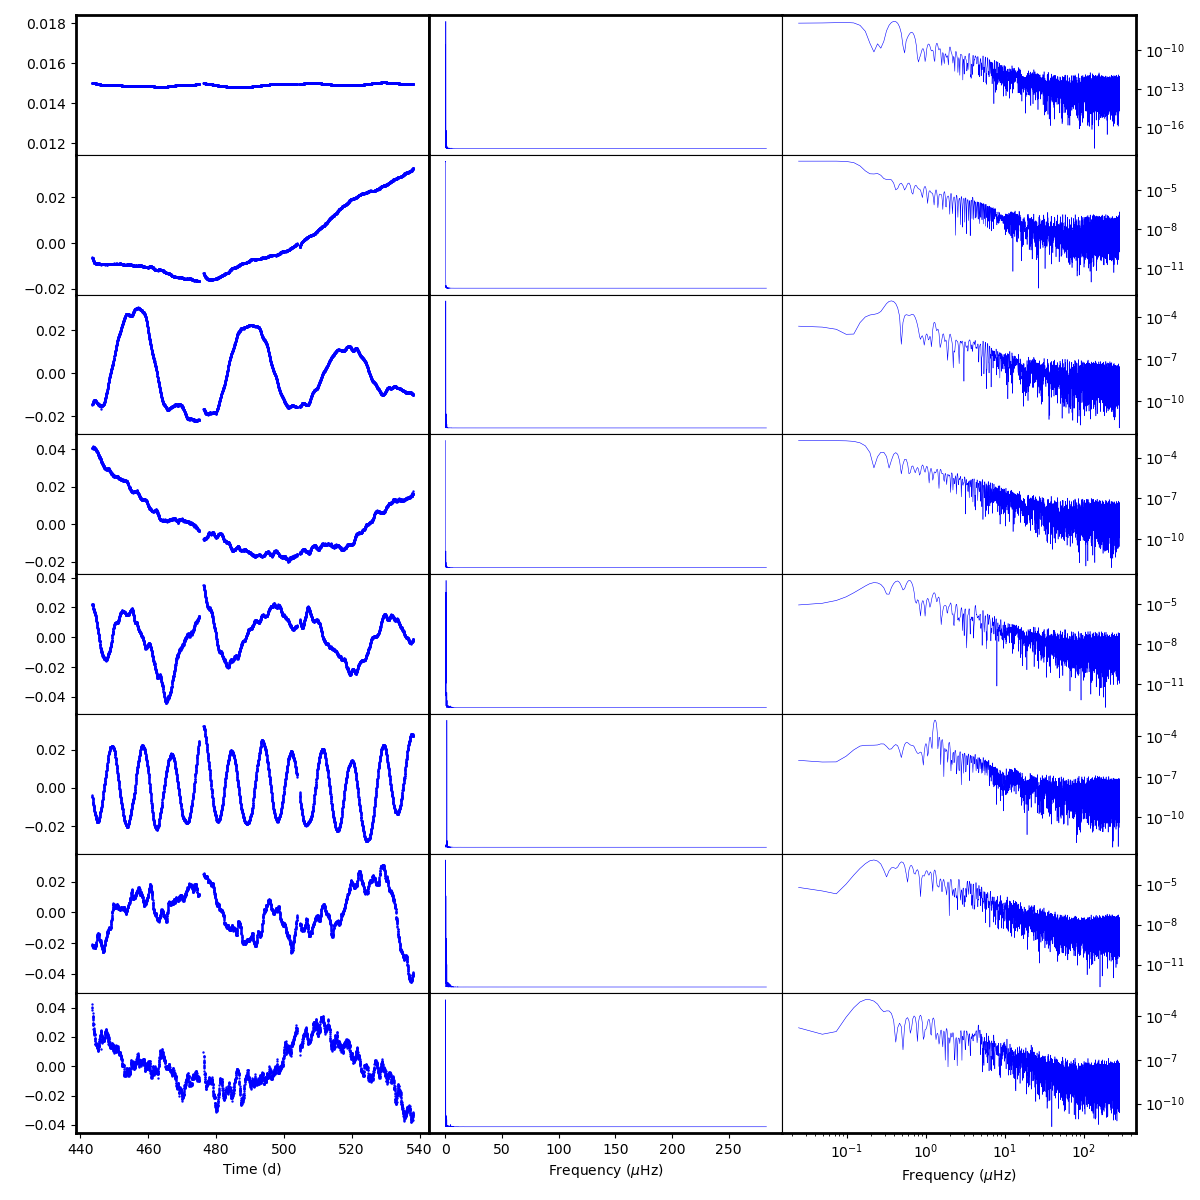
\includegraphics[width=\linewidth]{Chapter_Appended/AppB/cbv_6819_rgs_q05.png}
    \caption{Same as Figure \ref{fig:cbvs_rgsIS_6819_Q2} but for quarter 5.}
    \label{fig:cbvs_rgsIS_6819_Q05}
\end{figure}


\begin{figure}
    \centering
    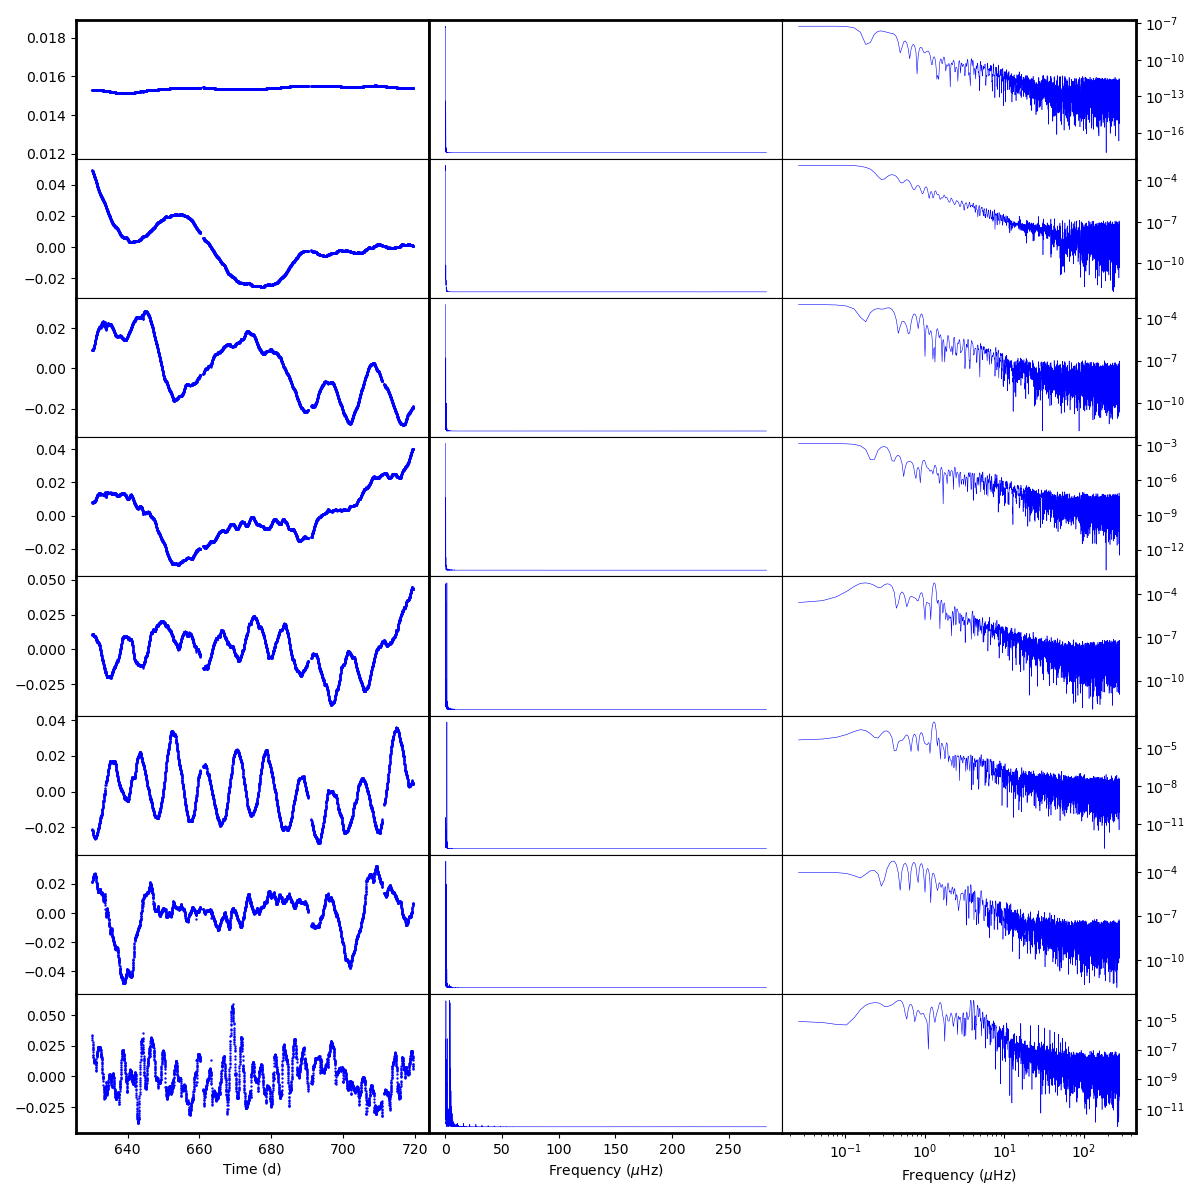
\includegraphics[width=\linewidth]{Chapter_Appended/AppB/cbv_6819_rgs_q07.png}
    \caption{Same as Figure \ref{fig:cbvs_rgsIS_6819_Q2} but for quarter 7.}
    \label{fig:cbvs_rgsIS_6819_Q07}
\end{figure}


\begin{figure}
    \centering
    \includegraphics[width=\linewidth]{Chapter_Appended/AppB/cbv_6819_rgs_q08.png}
    \caption{Same as Figure \ref{fig:cbvs_rgsIS_6819_Q2} but for quarter 8.}
    \label{fig:cbvs_rgsIS_6819_Q08}
\end{figure}


\begin{figure}
    \centering
    \includegraphics[width=\linewidth]{Chapter_Appended/AppB/cbv_6819_rgs_q09.png}
    \caption{Same as Figure \ref{fig:cbvs_rgsIS_6819_Q2} but for quarter 9.}
    \label{fig:cbvs_rgsIS_6819_Q09}
\end{figure}


\begin{figure}
    \centering
    \includegraphics[width=\linewidth]{Chapter_Appended/AppB/cbv_6819_rgs_q11.png}
    \caption{Same as Figure \ref{fig:cbvs_rgsIS_6819_Q2} but for quarter 11.}
    \label{fig:cbvs_rgsIS_6819_Q11}
\end{figure}


\begin{figure}
    \centering
    \includegraphics[width=\linewidth]{Chapter_Appended/AppB/cbv_6819_rgs_q12.png}
    \caption{Same as Figure \ref{fig:cbvs_rgsIS_6819_Q2} but for quarter 12.}
    \label{fig:cbvs_rgsIS_6819_Q12}
\end{figure}


\begin{figure}
    \centering
    \includegraphics[width=\linewidth]{Chapter_Appended/AppB/cbv_6819_rgs_q13.png}
    \caption{Same as Figure \ref{fig:cbvs_rgsIS_6819_Q2} but for quarter 13.}
    \label{fig:cbvs_rgsIS_6819_Q13}
\end{figure}


\begin{figure}
    \centering
    \includegraphics[width=\linewidth]{Chapter_Appended/AppB/cbv_6819_rgs_q15.png}
    \caption{Same as Figure \ref{fig:cbvs_rgsIS_6819_Q2} but for quarter 15.}
    \label{fig:cbvs_rgsIS_6819_Q15}
\end{figure}


\begin{figure}
    \centering
    \includegraphics[width=\linewidth]{Chapter_Appended/AppB/cbv_6819_rgs_q16.png}
    \caption{Same as Figure \ref{fig:cbvs_rgsIS_6819_Q2} but for quarter 16.}
    \label{fig:cbvs_rgsIS_6819_Q16}
\end{figure}


\begin{figure}
    \centering
    \includegraphics[width=\linewidth]{Chapter_Appended/AppB/cbv_6819_rgs_q17.png}
    \caption{Same as Figure \ref{fig:cbvs_rgsIS_6819_Q2} but for quarter 17.}
    \label{fig:cbvs_rgsIS_6819_Q17}
\end{figure}
